\documentclass{article}
% \synctex=1
% \newcommand{\fix}[1]{{\bf *** #1 ***}}
\usepackage{amsfonts, amsmath, comment, hyperref, fontawesome5}
\usepackage{mathrsfs, amssymb, tikz-cd, booktabs}
\usepackage{stmaryrd, siunitx, lmodern, multicol, adjustbox}
\usepackage{multirow, pifont, soul, enumerate}
\usepackage{latexsym, cancel, tikz, xcolor, url, color}
\usepackage{listings, amsthm}
\usepackage{imakeidx}
\usepackage[ruled,linesnumbered,boxruled,slide]{algorithm2e}
\usepackage[symbol]{footmisc}
\usepackage{textcomp}
\usepackage[T1]{fontenc}
\usepackage{marvosym}
\usepackage{harmony}
\usepackage{hieroglf}
\usepackage[noend]{algpseudocode}
\usepackage{colortbl}

\hypersetup{
    colorlinks,
    linkcolor={red!50!black},
    citecolor={blue!50!black},
    urlcolor={blue!80!black}
}

\usepackage[OT2,OT1]{fontenc}
\def\SH{\mbox{\fontencoding{OT2}\selectfont\char88}}

\newcommand\blfootnote[1]{%
    \begingroup
    \renewcommand\thefootnote{}\footnote{#1}%
    \addtocounter{footnote}{-1}%
    \endgroup
}

\linespread{1.2} 

\usepackage[all]{xy}
\usetikzlibrary{calc}
\usetikzlibrary{shapes, positioning}
\tikzset{
	arr/.style={-stealth,shorten >=4.2mm,shorten <=4.2mm,thick}, %
	dot/.style={rotate=-45,font=\LARGE}, %
	dot2/.style={rotate=45,font=\LARGE} %
}

\usepackage{amssymb}
\usepackage[many]{tcolorbox}
\newtcolorbox[auto counter,number within=section]{Question}[2][]{%
    colback=green!5,
    colframe=green!35!black,
    colbacktitle=green!35!black,
    coltitle=white,
    fonttitle=\bfseries, 
    title=Question~\thetcbcounter.\ #2,
    enhanced,
    attach boxed title to top left={yshift=-2mm, xshift=0.5cm},%
    #1% 
}

\lstset{
    basicstyle=\ttfamily, % Set the default font for listings to typewriter
    mathescape=true,      % Allows escaping to LaTeX math mode within $$
    columns=fullflexible,
    breaklines=true,      % Set automatic line breaking
    captionpos=b,         % Sets the caption-position to bottom
    xleftmargin=\parindent,
    numbers=left,         % Line numbers on left
    numberstyle=\small,   % Line numbers styling
    numbersep=5pt,
    escapeinside={(*@}{@*)} % for escaping to LaTeX inside your code
}


\makeindex

% \begin{} Basic Taken from Professor Jerry's 

%\usepackage{showlabels}
\setlength{\textheight}{8.75in}
\setlength{\textwidth}{6.5in}
\setlength{\topmargin}{0.0in}
\setlength{\headheight}{0.0in}
\setlength{\headsep}{0.0in}
\setlength{\leftmargin}{0.0in}
\setlength{\oddsidemargin}{0.0in}
\setlength{\parindent}{3pc}
\def\Z{{\mathbb{Z}}}
\def\A{{\mathbb{A}}}
\def\bbz{{\mathbb{Z}}}
\def\bbg{{\mathbb{G}}}
\def\bba{{\mathbb{A}}}
\def\End{{\rm{End}}}
\def\SL{{\rm{SL}}}
\def\s{{\rm{s}}}
\def\sm{{\rm{sm}}}
\def\lcm{{\rm{lcm}}}
\def\odd{{\rm{odd}}}
\def\even{{\rm{even}}}
\def\an{{\rm{an}}}
\def\tr{{\rm{tr}}}
\def\Tr{{\rm{Tr}}}
\def\pr{{\rm{pr}}}
\def\spr{{\rm{spr}}}
\def\min{{\rm{min}}}
\def\sk{{\rm{sk}}}
\def\ind{{\rm{ind}}}
\def\covol{{\rm{covol}}}
\def\smax{{\rm{smax}}}
\def\GL{{\rm{GL}}}
\def\rad{{\rm{rad}}}
\def\Rlk{{{\rm{Res}_{L/k}}}}
\def\tStab{{\rm{Stab}}}
\def\SO{{\rm{SO}}}
\def\PSO{{\rm{PSO}}}
\def\tSpec{{\rm{Spec}}}
\def\PGL{{\rm{PGL}}}
\def\Nm{{\rm{Nm}}}
\def\ca{{\check{a}}}
\def\cb{{\check{b}}}
\def\cI{{\check{I}}}
\def\cJ{{\check{J}}}
\def\ccc{{\check{c}}}
\def\ct{{\rm{ct}}}
\def\sf{{\rm{sf}}}
\def\sf{{\rm{sf}}}
\def\inv{{\rm{inv}}}
\def\sol{{\rm{sol}}}
\def\ram{{\rm{ram}}}
\def\Stab{{\rm{Stab}}}
\def\Sel{{\rm{Sel}}}
\def\Inv{{\rm{Inv}}}
\def\Sym{{\rm{Sym}}}
\def\Gal{{\rm{Gal}}}
\def\Cl{{\rm{Cl}}}
\def\cl{{\rm{cl}}}
\def\O{{\mathcal{O}}}
\def\M{{\mathcal{M}}}
\def\E{{\mathcal{E}}}
\newcommand{\cO}{{\mathcal{O}}}
\def\CC{{\mathcal{C}}}
\def\CS{{\mathcal{S}}}
\def\B{{\mathcal{B}}}
\def\U{{\mathcal{U}}}
\def\P{{\mathbb{P}}}
\def\I{{\mathrm{I}}}
\def\Disc{{\rm{Disc}}}
\def\disc{{\rm{disc}}}
\def\Det{{\rm{Det}}}
\def\al{{\alpha}}
\def\Aut{{\rm{Aut}}}
\def\Pic{{\rm{Pic}}}
\def\irr{{\rm{irr}}}
\def\bbp{{\mathbb{P}}}
\def\sco{{\mathscr{O}}}
\def\dim{{\rm{dim}}}
\def\red{{\rm{red}}}
\def\dcup{{\,\dot\cup}}
\def\pico{{{\rm{Pic}^1}}}
\def\tTr{{\rm{Tr}}}
\def\sep{{\rm{sep}}}
\def\Frob{{\rm{Frob}}}
\def\tSpan{{\rm{Span}}}
\def\be{{\beta}}
\def\Gr{{\rm{Gr}}}
\def\Span{{\rm{Span}}}
\def\r{{\rm{r}}}
\def\Res{{\rm{Res}}}
\def\Vol{{\rm{Vol}}}
\def\R{{\mathbb{R}}}
\def\F{{\mathbb{F}}}
\def\scj{{\mathcal{J}}}
\def\T{{\mathcal{T}}}
%{\def\L{{\mathcal{L}}
\renewcommand{\L}{\mathcal{L}}
\newcommand{\cL}{\mathcal{L}}
\def\tEnd{{\rm{End}}}
\def\Ind{{\rm{Ind}}}
\def\tdiv{{\rm{div}}}
\def\rV{{\mathrm{V}}}
\def\bbr{{\mathbb{R}}}
\def\bbq{{\mathbb{Q}}}
\def\N{{\mathbb{N}}}
\def\FF{{\mathcal{F}}}
\def\FFF{{\mathfrak{F}}}

\def\mfm{{\mathfrak{m}}}
\def\mfp{{\mathfrak{p}}}
\def\mfq{{\mathfrak{q}}}

\def\GG{{\mathcal{G}}}
\def\RR{{\mathcal{R}}}
\def\Q{{\mathbb{Q}}}
\def\bbq{{\mathbb{Q}}}
\def\sco{{\mathcal{O}}}
\def\H{{\mathcal{H}}}
\def\J{{\mathcal{J}}}
\def\U{{\mathcal{U}}}
\def\V{{\mathbb{V}}}
\def\D{{\mathcal{D}}}
\def\Z{{\mathbb{Z}}}
\def\G{{\mathbb{G}}}
\def\P{{\mathbb{P}}}
\def\F{{\mathbb{F}}}
\def\Q{{\mathbb{Q}}}
\def\C{{\mathbb{C}}}
\def\H{{\mathcal{H}}}
\def\W{{\mathcal{W}}}
\def\S{{\mathbb{S}}}
\def\Sp{{\rm{Sp}}}
\def\s{{\mathcal{S}}}
%\def\mathcalJ{{C}}
\def\cc{{\check{c}}}
\def\ci{{\check{I}}}
\def\cj{{\check{J}}}

\def\Hom{{\rm Hom}}

\def\bh{{\bf h}}
\def\ba{{\bf a}}
\def\bb{{\bf b}}
\def\id{{\rm id}}
\def\im{{\rm im}}
\def\nullity{{\rm nullity}}
\def\rank{{\rm rank}}
\def\sgn{{\rm sgn}}
\def\deg{{\rm deg}}
\def\PSO{{\rm PSO}}
\def\max{{\rm max}}
\def\ab{{\rm ab}}
\def\unr{{\rm unr}}
\def\nmax{{\rm nmax}}
\def\LT{{\rm LT}}
\def\proj{{\rm{proj}}}
\def\perp{{\rm{perp}}}
\def\refl{{\rm{refl}}}
\def\Null{{\rm{Null}}}
\def\Col{{\rm{Col}}}
\def\Row{{\rm{Row}}}
\DeclareMathOperator{\nic}{\operatorname{n-ic}}
\def\univ{{\rm univ}}
\def\Span{{\rm span}}
\def\TT{\mathbb{T}}
\def\ob{\rm{Ob\;}}
\def\hom{\rm{Hom}}
\def\div{{\rm div}}
\def\grad{{\rm grad \;}}
\def\Hess{{\rm Hess \;}}
\def\rec{{\rm{rec}}}
\def\conv{{\rm{conv}}}
\def\cone{{\rm{cone}}}
\def\size{{\rm{size}}}
\def\dist{{\rm{dist}}}
\def\diam{{\rm{diam}}}

% \end{}

\def\v{{\vspace{5pt}}}

\newcommand{\bskip}{\ldots\ldots\ldots \bigskip}
\newcommand{\micropar}[1]{\marginpar{\raggedright \fontsize{4pt}{1pt}\selectfont\textcolor{gray}{#1}}}
\newcommand{\mpar}[1]{\marginpar{\raggedright \tiny\textcolor{gray}{#1}}}
\newcommand{\add}[1]{{\color{blue} #1}}
\newcommand{\alert}[1]{{\color{red} #1}}

\renewcommand{\lg}[2]{\Big(\frac{#1}{#2}\Big)}
\newcommand{\leg}[2]{\Big(\frac{#1}{#2}\Big)}

\definecolor{codegray}{gray}{0.9}
\newcommand{\code}[1]{\colorbox{codegray}{\texttt{#1}}}
    
%\begin{} ----- DEFINITION box (light yellow)

\newcounter{deff}[section]\setcounter{deff}{0}
\renewcommand{\thedeff}{\arabic{section}.\arabic{deff}}
\newenvironment{deff}[2][]{%
\refstepcounter{deff}%
\ifstrempty{#1}%
{\mdfsetup{%
    frametitle={%
    \tikz[baseline=(current bounding box.east),outer sep=0pt]
    \node[anchor=east,rectangle,fill=yellow!20]
    {\strut Definition~\thedeff};}}
}%
{\mdfsetup{%
    frametitle={%
    \tikz[baseline=(current bounding box.east),outer sep=0pt]
    \node[anchor=east,rectangle,fill=yellow!20]
    {\strut Definition~\thedeff:~#1};}}%
}%
\mdfsetup{innertopmargin=2.5pt,linecolor=yellow!20,%
    linewidth=2pt,topline=true,%
    frametitleaboveskip=\dimexpr-\ht\strutbox\relax
}
\begin{mdframed}[]\relax%
\label{#2}}{\end{mdframed}}

%\end{}

%\begin{} ----- EXAMPLE box (light green)

\newcounter{examplee}[section]\setcounter{examplee}{0}
\renewcommand{\theexamplee}{\arabic{section}.\arabic{examplee}}
\newenvironment{examplee}[2][]{%
\refstepcounter{examplee}%
\ifstrempty{#1}%
{\mdfsetup{%
    frametitle={%
    \tikz[baseline=(current bounding box.east),outer sep=0pt]
    \node[anchor=east,rectangle,fill=green!20]
    {\strut Example~\theexamplee};}}
}%
{\mdfsetup{%
    frametitle={%
    \tikz[baseline=(current bounding box.east),outer sep=0pt]
    \node[anchor=east,rectangle,fill=green!20]
    {\strut Example~\theexamplee:~#1};}}%
}%
\mdfsetup{innertopmargin=2.5pt,linecolor=green!20,%
    linewidth=2pt,topline=true,%
    frametitleaboveskip=\dimexpr-\ht\strutbox\relax
}
\begin{mdframed}[]\relax%
\label{#2}}{\end{mdframed}}

%\end{}

%\begin{} ----- THEOREM box (orange)

\newcounter{thmm}[section]\setcounter{thmm}{0}
\renewcommand{\thethmm}{\arabic{section}.\arabic{thmm}}
\newenvironment{thmm}[2][]{%
\refstepcounter{thmm}%
\ifstrempty{#1}%
{\mdfsetup{%
    frametitle={%
    \tikz[baseline=(current bounding box.east),outer sep=0pt]
    \node[anchor=east,rectangle,fill=orange!80]
    {\strut Theorem~\thethmm};}}
}%
{\mdfsetup{%
    frametitle={%
    \tikz[baseline=(current bounding box.east),outer sep=0pt]
    \node[anchor=east,rectangle,fill=orange!80]
    {\strut Theorem~\thethmm:~#1};}}%
}%
\mdfsetup{innertopmargin=2.5pt,linecolor=orange!80,%
    linewidth=2pt,topline=true,%
    frametitleaboveskip=\dimexpr-\ht\strutbox\relax
}
\begin{mdframed}[]\relax%
\label{#2}}{\end{mdframed}}

%\end{}

%\begin{} ----- LEMMA box (lavender)

\usepackage[framemethod=TikZ]{mdframed}

\newcounter{lemm}[section]\setcounter{lemm}{0}
\renewcommand{\thelemm}{\arabic{section}.\arabic{lemm}}
\newenvironment{lemm}[2][]{%
\refstepcounter{lemm}%
\ifstrempty{#1}%
{\mdfsetup{%
    frametitle={%
    \tikz[baseline=(current bounding box.east),outer sep=0pt]
    \node[anchor=east,rectangle,fill=blue!35]
    {\strut Lemma~\thelemm};}}
}%
{\mdfsetup{%
    frametitle={%
    \tikz[baseline=(current bounding box.east),outer sep=0pt]
    \node[anchor=east,rectangle,fill=blue!35]
    {\strut Lemma~\thelemm:~#1};}}%
}%
\mdfsetup{innertopmargin=2.5pt,linecolor=blue!35,%
    linewidth=2pt,topline=true,%
    frametitleaboveskip=\dimexpr-\ht\strutbox\relax
}
\begin{mdframed}[]\relax%
\label{#2}}{\end{mdframed}}

%\end{}

%\begin{} ----- PROPOSITION box (pink)

\newcounter{propp}[section]\setcounter{propp}{0}
\renewcommand{\thepropp}{\arabic{section}.\arabic{propp}}
\newenvironment{propp}[2][]{%
\refstepcounter{propp}%
\ifstrempty{#1}%
{\mdfsetup{%
    frametitle={%
    \tikz[baseline=(current bounding box.east),outer sep=0pt]
    \node[anchor=east,rectangle,fill=red!20]
    {\strut Proposition~\thepropp};}}
}%
{\mdfsetup{%
    frametitle={%
    \tikz[baseline=(current bounding box.east),outer sep=0pt]
    \node[anchor=east,rectangle,fill=red!20]
    {\strut Proposition~\thepropp:~#1};}}%
}%
\mdfsetup{innertopmargin=2.5pt,linecolor=red!20,%
    linewidth=2pt,topline=true,%
    frametitleaboveskip=\dimexpr-\ht\strutbox\relax
}
\begin{mdframed}[]\relax%
\label{#2}}{\end{mdframed}}

%\end{}

%\begin{} ----- COROLLARY box (bright green)

\usepackage[framemethod=TikZ]{mdframed}

\newcounter{corr}[section]\setcounter{corr}{0}
\renewcommand{\thecorr}{\arabic{section}.\arabic{corr}}
\newenvironment{corr}[2][]{%
\refstepcounter{corr}%
\ifstrempty{#1}%
{\mdfsetup{%
    frametitle={%
    \tikz[baseline=(current bounding box.east),outer sep=0pt]
    \node[anchor=east,rectangle,fill=green!20]
    {\strut Corollary~\thecorr};}}
}%
{\mdfsetup{%
    frametitle={%
    \tikz[baseline=(current bounding box.east),outer sep=0pt]
    \node[anchor=east,rectangle,fill=green!50]
    {\strut Corollary~\thecorr:~#1};}}%
}%
\mdfsetup{innertopmargin=2.5pt,linecolor=green!50,%
    linewidth=2pt,topline=true,%
    frametitleaboveskip=\dimexpr-\ht\strutbox\relax
}
\begin{mdframed}[]\relax%
\label{#2}}{\end{mdframed}}

%\end{}

%\begin{} ----- RESULT box (red)

\newcounter{result}[section]\setcounter{result}{0}
\renewcommand{\theresult}{\arabic{section}.\arabic{result}}
\newenvironment{result}[2][]{%
\refstepcounter{result}%
\ifstrempty{#1}%
{\mdfsetup{%
    frametitle={%
    \tikz[baseline=(current bounding box.east),outer sep=0pt]
    \node[anchor=east,rectangle,fill=red!70]
    {\strut Result~\theresult};}}
}%
{\mdfsetup{%
    frametitle={%
    \tikz[baseline=(current bounding box.east),outer sep=0pt]
    \node[anchor=east,rectangle,fill=red!70]
    {\strut Result~\theresult:~#1};}}%
}%
\mdfsetup{innertopmargin=2.5pt,linecolor=red!70,%
    linewidth=2pt,topline=true,%
    frametitleaboveskip=\dimexpr-\ht\strutbox\relax
}
\begin{mdframed}[]\relax%
\label{#2}}{\end{mdframed}}

%\end{}

%\begin{} ----- DISCOVERY box (purple)

\newcounter{discovery}[section]\setcounter{discovery}{0}
\renewcommand{\thediscovery}{\arabic{section}.\arabic{discovery}}
\newenvironment{discovery}[2][]{%
\refstepcounter{discovery}%
\ifstrempty{#1}%
{\mdfsetup{%
    frametitle={%
    \tikz[baseline=(current bounding box.east),outer sep=0pt]
    \node[anchor=east,rectangle,fill=blue!50]
    {\strut Discovery~\thediscovery};}}
}%
{\mdfsetup{%
    frametitle={%
    \tikz[baseline=(current bounding box.east),outer sep=0pt]
    \node[anchor=east,rectangle,fill=blue!50]
    {\strut Discovery~\thediscovery:~#1};}}%
}%
\mdfsetup{innertopmargin=2.5pt,linecolor=blue!65,%
    linewidth=2pt,topline=true,%
    frametitleaboveskip=\dimexpr-\ht\strutbox\relax
}
\begin{mdframed}[]\relax%
\label{#2}}{\end{mdframed}}

%\end{}

%\begin{} ----- ALGORITHM box (gray)

\newcounter{algo}[section]\setcounter{algo}{0}
\renewcommand{\thealgo}{\arabic{section}.\arabic{algo}}
\newenvironment{algo}[2][]{%
\refstepcounter{algo}%
\ifstrempty{#1}%
{\mdfsetup{%
    frametitle={%
    \tikz[baseline=(current bounding box.east),outer sep=0pt]
    \node[anchor=east,rectangle,fill=gray!45]
    {\strut Algorithm~\thealgo};}}
}%
{\mdfsetup{%
    frametitle={%
    \tikz[baseline=(current bounding box.east),outer sep=0pt]
    \node[anchor=east,rectangle,fill=gray!45]
    {\strut Algorithm~\thealgo:~#1};}}%
}%
\mdfsetup{innertopmargin=2.5pt,linecolor=gray!45,%
    linewidth=2pt,topline=true,%
    frametitleaboveskip=\dimexpr-\ht\strutbox\relax
}
\begin{mdframed}[]\relax%
\label{#2}}{\end{mdframed}}

%\end{}

%\begin{} ----- note box (orange)

\newcounter{note}[section]\setcounter{note}{0}
\renewcommand{\thenote}{\arabic{section}.\arabic{note}}
\newenvironment{note}[2][]{%
\refstepcounter{note}%
\ifstrempty{#1}%
{\mdfsetup{%
    frametitle={%
    \tikz[baseline=(current bounding box.east),outer sep=0pt]
    \node[anchor=east,rectangle,fill=white]
    {\strut Note~\thenote};}}
}%
{\mdfsetup{%
    frametitle={%
    \tikz[baseline=(current bounding box.east),outer sep=0pt]
    \node[anchor=east,rectangle,fill=red]
    {\strut Note~\thenote:~#1};}}%
}%
\mdfsetup{innertopmargin=1.5pt,linecolor=orange,%
    linewidth=2pt,topline=true,bottomline=false,rightline=false,leftline=true,
    frametitleaboveskip=\dimexpr-\ht\strutbox\relax
}
\begin{mdframed}[]\relax%
\label{#2}}{\end{mdframed}}

%\end{}

%\begin{} 

\newenvironment{solution}{\noindent {\bf Solution:}}{$\Box$ \vspace{2 ex}}

\newenvironment*{exercise}{\noindent {\textcolor{red}{\textbf{Exercise: }}}}

\newenvironment*{remarks}{\noindent {\textcolor{magenta}{\textbf{Remark: }}}}

%\end{}
\input{codestyle.tex}

\begin{document}
\title{CS 240 with Olga Veksler}
\author{Eason Li}
\date{2025 W}
\maketitle


\tableofcontents


\newpage

% *
% !
% ?
% TODO 
% FIXME: 
% // 

\begin{center}
    \add{Lecture 1 - Tuesday, January 07}
\end{center}

\section{Introduction and Asymptotic Analysis} 

\subsection{What is this course about?} 

\begin{itemize}
    \item When first learn to program, we emphasize \textcolor{blue}{correctness}; 
    \item We also concerned with \textcolor{blue}{efficiency}; \begin{itemize}
        \item Processor time; 
        \item Memory space. 
    \end{itemize}
    \item We study efficient methods of \textcolor{blue}{storing}, \textcolor{blue}{accessing}, and \textcolor{blue}{organizing} large collections of data: Some typical operations are \begin{itemize}
        \item inserting new data items; 
        \item deleting data items.
    \end{itemize}
    \item We also cover new ADTs and how to implement ADT efficiently using appropriate data structures. 
    \item We will also cover algorithms solving problems in data management, such as sorting, pattern matching, and compression. 
\end{itemize}

\subsection{Algorithm Design}

\begin{deff}[Problem \index{Problem}].
    A \textbf{problem} is a description of input and required output. 
\end{deff}

\begin{deff}[Problem Instance \index{Problem Instance}].
    A \textbf{problem instance} is one possible input for specific problem. 
\end{deff}

\begin{deff}[Algorithm \index{Algorithm}].
    An \textbf{algorithm} us a step-by-step process (can be described in finite length) for carrying out a series of computations, given an arbitrary instance $I$. 
\end{deff}

\begin{deff}[Solving \index{Solving}].
    An algorithm $A$ \textbf{solves} problem $\Pi$ if for every instance $I$ of $\Pi$, $A$ computes a valid output for instance $I$ in finite time. 
\end{deff}

\begin{deff}[Program \index{Program}].
    A \textbf{program} is an \textit{implementation} of an algorithm using a specific computer language. 
\end{deff}

\begin{discovery}[].
    In this course, we emphasize on algorithms as opposed to programs. 
\end{discovery}

\begin{thmm}[].
    In general, from problem $\Pi$ to program that solves it, we care about \begin{enumerate}
        \item \textcolor{magenta}{\textbf{Algorithm Design:}} design algorithms that solves $\Pi$; 
        \item \textcolor{magenta}{\textbf{Algorithm Analysis:}} aseess \textit{correctness} and \textit{efficiency} of algorithms; 
        \item \textcolor{magenta}{\textbf{Implementation:}} If acceptable (correct and efficient), implement algorithms, while multiple implementations are possible; 
        \item If multiple acceptable algorithms/ implementations are present, run experiments to determine a better solution. 
    \end{enumerate}
    \hl{CS240 cares about the first two steps}. 
\end{thmm}

\subsection{Pseudocode}

\begin{deff}[Pseudocode \index{Pseudocode}].
    \textbf{Pseudocode} is a method of communication algorithm to a human. 
\end{deff}

\begin{exampleee}[Example of a Pseudocode].
    
\end{exampleee}

\begin{algorithm}[H] \KwData{this text} \KwResult{how to write algorithm with \LaTeX2e } initialization\; \While{not at end of this document}{ read current\; \eIf{understand}{ go to next section\; current section becomes this one\; }{ go back to the beginning of current section\; } } \caption{How to write algorithms} \end{algorithm}

\subsection{Measuring Efficiency} 

\begin{deff}[Efficiency \index{Efficiency}].
    Efficiency refers to \begin{itemize}
        \item Running Time: aka  ``Time Complexity'', the amount of time a program takes to run; 
        \item Auxiliary Space: aka ``Space Complexity'', the amount of additional memory a program requires. 
    \end{itemize} 
\end{deff}

To determine the running time of an algorithm, there are two methods. 

\subsubsection{Method 1: Experimental Studies}

Write program implementing the algorithm and run program with inputs of \textit{varying size} and \textit{composition}. 

\begin{comm}[].
    There are shortcomings about this method: 
    \begin{itemize}
        \item implementation may be complicated/costly
        \item timings are affected by many factors
        \begin{itemize}
            \item \textcolor{red}{hardware} (processor, memory)
            \item \textcolor{red}{software environment} (OS, compiler, programming language)
            \item \textcolor{red}{human factors} (programmer)
        \end{itemize}
        \item cannot test all inputs, hard to select good \textcolor{orange}{sample inputs}
    \end{itemize}
\end{comm}

\subsubsection{Method 2: Theoretical Analysis}

\begin{thmm}[].
    Unlike experimental studies, Theoretical Analysis \begin{itemize}
        \item Does not require implementing the algorithm 
        \item Independent of hardware/software environment 
        \item Takes into account all possible input instances
    \end{itemize}
\end{thmm}

\begin{deff}[Random Access Machine (RAM) Idealized Computer Model \index{Random Access Machine (RAM) Idealized Computer Model}].
    To process theoretical analysis, we assume that we have a RAM Idealized Computer Model, which has the following features: 
    \begin{itemize}
        \item Has a set of memory cells (unbounded number), each of which is big enough to store one data item. 
        \item Any access to a memory location takes the same constant time. 
        \item Can run other primitive operations on this machine. 
        \begin{examplee}[].
            Memory access, arithmetic, etc. 
        \end{examplee}
    \end{itemize}
    \begin{comm}[].
        The assumptions may be invalid for real computers. 
    \end{comm}
\end{deff}

\begin{algo}[Theoretical Framework For Algorithm Analysis].
    \begin{itemize}
        \item Write algorithms in pseudo-code 
        \item Run algorithms on idealized computer model 
        \item Time efficiency: count \# primitive operations as a function of problem size $n$
        \item Space efficiency: count maximum \# of memory cells ever in use
    \end{itemize}
\end{algo}

\begin{comm}[].
    Pseudocode is essentially a sequence of primitive operations. 
\end{comm}

\begin{examplee}[Example of Primitive Operations].
    \begin{minipage}{0.6\textwidth}
        \begin{algorithm}[H]
            \SetAlgoLined % Use lines in the algorithm
            \KwResult{Maximum element of the array A}
            \KwIn{Array A of n integers}
            
            \textbf{Algorithm arrayMax(A, n)}\\
            \textcolor{teal}{$currentMax \leftarrow A[0]$}\;
            \For{$i \leftarrow 1$ \KwTo \textcolor{red}{\textbf{$n-1$}}}{
                \If{$\textcolor{blue}{\textbf{A[i]}} > currentMax$}{
                    $currentMax \leftarrow A[i]$\;
                }
            }
            \textcolor{orange}{\Return $currentMax$}\;
            \caption{Find the maximum element in an array}
        \end{algorithm}
    \end{minipage}\begin{minipage}{0.4\textwidth}
        \quad Examples of Primitive Operations: 
        \begin{itemize}
            \item \textcolor{red}{arithmetic: $-, +, \%, *$, mod, round} 
            \item \textcolor{teal}{assigning a value to a variable}       
            \item \textcolor{blue}{indexing into an array} 
            \item \textcolor{orange}{returning from a method}  
            \item comparisons, calling subroutine, \\ entering a loop, breaking, etc.
        \end{itemize}
    \end{minipage}
\end{examplee}

\begin{thmm}[].
    To find running time, count the number of primitive operations as a function of $n$. 
\end{thmm}

\begin{codes}[].
    For $n$ is the input size, $x^n$ is not a primitive operation since it depends on $n$, the input size, while $x^{100000000000000000000000}$ is a primitive operation. 
\end{codes}

To perform Theoretical Analysis of Running time, we want \begin{itemize}
    \item ignore multiplicative constant factors 
    \item focus on behaviour for large $n$ (i.e. ignore lower order terms) 
\end{itemize}
This means focusing on the growth rate of the function. 

\subsection{Asymptotic Analysis}

\subsubsection{Asymptotic Upper Bound}

\begin{deff}[BigO \index{BigO}].
    $f_n \in O(g_n)$ if there exist constants $c > 0$ and $n_0 \geq 0$ s.t. 
    \[ |f_n| \leq c |g_n| \qquad \text{ for all } n \geq n_0 \]
\end{deff}

\begin{examplee}[].
    \begin{center}
        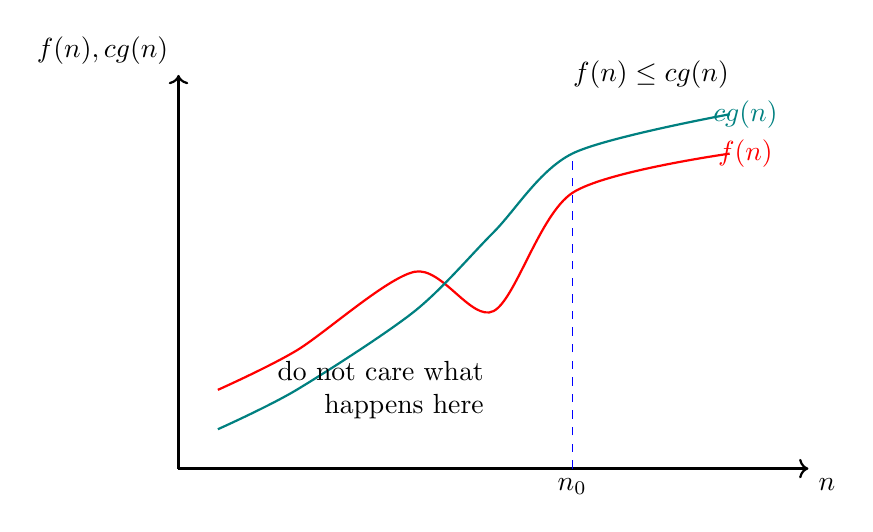
\begin{tikzpicture}
            % Draw axes
            \draw[thick,->] (0,0) -- (8,0) node[anchor=north west] {$n$};
            \draw[thick,->] (0,0) -- (0,5) node[anchor=south east] {$f(n), cg(n)$};
        
            % Draw curves
            \draw[thick, red, smooth] plot coordinates {(0.5,1) (1.5,1.5) (3,2.5) (4,2) (5,3.5) (7,4)};
            \node[red] at (7.2,4) {$f(n)$};
            \draw[thick, teal, smooth] plot coordinates {(0.5,0.5) (1.5,1) (3,2) (4,3) (5,4) (7,4.5)};
            \node[teal] at (7.2,4.5) {$cg(n)$};
        
            % Draw vertical line and labels
            \draw[dashed, blue] (5,0) -- (5,4);
            \node[anchor=north] at (5,0) {$n_0$};
            \node[anchor=east, align=right, text width=3cm] at (4, 1) {do not care what happens here};
        
            % Annotations
            \node at (6,5) {$f(n) \leq cg(n)$};
        \end{tikzpicture}
    \end{center}
\end{examplee}

\begin{result}[].
    Big-O gives asymptotic upper bound. 
\end{result}

\begin{comm}[].
    Saying ``$f_n$ is $O(g_n)$'' is equivalent to saying ``$f_n \in O(g_n)$''. 
\end{comm}

\begin{examplee}[].
    \textbf{Prove that}
    \[ 2n^2 + 3n + 11 \in O(n^2) \]
    \textbf{Need to find} $c \geq 0$ \textbf{and} $n_0 \geq 0$ \textbf{s.t.}
    \[ 2n^2 + 3n + 11 \leq cn^2 \text{ for all } n \geq n_0. \]
    Notice that \textcolor{red}{\textbf{$2n^2 + 3n + 11$}} $\leq$ \textcolor{blue}{$2n^2 + 3n^2 + 11n^2$} = \textcolor{orange}{$16n^2$} for all $n \geq 1$. Hence take $c = 16$, $n_0 = 1$. 
\end{examplee}

\begin{examplee}[].
    \textbf{Prove that}
    \[ 2n^2 \log n + 3n \in O(n^2 \log n) \]
    \textbf{Need to find} $ c > 0 $ \textbf{and} $ n_0 \geq 0 $ \textbf{s.t.}
    \[ 2n^2 \log n + 3n \leq c n^2 \log n \text{ for all } n \geq n_0. \]
    Notice that \textcolor{red}{$2n^2 \log n + 3n$} $\leq$ \textcolor{blue}{$2n^2 \log n + 3n^2 \log n$} $\leq$ \textcolor{orange}{$5n^2 \log n$} for all $n \geq 1$. Hence take $c = 5$, $n_0 = 2$. 
\end{examplee}

\begin{center}
    \add{Lecture 2 - Thursday, January 09}
\end{center}

\subsubsection{Asymptotic Lower Bound}

\begin{deff}[$\Omega$-notation \index{$\Omega$-notation}].
    We say that $f(n) \in \Omega(g(n))$ if there exists $c > 0$ and $n_0 \geq 0$ such that 
    \[ |f(n)| \geq c |g(n)| \qquad \text{ for all } n \geq n_0 \] 
\end{deff}

\begin{examplee}[].
    Show that $1/2 n^2 - 5n \in \Omega(n^2)$. We notice that 
    \[ 
        \frac{1}{2} n^2 - 5n = \frac{1}{4} n^2 + \left( \frac{1}{4} n^2 - 5n \right) \geq \frac{1}{4} n^2
    \]
    for $n > 20$. Thus we can take $c = 1/4$ and $n_0 = 20$.  
\end{examplee}

\subsubsection{Tight Asymptotic Bound}

\begin{deff}[$\Theta$-notation \index{$\Theta$-notation}].
    We say that $f(n) \in \Theta(g(n))$ if there exists $c_1, c_2 > 0$ and $n_0 \geq 0$ such that 
    \[ c_2 |g(n)| \leq |f(n)| \leq c_1 |g(n)| \qquad \text{ for all } n \geq n_0 \] 
\end{deff}

\begin{comm}[].
    $f(n) \in \Theta(g(n))$ means that $f$ and $g$ have the same growth rate. Therefore, to show that $f(n) \in \Theta(g(n))$, it is enought to show that 
    \[ f(n) \in O(g(n)) \qquad \text{ and } \qquad f(n) \in \Omega(g(n)) \]
\end{comm}

\begin{examplee}[].
    Show that $\log_b(n) \in \Theta(\log(n))$ for $b > 1$. 

    \begin{proof}
        We notice that 
        \[ \log_b(n) = \frac{\log n}{\log b} = \frac{1}{\log b} \log n \]
        Therefore, we have 
        \[ frac{1}{\log b} \log n \leq \log_b(n) \leq \frac{1}{\log b} \log n \] 
        and for $b > 1$, we have $\log b > 0$, thus we take $c_1 = c_2 = 1/ \log b$ gives us the desired result. 
    \end{proof}
\end{examplee}

\subsubsection{Common Growth Rate}

\begin{thmm}[].
    The following common growth rate are listed in increasing order: 
    \begin{center}
        \begin{tabular}{| l | r |} \hline 
            $\Theta(1)$; & Constant \\ \hline 
            $\Theta(\log n)$; & Logrithmic \\ \hline
            $\Theta(n)$; & Linear \\ \hline
            $\Theta(n \log n)$; & Linearithmic \\ \hline
            $\Theta(n \log^k n)$;  & Quasi-linear ($k$ is constant) \\ \hline
            $\Theta(n^2)$; & Quadratic \\ \hline
            $\Theta(n^3)$; & Cubic \\ \hline
            $\Theta(2^n)$. & Exponential \\ \hline
        \end{tabular}
    \end{center}
\end{thmm}

\subsubsection{Strictly Smaller Asymptotic Bound}

\begin{deff}[$o$-notation \index{$o$-notation}].
    We say $f(n) \in o(g(n))$ if for all $c > 0$, there exists $n_0$ such taht 
    \[ |f(n)| \leq c |g(n)| \qquad \text{ for all } n \geq n_0 \]
\end{deff}

\subsubsection{Strictly Larger Asymptotic Bound}

\begin{deff}[$\omega$-notation \index{$\omega$-notation}].
    We say $f(n) \in \omega(g(n))$ if for all $c > 0$, there exists $n_0$ such taht 
    \[ |f(n)| \geq c |g(n)| \qquad \text{ for all } n \geq n_0 \]
\end{deff}

\begin{thmm}[].
    We have the following: 
    \[ f(n) \in \omega(g(n)) \;\;\; \Rightarrow \;\;\; g(n) \in o(f(n)) \]
\end{thmm}

\begin{proof}
    To show that $g(n) \in o(f(n))$, we wish to show that for all $c > 0$, we know that there exists $n_0 \geq 0$ such that 
    \[ g(n) \leq c f(n) \qquad \forall \; n \geq n_0 \qquad \equiv \qquad 1/c \cdot g(n) \leq f(n) \qquad \forall \; n \geq n_0 \] 
    Since we know that $f(n) \in \omega(g(n))$, so for $c = 1/c$ in the above notation, there exists $m_0 \geq 0$ such that 
    \[ f(n) \geq 1/c \cdot g(n) \qquad \forall \; n \geq m_0 \]
    Hence we can simply take $n_0 = m_0$. 
\end{proof}

\begin{center}
    \add{Lecture 3 - Tuesday, January 14}
\end{center}

\subsubsection{Limit Theorem of Order Notation}

\begin{thmm}[Limit Theorem of Order Notation].
    Suppose for all $n \geq n_0$, we have $f(n), g(n) >0$ and $\displaystyle L = \lim_{n \to \infty} \frac{f(n)}{g(n)}$, then 
    \[ f(n) \in \begin{cases}
        o(g(n)) & \text{ if } L = 0 \\ 
        \Theta(g(n)) & \text{ if } 0 < L < \infty \\ 
        \omega(g(n)) & \text{ if } L = \infty
    \end{cases} \]
\end{thmm}

\begin{examplee}[].
    Prove that $(\log n)^a \in o(n^d)$ for any $a > 0$ and $d > 0$. 

    \begin{proof}
        Use induction to show that $\lim_n (\ln n)^k / n = 0$ for any integer $k$. Use this result to show that $\lim_n (\ln n)^a / n^d = 0$. The rest is now easy to see. 
    \end{proof}
\end{examplee}

\begin{examplee}[]. 
    Show that $f(n) := n(2 + \sin n\pi / 2) \in \Theta(n)$. 

    \begin{proof}
        We have $n \leq f(n) \leq 3n$. 
    \end{proof}
\end{examplee}

\begin{examplee}[].
    Show that $f(n) := n(1 + \sin n\pi / 2) \notin \Omega(n)$. 

    \begin{proof}
        $f$ intersects with the horizontal axis infinitely. 
    \end{proof}
\end{examplee}

\begin{result}[].
    Relationships between Order Notations: 
    \begin{itemize}
        \item $f \in \Theta(g) \iff g \in \Theta(f)$; 
        \item $f \in O(g) \iff g \in \Omega(f)$; 
        \item $f \in o(g) \iff g \in \omega(f)$; 
        \item $f \in o(g) \implies g \in O(f)$; 
        \item $f \in \omega(g) \implies g \in \Omega(f)$; 
        \item $f \in o(g) \implies g \notin \Omega(f)$; 
        \item $f \in \omega(g) \implies g \notin O(f)$; 
    \end{itemize}
\end{result} 

\subsubsection{Algebra of Order Notation}

\begin{itemize}
    \item \textbf{Identity:} $f \in \Theta(f)$;
    \item \textbf{Transitivity:} \begin{itemize}
        \item If $f \in O(g)$ and $g \in O(h)$, then $f \in O(h)$; 
        \item If $f \in \Omega(g)$ and $g \in \Omega(h)$, then $f \in \Omega(h)$; 
        \item If $f \in O(g)$ and $g \in o(h)$, then $f \in o(h)$; 
    \end{itemize}
    \item \textbf{Maximum Rules:} Suppose that $f(n), g(n) > 0$ for all $n \geq n_0$, then \begin{enumerate}
        \item $f(x) + g(x) \in O(\max \{ f(x), g(x) \})$; 
        \item $f(x) + g(x) \in \Omega(\max \{ f(x), g(x) \})$; 
    \end{enumerate}
\end{itemize}

\newpage

\subsection{Runtime Analysis}

We wish to use asymptotic notation to simplify run-time analysis. Running time of an algorithm depends on the input size $n$. 

\begin{algo}[].
    \begin{enumerate}
        \item Identify primitive operations: these require constanttime 
        \item Loop complexity expressed as sum of complexities  of each iteration 
        \item Nested loops: start with the innermost loop and proceed outwards 
        \item This gives nested summations
    \end{enumerate}
\end{algo}

\begin{examplee}[].
    \begin{algorithm}[H] 
        \KwData{an integer $n$} 
        \KwResult{how to compute complexity of an algorithm} 
        sum $\leftarrow$ $n$\;
        \For{i $\leftarrow$ 1 \emph{\KwTo} n}{ 
            \For{j $\leftarrow$ i \emph{\KwTo} n}{
                sum $\leftarrow$ sum + $(i + j)^2$
            }
        }
    \end{algorithm}
    We have \begin{align*}
        c + \sum_{i = 1}^n \sum_{j = i}^n c 
        & = c + \sum_{i = 1}^n c (n - i - 1) \\ 
        & = c + c \sum_{i = 1}^n n - c \sum_{i = 1}^n i - c \sum_{i = 1}^n 1 \\ 
        & = c \frac{n^2}{2} + c \frac{n}{2} + x
    \end{align*}
    hence the complexity of the algorithm is $\Theta(n^2)$. 
\end{examplee}

\begin{discovery}[].
    We may use $\Theta$-notation earlier, in particular, 
    \[ c + \sum_{i = 1}^n \sum_{j = i}^n c \qquad \text{ is } \qquad \Theta \left( c + \sum_{i = 1}^n \sum_{j = i}^n c \right) \]
\end{discovery}

\subsubsection{Techniques for Algorithm Analysis}

\begin{result}[Techniques for Algorithm Analysis].
    \begin{enumerate}
        \item Use $\Theta$-bounds throughout the analysis and obtain $\Theta$ bound for the complexity of the algorithm. 
        \item Prove a $O$-bound and a matching $\Omega$-bound \textit{separately}. 
    \end{enumerate}
\end{result}

\begin{examplee}[].
    \begin{algorithm}[H] 
        \KwData{an integer $n$} 
        \KwResult{how to compute complexity of an algorithm} 
        sum $\leftarrow$ $0$\;
        $i = n$\; 
        \While{$i \geq 2$}{ 
            $j = 0$\; 
            \While{$j \leq i^2$}{
                sum $\leftarrow$ sum + 1\; 
                $j = j + i$
            }
            $i = i/2$
        }
    \end{algorithm}
    \begin{itemize}
        \item Inner Loop takes $i(c)$ time; 
        \item Outer Loop takes around $\log n$ times, so 
    \end{itemize}
    \[ \sum_{i = 1}^{\log n} (1 + n / 2^{t - 1}) \in O(n) \]
\end{examplee}

\subsubsection{Worst-case/ Best-case/ Average Time Complexity}

\begin{deff}[Worst Case Running Time \index{Worst Case Running Time}].
    The \textbf{worst-case running time} of algorithm $A$ is a function $f : \Z^+ \to \R$ mapping $n$ (the input size) to the longest running time for any input instance of size $n$ 
    \[ T_{worst}(n) = \max_{I \in I_n} T(I) \] 
\end{deff}

\begin{deff}[Best Case Running Time \index{Best Case Running Time}].
    Analogous definition as above. 
\end{deff}

\begin{examplee}[].
    \begin{algorithm}[H] 
        \KwData{an array of $n$ integers} 
        \If{$n = 5$ }{
            \Return $A[0]$
        } 
        \If{$n \neq 5$ }{
            \For{$i = 1$ \emph{\KwTo} $n - 1$}{
                print$A[i]$
            }
        }
    \end{algorithm}
    The best case time complexity for the above program is $\Theta(n)$. 
\end{examplee}

\begin{center}
    \add{Lecture 4 - Thursday, January 16}
\end{center}

\begin{deff}[Average Running Time \index{Average Running Time}].
    The average-case running  time of an algorithm $A$ is function $f : \Z^+ \to \R$ mapping $n$ (input  size) to the average running time of $A$ over all instances of size $n$. 
    \[ T_{avg}(n) = \frac{1}{|I_n|} \sum_{I \in I_n} T(I) \]
\end{deff}

\begin{comm}[].
    We will assume that $I_n$ is finite. 
\end{comm}

\begin{discovery}[].
    Suppose algorithm $A$ and $B$ both solve the same problem 
    \begin{itemize}
        \item A  has worst-case runtime $O(n^3)$
        \item B  has worst-case runtime $O(n^2)$
    \end{itemize}  
    We Cannot conclude that $B$ is more efficient that $A$ because $O$-notation is only an upper bound. $A$ could have worst case runtime $O(n)$ while for $B$ the bound of $O(n^2)$ could be tight. 
\end{discovery}

\begin{algo}[].
    To compare algorithms, it is better to use $\Theta$-notation. 
\end{algo}

\newpage

\subsection{Space Analysis}

We are interested in auxiliary space, space used in addition to the space used by the input data. 

\begin{algo}[].
    To find space used by an algorithm, count total number of auxiliary memory cells  ever accessed (for reading or writing or both) by  algorithm \begin{itemize}
        \item as a function of input size $n$; 
        \item space used must always be initialized, although it may not be stated explicitly in pseudocode. 
    \end{itemize}  
\end{algo}

\subsection{Analysis of Recursive Algorithms} 

\subsubsection{Explaining Solution to a Problem}

\begin{algo}[].
    \begin{enumerate}
        \item describe the overall idea 
        \item give pseudocode or detailed description 
        \item argue correctness \begin{itemize}
            \item key ingredients, no need for a formal proof
            \item sometimes obvious enough from idea-description
        \end{itemize} 
        \item analyze runtime
    \end{enumerate}
\end{algo}

\subsubsection{Table of Recurrence Relationships}


\begin{table}[h]
    \centering
    \caption{Time Complexity Analysis for Various Recursions}
    \label{tab:recursions}
    \begin{tabular}{>{\centering\arraybackslash}m{5cm} >{\centering\arraybackslash}m{3cm} >{\arraybackslash}m{4cm}}
    \toprule
    \textbf{Recursion} & \textbf{Resolves to} & \textbf{Example} \\
    \midrule
    $T(n) \leq T(n/2) + O(1)$ & $T(n) \in O(\log n)$ & Binary search \\
    $T(n) \leq 2T(n/2) + O(n)$ & $T(n) \in O(n \log n)$ & Merge sort \\
    $T(n) \leq 2T(n/2) + O(\log n)$ & $T(n) \in O(n)$ & Heapify (*) \\
    $T(n) \leq cT(n-1) + O(1)$ for some $c < 1$ & $T(n) \in O(1)$ & Avg-case analysis (*) \\
    $T(n) \leq 2T(n/4) + O(1)$ & $T(n) \in O(\sqrt{n})$ & Range-search (*) \\
    $T(n) \leq T(\sqrt{n}) + O(\sqrt{n})$ & $T(n) \in O(\sqrt{n})$ & Interpol. search (*) \\
    $T(n) \leq T(\sqrt{n}) + O(1)$ & $T(n) \in O(\log \log n)$ & Interpol. search \\
    \bottomrule
    \end{tabular}
\end{table}

\newpage

\section{Priority Queues} 

\subsection{Abstract Data Type }

\begin{deff}[ADT \index{ADT}].
    \textbf{ADT} is a description of information and a collection of operations on that information.
\end{deff}

\begin{comm}[].
    We can have various realizations of an ADT, which specify: 
    \begin{itemize}
        \item How the information is stored (\textit{data structure}) 
        \item How the operations are performed (\textit{algorithms})
    \end{itemize}
\end{comm}

\begin{deff}[Stack \index{Stack}].
    An ADT with push and pop, LIFO. 
\end{deff}

\begin{deff}[Queue \index{Queue}].
    An ADT with enqueue and dequeue, FIFO. 
\end{deff}

\subsection{ADT Priority Queue}

Priority Queue generalizes both ADT Stack and ADT Queue. 

\begin{deff}[Priority Queue \index{Priority Queue}].
    \textbf{Priority Queue} is a collection of items (each having a priority or key) with operations \begin{itemize}
        \item insert: inserting an item tagged with a priority 
        \item delete-max: removing and returning an item of highest priority.
    \end{itemize}
\end{deff}

\subsubsection{Using a Priority Queue to sort}

\begin{algorithm}[H] 
    \KwData{an array of $n$ integers, $A[0, \ldots, n-1]$} 
    initialize $PQ$ to an empty priority queue \;
    \For{$i \leftarrow 0$ \emph{\KwTo} $n - 1$}{
        $PQ$.insert($A[i]$)
    }
    \For{$i \leftarrow n-1$ \emph{\KwTo} $0$}{
        $A[i] \leftarrow$ $PQ$.deleteMax()
    }
\end{algorithm}

\begin{comm}[].
    The runtime for the above algorithm is $O(initialization + n \cdot insert + n \cdot deleteMax)$. 
\end{comm}

\subsection{Binary Heap}

\begin{deff}[Binary Tree \index{Binary Tree}].
    A \textbf{binary tree} is either empty or contains three parts, a node and two sub binary trees. 
\end{deff}

\begin{thmm}[].
    A binary tree with $n$ nodes has height $h$: 
    \[ \log(n + 1) - 1 \leq h \leq n - 1 \]
\end{thmm}

\begin{proof}
    The upper bound is trivial, for the lower bound, we wish to saturate the lowest levels first and then calculate the possible minimal height. 
\end{proof}

\begin{deff}[Heap \index{Heap}].
    A \textbf{max-oriented binary heap} is a binary tree with the following two properties: \begin{itemize}
        \item Structural Property: \begin{itemize}
            \item All the levels of a heap are completely filled, except (possibly) for the last level. 
            \item The filled items in the last level are \textit{left-justified}. 
        \end{itemize}
        \item Heap-order Property: For any node $i$, the key of the parent of $i$ is larger than or equal to key of $i$.
    \end{itemize}
\end{deff}

\begin{codes}[].
    Heaps are ideal for implementing priority queues. 
\end{codes}

\begin{lemm}[].
    Height of a heap with $n$ nodes is $\Theta(\log n)$. 
\end{lemm}

\begin{proof}
    Since heap is a binary tree, we know that $h \in \Omega(\log n)$. STP that $h \in O(\log n)$. Since heap has full levels except level $h$, we know that 
    \[ n \geq 2^0 + 2^1 + \cdots + 2^{h-1} + 1  \]
    Solving for the inequlity we obtain that $h \leq \log n$, proving that $h \in O(\log n)$. 
\end{proof}

\begin{result}[].
    We use node and index interchangeably. \hl{Here we have some important observations:} \begin{itemize}
        \item Left child of $i$, if exists, is $2i+1$; 
        \item Right child of $i$, if exists, is $2i+2$;  
        \item Parent of $i$, if exists, is $floor[(i-1) / 2]$. 
    \end{itemize}
\end{result}

\begin{proof}
    Proof by induction. 
\end{proof}

\begin{center}
    \add{Lecture 5 - Tuesday, January 21}
\end{center}

\subsubsection{Insertion in Heaps}

\begin{algo}[].
    \begin{itemize}
        \item Place new key at the first free leaf (Heap-order property might be violated); 
        \item Perform a fix-up. 
    \end{itemize}
\end{algo}

\begin{algorithm}[H] 
    \KwData{$i$: an index corresponding to heap node} 
    initialize $PQ$ to an empty priority queue \;
    \While{$parent(i)$ exists \textbf{and} $A[parent(i)].key < A[i].key$}{
        swap $A[i]$ and $A[parent(i)]$ \\
        $i \leftarrow parent(i)$ \qquad \tcp{move to one level up}
    }
    \caption{fix-up pseudocode}
\end{algorithm}

\begin{discovery}[].
    Time: $O(tree \; heigth) = O(\log{n})$. 
\end{discovery}

\paragraph{Insert Pseudocode} \phantom{text}\\
\begin{algorithm}[H] 
    increase size \\  
    $l \leftarrow last()$ \\
    $A[l] \leftarrow x$ \\
    fix-up $(A, l)$ 
    \caption{insertion pseudocode}
\end{algorithm}

\subsubsection{deleteMax in Heaps}

\begin{algo}[].
    \begin{itemize}
        \item The root has the maximum item 
        \item Replace root by the last leaf and remove last leaf
        \item perform fix-down
    \end{itemize}
\end{algo}

\subsubsection{Fix-down}

\begin{algorithm}[H] 
    \KwData{$A$: array that stores a heap of size $n$ in locations $0,\ldots,n-1$ \\ $i$: index corresponding to a heap node} 
    \While{$i$ is not a leaf}{
        $j$ $\leftarrow$ left child of $i$ \\
        \If{$i$ has right child and $A[$right child of $i]$.key $>$ $A[$j$]$.key}{
            $j$ $\leftarrow$ right child of $i$
        } \If{$A[i].key \geq A[j].key$}{
            \textbf{break}
        } 
        swap $A[i]$ and $A[j]$ \\ 
        $i \leftarrow j$
    }
    \caption{fix-down pseudocode}
\end{algorithm}

\begin{discovery}[].
    Time: $O(tree \; heigth) = O(\log{n})$. 
\end{discovery}

\paragraph{deleteMax Pseudocode} \phantom{text}\\
\begin{algorithm}[H] 
    $l \leftarrow last()$ \\ 
    $toReturn = A[root()]$ \\ 
    $A[(root())] = A[l]$ \\ 
    decrease size \\ 
    $fix-down (A, root(), size)$
    \caption{deleteMax pseudocode}
\end{algorithm}

\subsection{PQ-Sort and Heapsort}

\begin{comm}[].
    Priority queue sort is $O (init + n \cdot insert + n \cdot deleteMax)$ time. 
\end{comm}

\begin{thmm}[].
    Heap with $n$ nodes and height $h$ has at least $n/4$ nodes at level $h-1$. 
    \label{thm2.2}
\end{thmm}

\begin{proof}
    SFAC that there are less than $n/4$ nodes at level $h-1$. It is obvious to see that the number of nodes above this level have also less than $n/4$ nodes. Moreover, for level $h$, because each node in this level must be a child of a node in level $h-1$, so there are less than $n/4 \cdot 2$ nodes at level $h$. In total, this gives us less than $n$ nodes, which is a contradiction. 
\end{proof}

\subsubsection{PQ-sort with Heaps}

\begin{algo}[].
    \begin{algorithm}[H] 
        $H \leftarrow$ empty heap \\ 
        \For{$i \leftarrow 0$ to $n-1$}{
            $H.insert(A[i])$
        } \For{$k \leftarrow n-1$ downto $0$}{
            $A[k] \leftarrow H.deleteMax()$
        }
        \caption{PQSortWithHeaps(A)}
    \end{algorithm}
\end{algo}

\begin{discovery}[].
    PQ-Sort with heap is $\Theta(n \log{n})$ and not in place. 
\end{discovery}

\subsubsection{Heapsort}

\begin{result}[].
    Heapsort: improvement to PQ-Sort with two added tricks \begin{enumerate}
        \item use the input array $A$ to store the heap! 
        \item heap can be built in linear time if know all items in advance. 
    \end{enumerate} 
\end{result}

To introduce heap sort, we first need to solve the following problem: 
\[ \texttt{build a heap from $n$ items in $A[0, \ldots, n-1]$ without using additional space. } \]
We have two choices to create heap order: namely the fix-up and fix-down method. Recall that heap with $n$ nodes and height $h$ has at least $n/4$ nodes at level $h-1$ (Theorem \ref{thm2.2}). For each of those nodes, we notice that fix-down method takes $O(1)$ time wile fix up takes $O(\log{n})$ time. Therefore, we would like to establish heap order using fix-down. One big observation is that 

\begin{comm}[].
    If both subtrees of node $v$ have correct heap-order, fix-down on $v$ will establish correct order for the whole subtree of $v$. 
\end{comm}

\paragraph{Heapify Pseudocode} \phantom{text} \\ 
\begin{algorithm}[H] 
    \KwData{$A$: an array}
    \For {$i \leftarrow parent(last())$ downto $0$}{
        $fix-down (A, i, n)$
    } 
    \caption{heapify pseudocode}
\end{algorithm}

\paragraph{Heapify Analysis}

Note that for depth $k$, there are $2^k$ nodes at most, and each of the nodes at this depth is getting moved by fix-down at most $h-k$ times. Therefore, the time is given by 
\begin{align*}
    \sum_{i = 0}^{h-1} 2^i (h - i) 
    & = 2^h \sum_{i = 0}^{h-1} \frac{h - i}{2^{h - i}} \\ 
    & = 2^h \sum_{i = 1}^{h} \frac{i}{2^i} 
\end{align*}
where we know that the latter sum is convergent. Thus 
\[ Time \leq 2^h c \leq 2^{\log{n}} c = cn \]
which proves that the time complexity of the given algorithm is $\Theta(n)$. 

Therefore, we are now able to implement the heapsort algorithm: 
\begin{algo}[].
    \begin{algorithm}[H] 
        $n \leftarrow A.size$ \\ 
        \For {$i \leftarrow parent(last())$ downto $0$}{
            $fix-down (A, i, n)$
        } 
        \While{$n > 1$}{
            swap $A[root()]$ and $A[last()]$ \\ 
            decrease $n$ \\ 
            $fix-down(A, root(), n)$
        }
        \caption{Heapsort}
    \end{algorithm}
\end{algo}

\begin{result}[ ].
    The total time is $O(n \log{n})$. 
\end{result}

\begin{Question}{Find the $k^{th}$ smallest item in an array $A$ of $n$ numbers.}
    \begin{comm}[].
        $k^{th}$ smallest = the item that would be at $A[k]$ if sorted.
    \end{comm}
\end{Question}

\begin{solution}
    We have in total three solutions so far. 
    \begin{enumerate}
        \item Make $k+1$ passes through the array, deleting the minimum number each time. 
        \null\hfill Complexity: $\theta(kn)$.

        \item Sort $A$, then return $A[k]$.
        \null\hfill Complexity: $n \log{n}$.
        
        \item Create a min-heap with $heapify(A)$. Call $delete-min(A)$ $k+1$ times.
        \null\hfill Complexity: $n + k \log{n}$.
    \end{enumerate}
\end{solution}

\newpage

\section{Sorting, Average-case and Randomization}

\begin{center}
    \add{Lecture 6 - Thursday, January 23}
\end{center}

\subsection{Analyzing average-case run-time}

\begin{examplee}[An contrived example].
    \begin{algorithm}[H] 
        \KwData{$A$: array storing $n$ distinct integers in range $\{0,1, \ldots,n-1\}$}
        \lIf{A[0]=0} { \\ 
            \lFor{$j = 1$ to n} {
                print "first is smallest"
            }} 
        \lElse{
            print "first is not smallest
        }
        \caption{smallestFirst}
    \end{algorithm}
\end{examplee}

\begin{discovery}[].
    Notice that the best case is $O(1)$ and the worst case is $\Theta(n)$.
\end{discovery}

\begin{solution}
    In general, there are $n!$ inputs in total: there are $(n-1)!$ of them having $A[0] = 0$ and the rest have the first entry non-zero. Therefore, 
    \begin{align*}
        T_{avg}(n) 
        & = \frac{1}{|I_n|} \sum_{I \in I_n} T(I) \\ 
        & = \frac{1}{n!} \left( \underbrace{cn + \cdots + cn}_{(n-1)!} + \underbrace{c + \cdots + c}_{n! - (n-1)!} \right) \\ 
        & = \frac{1}{n!} \left( cn (n-1)! + c (n! - (n-1)!) \right) \\ 
        & = c + c - \frac{c}{n} \in O(1)
    \end{align*}
\end{solution}

\begin{examplee}[Another example].
    \begin{algorithm}[H] 
        \KwData{$w$: bitstring of length $n$}
        \lIf{$n = 0$} { return true}
        \lIf{($w[n-1] = 1$)} { return false}           
        all-0-test$(w, n-1)$
        \caption{all-0-test}
    \end{algorithm}
\end{examplee}

\begin{solution}
    Best case is when the bitstring has a 1 at the end, in which case has a time complexity of $O(1)$. The worst case would be the case when the bit string has all zeros, in which case we have a time complexity of $\Theta(n)$. Let $B_n$ be the set of all bit strings of length $n$. 

    \begin{comm}[].
        Note that $|B_n| = 2 |B_{n-1}|$. 
    \end{comm}

    Hence we obtain that the average run time is 
    \[ T_{avg}(n) = \frac{1}{|B_n|} \sum_{w \in B_n} T(w) \]
    where $T(w)$ is defined as 
    \[ T(w) = \begin{cases}
        1 & \text{ if } w[n-1] = 1 \\ 
        1 + T(w[0, \ldots, n-2]) & \text{ otherwise}
    \end{cases} \]
    Therefore, we have 
    \begin{align*}
        T_{avg}(n) 
        & = \frac{1}{|B_n|} \sum_{w \in B_n} T(w) \\ 
        & = \frac{1}{|B_n|} \sum_{w \in B_n, w[n-1]=1} 1 + \frac{1}{|B_n|} \sum_{w \in B_n, w[n-1]=0} T(w) \\ 
        & = \frac{1}{|B_n|} \sum_{w \in B_n, w[n-1]=1} 1 + \frac{1}{|B_n|} \sum_{w \in B_n, w[n-1]=0} \left[ 1 +  T(w[0, \ldots, n-2]) \right] \\ 
        & = \frac{1}{2} + \frac{1}{2} + \frac{1}{|B_n|} \sum_{w \in B_n, w[n-1]=0} T(w[0, \ldots, n-2]) \\ 
        & = 1 + \frac{|B_{n-1}|}{|B_n|} \cdot \frac{1}{|B_{n-1}|} \sum_{w \in B_{n-1}} T(w) \\ 
        & = 1 + \frac{1}{2} T_{avg}(n-1)
    \end{align*}
    Hence we obtain that $T_{avg}(n)$ is $\Theta(1)$. 
\end{solution}

\subsection{Randomized Algorithms}

\begin{deff}[Randomized Algorithm \index{Randomized Algorithm}].
    A \textbf{randomized algorithm} is one which relies on random numbers for some steps
\end{deff}

\subsubsection{Expected Running Time} 

\begin{discovery}[].
    Define $T(I,R)$ to be running time of randomized algorithm for instance $I$ and $R$, sequence of random numbers algorithm choses. 
\end{discovery}

\paragraph{Expected Runtime for Instane $I$:} is expected value for $T(I, R)$: 
\[ T_{exp}(I) = \E[T(I, R)] = \sum_{R} T(I, R) \cdot Pr(R) \]

\paragraph{Worst-case Expected Runtime:} is given by 
\[ T_{exp}(n) = \max_{I \in I_n} T_{exp}(I) \]

\begin{examplee}[].
    \begin{algorithm}[H] 
        \KwData{$A$: array storing $n$ numebrs}
        $sum \leftarrow 0$ \\ 
        \lIf{$random(3) = 0$} {
            return sum} 
        \lElse{ \\
            \> \lFor{$i \leftarrow 0$ to $n - 1$} { \\
                \> \> $sum \leftarrow sum + A[i]$ 
            }
            return sum
        }
        \caption{simple}
    \end{algorithm}
\end{examplee}

\begin{solution}
    Notice that the algorithm needs only one random number, and 
    \[ Pr(0) = Pr(1) = Pr(2) = \frac{1}{3} \]
    Hence we have \begin{align*}
        T_{exp}(I) 
        & = T(I, 0) \cdot Pr(0) + T(I, 1) \cdot Pr(1) + T(I, 2) \cdot Pr(2) \\ 
        & = c \cdot \frac{1}{3} + c \cdot n \cdot \frac{1}{3} + c \cdot n \cdot \frac{1}{3} \in \Theta(n)
    \end{align*}
    as desired. 
\end{solution}

\begin{examplee}[].
    \begin{algorithm}[H] 
        \KwData{$A$: array storing $n$ numebrs}
        $sum \leftarrow 0$ \\ 
        $r1 \leftarrow random(n)$, $r2 \leftarrow random(n)$ \\ 
        \For{$i \leftarrow 1$ to $r1$}{
            \For{$j \leftarrow 1$ to $r2$}{
                $sum \leftarrow sum + A[j]A[i]$
            }
        }
        \caption{simple2}
    \end{algorithm}
\end{examplee}

\begin{solution}
    We have \begin{align*}
        T_{exp}(I)
        & = \sum_{\langle r_1, r_2 \rangle} T(I, \langle r_1, r_2 \rangle) \cdot \left( \frac{1}{n} \right)^2 \\ 
        & = \left( \frac{1}{n} \right)^2 \sum_{r1 \in \{0, \ldots, n-1\}} c \cdot r_1 \sum_{r_2 \in \{0, \ldots, n-1\}} r_2 \\ 
        & = \left( \frac{1}{n} \right)^2 \sum_{r_1 \in \{0, \ldots, n-1\}} c \cdot r_1 \frac{n (n-1)}{2} \\ 
        & = \left( \frac{1}{n} \right)^2 c \frac{n (n-1)}{2} \frac{n (n-1)}{2}
    \end{align*}
    All instances have the same running time, so $T_{exp}(n) \in \Theta(n^2)$. 
\end{solution}

\begin{Question}{Why do we use Randomized Algorithms}
    \begin{itemize}
        \item improved running time; 
        \item improve solution. 
    \end{itemize}
\end{Question}

\begin{result}[].
    Randomization can shift dependence from what we cannot control (user) to what we can control (random number generation). 
\end{result}

\paragraph{The following algorithm essentially does the same thing as the algorithm ``all-0-test'', but with randomization:} 
\begin{algo}[].
    \begin{algorithm}[H] 
        \tcp{test if all entries of bitstring $w[0,\ldots,n-1]$ are 0}
        \If{$(n = 0)$}{\Return{true}}
        \If{$(random(2) = 0)$}{
            $w[n-1] = 1 - w[n-1]$
        }   
        \If{$(w[n-1] = 1)$}{\Return{false}}
        randomized-all-0-test(w,n-1)
        \caption{randomized-all-0-test}
    \end{algorithm}
\end{algo}

\begin{solution}
    Let $T(w, R)$ be the number of bit-comparisons on input $w$ if the random outcomes are $R$. We have 
    \[ R = \langle x, R' \rangle \] 
    where $x$ is the first random number and $R'$ are the other random numbers (if any) for the recursions. 
    \begin{comm}[].
        By random number independence, $Pr(R) = Pr(x) \cdot Pr(R')$. 
    \end{comm} 
    Hence we have \begin{align*}
        T_{exp}(w) 
        & = \sum_{R} Pr(R) \cdot T(w, R) \\ 
        & = \sum_{\langle x, R' \rangle} Pr(R') Pr(x) \cdot T(w, \langle x, R' \rangle) \\ 
        & = \frac{1}{2} \sum_{\langle x, R' \rangle} Pr(R') \cdot T(w, \langle x, R' \rangle) \\ 
        & = \frac{1}{2} \sum_{R'} Pr(R') \cdot T(w, \langle x=w[n-1], R' \rangle) + \frac{1}{2} \sum_{R'} Pr(R') \cdot T(w, \langle x \neq w [n-1], R' \rangle) \\ 
        & = \frac{1}{2} \sum_{R'} 1 + \frac{1}{2} \sum_{R'} Pr(R') \cdot (1 + T(w[0..n-2], R')) \\ 
        & = \frac{1}{2} + \frac{1}{2} \sum_{R'} Pr(R') + \frac{1}{2} \sum_{R'} Pr(R') \cdot T(w[0..n-2], R') \\ 
        & = \frac{1}{2} + \frac{1}{2} + \frac{1}{2} \sum_{R'} Pr(R') \cdot T(w[0..n-2], R') \\ 
        & = 1 + \frac{1}{2} T_{exp} (\text{some instance of size } n-1) \\ 
        & \leq 1 + \max_{v \in B_{n-1}} T_{exp} (v) \\ 
        & = 1 + \frac{1}{2} T_{exp}(n-1) 
    \end{align*}
    Sicne we know that the inequality is true for all $w$, hence 
    \[ T_{exp}(n) = \max_{w \in B_n} T_{exp}(w) \leq 1 + \frac{1}{2} T_{exp}(n-1) \]
    which is a recurrence relation resolves to $\Theta(1)$. 
\end{solution} 

\begin{discovery}[].
    Average case runtime and expected runtime are different concepts!
\end{discovery} 

\newpage

\begin{result}[].
    \begin{center}
        \begin{tabular}{c | c}
            \textbf{average vase} & \textbf{expected} \\ \hline
            $\displaystyle T^{avg}(n) = \frac{\sum_{I \in I_n} T(I)}{|I_n|}$ & $\displaystyle T^{exp}(I) = \sum_{R} T(I, R) \cdot Pr(R)$ \\ 
            sum is over instances & sum is over random outcomes \\ 
            & \hl{applied only to a randomized algorithm}
        \end{tabular}
    \end{center}
\end{result}

\begin{center}
    \add{Lecture 7 - Tuesday, January 28}
\end{center}

\subsection{QuickSelect}

Given array $A$ of $n$ numbers, and $0 \leq k < n$, find the element that would be at position $k$ if $A$ was sorted. 

\begin{deff}[Rank \index{Rank}].
    $k$ is also known as \textbf{rank}. 
\end{deff}

\begin{comm}[].
    A special case is when $\displaystyle k = \lfloor \frac{n}{2} \rfloor$, which is known as \texttt{MedianFinding}. 
\end{comm}

\begin{thmm}[].
    Selection can be done with heaps in $\Theta (b + k \log{n})$ time. 
\end{thmm}

\begin{Question}{Can we do selection in linear time?}
    Yes, with quick-select (average case analysis). 
\end{Question}

\subsubsection{Two Crucial Subroutines for Quick-Select}

\begin{codes}[].
    \begin{itemize}
        \item \code{choose-pivot(A)}: return an index $p$ in $A$, $v = A[p]$ is called \textbf{pivot value}; 
        \item \code{partition(A, p)}: uses $v = A[p]$ to rearranges $A$ so that \begin{align*}
            A[m] & \leq v \quad \forall m \in \{0, \ldots, i-1\}, \\ 
            A[i] & = v, \\ 
            A[n] & \geq v \quad \forall n \in \{i+1, \ldots, n-1\} \\ 
        \end{align*}
    \end{itemize}
\end{codes}

\subsubsection{Partition}

\begin{algorithm}[H]
    \SetAlgoLined % Use lines in the algorithm
    \KwIn{Array A of size n, p is an integer such that $0 \leq p < n$}
    
    \textbf{partitian(A, p)}\\
    create empty lists small, equal and large \\
    $v \leftarrow A[p]$ \\
    \For{each element $x$ in $A$}{
        if $x < v$ then $small.append(x)$ \\
        else if $x > v$ then $large.append(x)$ \\
        else $equal.append(x)$ 
    } 
    $i \leftarrow small.size$ \\ 
    $j \leftarrow equal.size$ \\ 
    overwrite $A[0,\ldots, i-1]$ by elements in small \\ 
    overwrite $A[i,\ldots, i+j-1]$  by elements in equal \\ 
    overwrite $A[i+j,\ldots,n-1]$ by elements in large \\ 
    \Return $i$\;
    \caption{partition}
\end{algorithm}

\begin{comm}[].
    The above is an easy linear-time implementation using extra (auxiliary) $\Theta(n)$ space, we wish to have $\Theta(1)$ space. 
\end{comm}

\begin{algorithm}[H]
    \DontPrintSemicolon  % Turn off semicolon usage
    \caption{Partition the array using a pivot}
    \KwIn{Array $A$ of size $n$, pivot index $p$ such that $0 \leq p < n$}
    
    swap($A[n-1], A[p]$)\tcp*[r]{Put pivot at the end}
    $i \gets -1$, $j \gets n - 1$, $v \gets A[n-1]$\;
    
    \textbf{Loop:}
    \>\>\>\> do $i \leftarrow i+1$  while $A[i] < v$ \; 
    \>\>\>\> do $j \leftarrow j-1$  while $j \geq i$ and $A[j] > v$ \; 
    \>\>\>\> if $i \geq j$ then break \; 
    \>\>\>\> else $swap(A[i] , A[j])$ \;
    \textbf{End loop}
    
    swap($A[n-1], A[i]$)\tcp*[r]{Put pivot in the correct position}
    \Return{$i$}\;
\end{algorithm}

\begin{algo}[].
    The partition algorithm below is an efficient in-place partition whose running time is $\Theta(n)$. 
\end{algo}

Now we may introduce the quickselect algorithm: 

\begin{codes}[QuickSelect].
    \begin{algorithm}[H]
        \SetAlgoLined % Use lines in the algorithm
        \KwIn{Array A of size n, k is an integer such that $0 \leq k < n$}
        
        \textbf{quickSelect(A, k)}\\
        $p \leftarrow choose-pivot(A)$ \\ 
        $i \leftarrow partition(A, p)$ \\ 
        if $i = k$ then \Return $A[i]$\;  
        else if $i > k$ then \Return $quickSelect(A[0, \ldots, i-1], k)$
        else if $i < k$ then \Return $quickSelect(A[i+1, \ldots, n-1], k-(i+1))$
        \caption{QuickSelect}
    \end{algorithm}
\end{codes}

\begin{result}[].
    Let $T(n,k$ be \# of comparisons in array of size $n$ with parameter $k$. \begin{itemize}
        \item \textit{Best Case}: First chosen pivot could have pivot index $k$, hence no recursive call, total cost is $\Theta(n)$
        \item \textit{Worst Case}: Pivot value is always the largest and $k = 0$, in which case we have a recursive relation
        \[ T(n, 0) = \begin{cases}
            T(n - 1, 0) & n > 1 \\ 
            1 & n = 1
        \end{cases} \]
        which resolves to $\Theta(n^2)$. 
    \end{itemize}
\end{result}

\subsubsection{Average Case Analysis for QuickSelect}

the expected time of randomized QuickSelect is the same as average case runtime of nonrandomized QuickSelect. 

\begin{thmm}[].
    We can show (complicated) that the average case runtime for QuickSelect is $\Theta(n)$. 
\end{thmm}

\begin{discovery}[].
    Instead, we will randomize QuickSelect, so that the expected time of randomized QuickSelect is the same as average case runtime of nonrandomized QuickSelect. 
\end{discovery}

\paragraph{Randomization} 

\subparagraph{Idea 1: Shuffle the input then run QuickSelect} 
\phantom{test} \\
\begin{algorithm}[H]
    \SetAlgoLined % Use lines in the algorithm
    \KwIn{Array A of size n}
    
    \textbf{quickSelectShuffled(A, k)}\\
    \For{$i \leftarrow 1$ to $n-1$}{
        $swap(A[i], A[random(1 + i)])$
    }
    \caption{quickSelectShuffled}
\end{algorithm}

\begin{comm}[].
    Can show that every permutation of $A$ is equally likely after shuffle. 
\end{comm}

\subparagraph{Idea 2: Change pivot selection}
\phantom{text} \\ 
\begin{algorithm}[H]
    \SetAlgoLined % Use lines in the algorithm
    \KwIn{Array A of size n, k: integer such that $0 \leq k < n$}
    
    \textbf{randomizedQuickSelect(A, k)}\\
    $p \leftarrow random(A.size)$ \\ 
    $i \leftarrow partition(A, p)$ \\ 
    if $i = k$ then \Return $A[i]$ \\ 
    else if $i > k$ then \\ 
    \>\> \Return $randomizedQuickSelect(A[0, \ldots, i-1], k)$ \\ 
    else if $i < k$ then \\ 
    \>\> \Return $randomizedQuickSelect(A[i+1, \ldots, n-1], k-(i+1))$ 
    \caption{randomizedQuickSelect}
\end{algorithm}

Now we perform the runtime analysis. Let $T(A, k, R)$ be the number of key-comparisons on array $A$ of size $n$, selecting $k$th element, using random numbers $R$. Hence $R$ is a sequence of randomly generated pivot indexes, 
\[ R = \langle first, rest \rangle = \langle i, R' \rangle \]
Structure of array $A$ after partition is in the form of 
\begin{center}
    \begin{tabular}{|c|c|c|}
        \hline
        B & v & C \\ \hline
    \end{tabular}
\end{center}
where $B$ has a size of $i$ and $C$ has a size of $n-i-1$. Recurse in array $B$ or $C$ or algorithms stops: 
\[ T(A, k, \langle i, R' \rangle) = \begin{cases}
    T(B, k, R') & i > k \\ 
    T(C, k-i-1, R') & I < k \\ 
    0 & otherwise
\end{cases} \]
Notice that the runtime of \code{randomizedQuickSelect(A, k)} also depends on $k$: 
\[ T^{exp}(n) = \max_{A \in I_n} \max_{k \in \{0, \ldots, n-1\}} \sum_{R} T(A, k, R) Pr(R) \]
Hence 
\begin{align*}
    \sum_{R} T(A, k, R) Pr(R)
    & = \sum_{\langle i, R' \rangle} T(A, k, \langle i, R' \rangle) Pr(\langle i, R' \rangle) \\ 
    &= \sum_{R = \langle i,R' \rangle} T(A, k, \langle i, R' \rangle) \Pr(i) \Pr(R') \\
    &= \frac{1}{n} \sum_{i = 0}^{k-1} \sum_{R'} T(A, k, \langle i, R' \rangle)) \Pr(R') + \frac{1}{n} \sum_{i=k+1}^{n-1} \sum_{R'} T(A, k, \langle i, R' \rangle) \Pr(R') \\
    &= \frac{1}{n} \sum_{i=0}^{k-1} \sum_{R'} [n + T(C, k-i-1, R')] \Pr(R') + 1 + \frac{1}{n} \sum_{i=k+1}^{n-1} \sum_{R'} [n + T(B, k, R')] \Pr(R') \\
    &\leq n + \frac{1}{n} \sum_{i=0}^{k-1} \max_{D \in I_{n-i-1}, w \in \{0, \ldots, k-1\}} \sum_{R'} T(D, w, R') \Pr(R') \\
    &\quad + \frac{1}{n} \sum_{i=k+1}^{n-1} \max_{D \in I_i, w \in \{k+1, \ldots, n-1\}} \sum_{R'} T(D, w, R') \Pr(R') \\
    &= n + \frac{1}{n} \sum_{i=0}^{k-1} T^{\text{exp}}(n - i - 1) + \frac{1}{n} \sum_{i=k+1}^{n-1} T^{\text{exp}}(i)
\end{align*}
Since above bound works for any $A$ and $k$, it will work for the worst $A$ and $k$. 
\begin{tcolorbox}[ams align*,colback=yellow!10!white,colframe=orange]
    T^{\text{exp}}(n) 
    & = \max_{A \in I_n} \max_{k \in \{0, \ldots, n-1\}} \sum_{R} T(A, k, R) \Pr(R) \\
    & \leq n + \frac{1}{n} \sum_{i=0}^{n-1} \max \{ T^{\text{exp}}(i), T^{\text{exp}}(n - i - 1) \} 
\end{tcolorbox}

\begin{thmm}[].
    For the above $T(n)$, we have 
    \[ T(n) \in O(n) \]
\end{thmm}

\begin{proof}
    We will prove $T(n) \leq 4 n$ by induction on $n$. 
    \begin{itemize}
        \item \texttt{Base case:} when $n = 1$, we have $T(n) = 1 \leq 4$. 
        \item \texttt{Induction Hypethesis:} We have \begin{align*}
            T(n)
            & \leq n + \frac{1}{n} \sum_{i=0}^{n-1} \max\{T(i), T(n-i-1)\} \\
            & \leq n + \frac{1}{n} \sum_{i=0}^{n-1} \max\{4i, 4(n-i-1)\} \\
            & \leq n + \frac{4}{n} \sum_{i=0}^{n-1} \max\{i, n-i-1\}
        \end{align*}
        Continue on next page: \begin{align*}
            \sum_{i=0}^{n-1} \max(i, n-i-1) 
            & = \left( \sum_{i=0}^{\frac{n}{2}-1} \max(i, n-i-1) \right) + \left( \sum_{i=\frac{n}{2}}^{n-1} \max(i, n-i-1) \right) \\
            & = \left( \max(0, n-1) + \max(1, n-2) + \max(2, n-3) + \ldots + \max\left(\frac{n}{2}-1, n - \left(\frac{n}{2}-1\right) - 1\right) \right) \\ 
            & + \left( \max\left(\frac{n}{2}, n - \frac{n}{2} - 1\right) + \ldots + \max(n-1, 0) \right) \\ 
            & = \left( (n-1) + (n-2) + \ldots + \frac{n}{2} \right) + \left( \frac{n}{2} + (\frac{n}{2}+1) + \ldots + (n-1) \right) \\
            & = \left(\frac{3n}{2} - 1\right) \frac{n}{4} + \left(\frac{3n}{2} - 1\right) \frac{n}{4} \\ 
            & \leq \frac{3}{4} n^2
        \end{align*}
    \end{itemize}
    as desired. 
\end{proof}

\subsection{QuickSort} 

\begin{algorithm}[H]
    \DontPrintSemicolon  % Suppresses the end-of-line semicolon
    \caption{QuickSort Algorithm}
    \KwIn{Array $A$ of size $n$}
    \KwOut{Sorted Array $A$}
    
    \SetKwFunction{FQuickSort}{QuickSort}
    \SetKwFunction{FPartition}{partition}
    \SetKwFunction{FChoosePivot}{choose-pivot}
    
    \SetKwProg{Fn}{Function}{:}{}
    \Fn{\FQuickSort{$A$}}{
        \If{$n \leq 1$}{
            \Return\;
        }
        $p \gets \FChoosePivot{(A)}$\;
        $i \gets \FPartition{(A, p)}$\;
        \FQuickSort{$A[0, \ldots, i-1]$}\;
        \FQuickSort{$A[i+1, \ldots, n-1]$}\;
    }
\end{algorithm}

\begin{discovery}[].
    \begin{itemize}
        \item \textit{Worst case}: $T(n) = T(n-1) + n$, which is a recurrence solved in the same way as quickSelect, $O(n^2)$; 
        \item Best case $T(n) = T(\lceil n/2 \rceil) + T(\lceil n/2 \rceil) + n$ which is solved in the same way as mergeSort, $\Theta(n \log{n})$. 
    \end{itemize}
\end{discovery}

\begin{comm}[].
    We fine the average case through randomized version of QuickSort by changing the line of initializing $p$ to 
    \[ p \leftarrow random(A.size) \]
\end{comm}

\noindent The expected running time for \code{RandomizedQuickSort}, derived similarly to \code{RandomizedQuickSelect}, is 
\[ T^{\exp}(n) \leq \frac{1}{n} \sum_{i=0}^{n-1} \left(n + T^{\exp}(i) + T^{\exp}(n - i - 1)\right) \]
hence \begin{align*}
    T^{\exp}(n)
    & \leq \frac{1}{n} \sum_{i=0}^{n-1} \left(n + T^{\exp}(i) + T^{\exp}(n - i - 1)\right) \\
    & = n + \frac{1}{n} \left(\sum_{i=0}^{n-1} T^{\exp}(i) + \sum_{i=0}^{n-1} T^{\exp}(n - i - 1)\right) \\
    & = n + \frac{2}{n} \sum_{i=0}^{n-1} T^{\exp}(i)
\end{align*}
Thus 
\begin{tcolorbox}[ams align*,colback=yellow!10!white,colframe=orange]
    T^{\text{exp}}(n) 
    \leq n + \frac{2}{n} \sum_{i=0}^{n-1} T^{\exp}(i)
\end{tcolorbox}

\begin{thmm}[].
    For the above T(n), we have 
    \[ T(n) \leq 2 n \ln{n} \qquad \text{ for all } n > 0 \]
\end{thmm}

\begin{proof}
    The proof is using induction. $T(1) = 0$ (no comparisons). Hence for $n \geq 2$
    \[ T(n) \leq n + \frac{2}{n} \sum_{i=2}^{n-1} T(i) \leq n + \frac{2}{n} \sum_{i=2}^{n-1} 2i\ln i = n + \frac{4}{n} \sum_{i=2}^{n-1} i\ln i \]
    In particular, \begin{align*}
        \sum_{i=2}^{n-1} i \ln i 
        \leq \int_2^n x \ln x \, dx 
        & = \frac{1}{2} n^2 \ln n - \frac{1}{4} n^2 \underbrace{ - 2 \ln 2 + 1}_{\leq 0} \\
        & \leq \frac{1}{2} n^2 \ln n - \frac{1}{4} n^2 
    \end{align*}
    This is tight since best-case run-time is $\Omega (n \log{n})$. 
\end{proof}

\begin{center}
    \add{Lecture 8 - Thursday, January 30}
\end{center}

\subsubsection{QuickSort with Tricks}

We have a several ways to improve our algorithm: 
\begin{itemize}
    \item We can reduce that auxiliary space to $\Theta(\log{n})$ worst-case by recurse in smaller sub-array first and replace the other recursion by a while-loop (tail call elimination); 
    \item Stop recursion when, say $n \leq 10$. At this point, array is not completely sorted, but almost sorted, hence we can run insertionSort, which sorts in just $O(n)$ time since all items are within 10 units of the required position; 
    \item In terms of implementation, instead of passing full arrays, pass only the range of indices could avoid recursion altogether by keeping an explicit stack. 
\end{itemize}

\begin{algorithm}[H]
    \SetAlgoLined
    \SetKwInOut{Input}{input}
    \SetKwInOut{Output}{output}
    
    \Input{An array $ A $ of size $ n $}
    \Output{A sorted array $ A $}
    \BlankLine
    
    \DontPrintSemicolon
    \SetKwData{Left}{left}
    \SetKwData{Right}{right}
    \SetKwData{Pivot}{pivot}
    \SetKwData{Index}{index}
    \SetKwFunction{Size}{Size}
    \SetKwFunction{ChoosePivot}{choose-pivot}
    \SetKwFunction{Partition}{partition}
    \SetKwFunction{Push}{push}
    \SetKwFunction{Pop}{pop}
    \SetKwFunction{InsertionSort}{InsertionSort}
    
    \SetKwProg{Fn}{Function}{:}{}
    \Fn{QuickSortImproves($A, n$)}{
        \textbf{initialize} a stack $ S $ of index-pairs with \{$(0, n - 1)$\}\;
        \While{$ S $ is not empty}{
            $(\Left, \Right) \leftarrow S.\Pop()$ \tcp{\textcolor{orange}{get the next subproblem}}
            \While{$\Right - \Left + 1 > 10$ \tcp{\textcolor{orange}{work on it if it's larger than 10}}}{
            \Pivot $\leftarrow$ \ChoosePivot{$A, \Left, \Right$}\;
            \Index $\leftarrow$ \Partition{$A, \Left, \Right, \Pivot$}\;
            \If{$\Index - \Left > \Right - \Index$ \tcp{\textcolor{orange}{is left side larger than right?}}}{
                $S.\Push((\Left, \Index - 1))$ \tcp{\textcolor{orange}{store larger  problem in $S$ for later}}
                $\Left \leftarrow \Index + 1$ \tcp{\textcolor{orange}{next work on the right side}}
            }\Else{
                $S.\Push((\Index + 1, \Right))$ \tcp{\textcolor{orange}{store larger  problem in $S$ for later}}
                $\Right \leftarrow \Index - 1$ \tcp{\textcolor{orange}{next work on the left side}}
            }
            }
        }
        \InsertionSort{$A$}\;
    }
    
    \caption{Improved QuickSort with Insertion Sort}
\end{algorithm}

\subsection{Lower Bound for Comparison-Based Sorting}

We have seen many sorting algorithms

\begin{Question}{}
    Can one do better than $\Theta (n \log{n})$ running time?
\end{Question}

\begin{solution}
    It depends on what we allow. For omparison-based sorting, the lower bound is $\Omega (n \log{n})$ and there is no restriction on input. For non-comparison-based sorting, they can achieve $O(n)$ but there are restrictions on input. 
\end{solution}

\begin{deff}[Comparison Model \index{Comparison Model}].
    In the \textbf{comparison model} data can only be accessed in two ways 
    \begin{itemize}
        \item comparing two elements: 
        \[ A[i] \leq A[j] \] 
        \item moving elements around (e.g. copying, swapping). 
    \end{itemize} 
\end{deff}

\subsubsection{Decision Tree}

\begin{deff}[Decision Tree \index{Decision Tree}].
    \textbf{Decision tree} succinctly describes all decisions that are taken during the execution of an algorithm and the resulting outcome
\end{deff}

\begin{comm}[].
    For simplicity, will assume array $A$ stores unique numbers. 
\end{comm}

\begin{deff}[Sorting Permutation \index{Sorting Permutation}].
    \textbf{Sorting permutation} tells us how to sort the array. It stores array indexes in the order corresponding to the sorted array. 
\end{deff}

\begin{examplee}[].
    For the array $A$: 
    \[ A = \begin{tabular}{|c|c|c|c|c|c|c|}
        \hline 14 & 2 & 3 & 5 & 1 & 11 & 7 \\ \hline
    \end{tabular} \]
    we have $\pi = (4,1,2,3,6,5,0)$. 
\end{examplee}

\subsubsection{Decision Tree for Concrete Algorithm Sorting 3 items} 

\begin{center}
    \begin{tikzpicture}[
        level 1/.style={sibling distance=250 pt},
        level 2/.style={sibling distance=100 pt},
        level 3/.style={sibling distance=60 pt}
        every node/.style = {shape=ellipse, draw, align=center},
        level distance=1.2cm]
        
        \node {$x_0 : x_1$}
            child { node {$x_1 : x_2$}
                child { node [rectangle] {0, 1, 2} edge from parent node[left] {$<$} }
                child { node {$x_0 : x_2$}
                    child { node [rectangle] {0, 2, 1} edge from parent node[left] {$<$} }
                    child { node [rectangle] {2, 0, 1} edge from parent node[right] {$\geq$} }
                    edge from parent node[right] {$\geq$} }
                edge from parent node[left] {$<$} }
            child { node {$x_1 : x_2$}
                child { node {$x_0 : x_2$}
                    child { node [rectangle] {1, 0, 2} edge from parent node[left] {$<$} }
                    child { node [rectangle] {1, 2, 0} edge from parent node[right] {$\geq$} }
                    edge from parent node[left] {$<$} }
                    child { node [rectangle] {2, 1, 0} edge from parent node[right] {$\geq$} }
                edge from parent node[right] {$\geq$} };
    \end{tikzpicture}
\end{center}

\begin{algo}[].
    \begin{algorithm}[H]
        \DontPrintSemicolon
        \caption{Nested Decision Structure for Printing Sorted Values}
        
        \If{$x_0 < x_1$}{
            If $x_1 < x_2$, then print($x_0, x_1, x_2$) \; 
            ElseIf $x_0 < x_2$, then print($x_0, x_2, x_1$) \; 
            Else, print($x_2, x_0, x_1$) \;
        }
        \Else{
            \uIf{$x_1 < x_2$}{
            If $x_0 < x_2$, then print($x_1, x_0, x_2$) \; 
            Else, print($x_1, x_2, x_0$) 
            }
            Else, print($x_2, x_1, x_0$) 
        }
        
    \end{algorithm}
\end{algo}

\begin{discovery}[].
    We Can prove that the height of any decision tree is at least $c \cdot n \log{n}$. 
\end{discovery}

\begin{thmm}[].
    Under comparison model, \textbf{any} sorting algorithm requires $\Omega (n \log{n})$ comparisons. 
\end{thmm}

\begin{proof}
    Let \code{SortAlg} be any comparison based sorting algorithm. Since \code{SortAlg} is comparison based, it has a decision tree. \code{SortAlg} must sort correctly any array of $n$ elements. Let 
    \[ S_n = \texttt{set of arrays storing not-repeating integers $1, \ldots, n$} \] 
    Notice that $|S_n| = n!$. Let $\pi(x)$ denote the sorting permutation of $x \in S_n$. When we run $x$ through $T$, we must end up at a leaf labeled with $\pi(x)$, and $x, y \in S_n$ with $x \neq y$ have sorting permutations $\pi(x) \neq \pi(y)$. Because there are $n!$ instances in  $S_n$ which must go to distinct leaves, so the tree must have at least $n!$ leaves. Observe that ninary tree with height $h$ has at most $2^h$ leaves, so our height $h$ must be at least such that $2^h \geq n!$. Hence \begin{align*}
        h \geq \log(n!)
        & = \log(n(n - 1) \cdots 1) \\ 
        & = \log n + \log(n-1) + \cdots + \log\left(\frac{n}{2} + 1\right) + \log\left(\frac{n}{2}\right) + \cdots + \log 1 \\ 
        & \geq \underbrace{\log \frac{n}{2} + \cdots + \log \frac{n}{2}}_{\frac{n}{2} \text{ terms}} \\ 
        & = \frac{n}{2} \log \frac{n}{2} \\ 
        & = \frac{n}{2} \log n - \frac{n}{2} \in \Omega(n \log n)
    \end{align*}
    as desired. 
\end{proof}

\subsection{Non-Comparison-Based Sorting}

\begin{algo}[].
    Non-comparison based sorting is less general than comparison based sorting. 
\end{algo}

\begin{comm}[].
    We will assume we are sorting non-negative integers. 
\end{comm}

\subsubsection{Bucket Sort} 

Suppose all keys in $A$ of size $n$ are integers in range $[0, \ldots, L-1]$ , we use an axillary bucket array 
\[ B[0, \ldots, L-1] \] 
to sort, i.e. array of linked lists, where initialization is $\Theta(L)$. 

\begin{thmm}[].
    Running time for Bucket Sort is $\Theta(L + n)$. 
\end{thmm}

\paragraph{Single Digit BucketSort} \phantom{text} \\
\begin{algorithm}[H]
    \DontPrintSemicolon  
    \SetKwInOut{Input}{input}\SetKwInOut{Output}{output}
    \Input{$A$: An array $A$ of size $n$, containing numbers with digits in $\{0, \ldots, R-1\}$}
    \Input{$d$: index of digit by which we wish to sort}
    \BlankLine
    
    \textbf{Bucket-sort$(A, d)$}\;
    initialize array $B[0, \ldots, R-1]$ of empty lists (buckets)\;
    \For{$i \leftarrow 0$ \KwTo $n-1$}{
        $next \leftarrow A[i]$\;
        append $next$ at the end of $B[\text{dth digit of } next]$\;
    }
    $i \leftarrow 0$\;
    \For{$j \leftarrow 0$ \KwTo $R-1$}{
        \While{$B[j]$ is non-empty}{
            move first element of $B[j]$ to $A[i++]$\;
        }
    }
    \caption{Bucket Sort Algorithm}
\end{algorithm}

\begin{discovery}[].
    \begin{itemize}
        \item Sorting is stable: equal items stay in original order 
        \item Run-time $\Theta(n + R)$; 
        \item Auxiliary space $\Theta(n + R)$; 
    \end{itemize}
\end{discovery}

\subsubsection{MSD-Radix-Sort} 

\begin{algo}[].
    Sorts multi-digit numbers from the most significant to the least significant. 
    \begin{comm}[].
        We cannot sort the whole array by the second digit since it will mess up the order. Have to break down in groups by the first digit. 
    \end{comm}
\end{algo}

\paragraph{MSD-Radix-Sort Space Analysis}

\noindent \begin{Question}{}
    MSD-Radix-Sort Space Analysis. 
\end{Question}

\begin{solution}
    Bucket-sort has auxiliary space $\Theta(n + R)$, and our recursion depth is $m - 1$, which has auxiliary space $\Theta(m)$. 
    \begin{tcolorbox}[colback=yellow!10!white,colframe=orange]
        Therefore, the total auxiliary space $\Theta(n + R + m)$. 
    \end{tcolorbox}
\end{solution}

\paragraph{MSD-Radix-Sort Time Analysis}

\noindent \begin{Question}{}
    MSD-Radix-Sort Time Analysis. 
\end{Question}

\begin{solution}
    Time spent for each recursion depth \begin{itemize}
        \item Depth $d = 0$: one bucket sort on $n$ items, yields $O(n + R)$
        \item At depth $d > 0$
        \begin{itemize}
            \item Let $k$ be number of bucket sorts where, $k \leq n$. We can index bucketsorts as $1, \ldots, i, \ldots, k$. Hence bucketsort $i$ involves $n_i$ keys, which implies that bucket sort $i$ takes $n_i + R$ time. 
            \[ \sum_{i=1}^k (n_i + R) = \sum_{i=1}^k n_i + \sum_{i=1}^k R \leq n + kR \leq n + nR \]
        \end{itemize}
        Hence total time at depth $d$ is $O(nR)$. 
    \end{itemize}
    Notice that number of depths is at most $m-1$. 
    \begin{tcolorbox}[colback=yellow!10!white,colframe=orange]
        Therefore, the total time is $O(mnR)$. 
    \end{tcolorbox}
\end{solution}

\paragraph{Pseudocode} \phantom{text} \\ 
\begin{algorithm}[H]
    \DontPrintSemicolon  % Don't print semicolons
    \SetAlgoLined        % Enable line numbers
    \SetKwInOut{Input}{Input}
    \SetKwInOut{Output}{Output}
    \SetKw{KwTo}{to}
    \SetKwFunction{FMain}{MSD-Radix-Sort}
    \SetKwFunction{FBucketSort}{Bucket-Sort}
    
    \Input{An array $A$, left index $l$, right index $r$, digit index $d$}
    \Output{Sorted array $A$ based on MSD}
    \BlankLine
    \SetKwProg{Fn}{Function}{:}{}
    \Fn{\FMain{\(A, l, r, d\)}}{
        \If{\(l < r\)}{
            \FBucketSort{\(A[l \ldots r], d\)}\;
            \If{there are digits left}{
                $l' \leftarrow l$\;
                \While{\(l' < r\)}{
                    \(r'$ is the maximal s.t $A[l' \ldots r']$ have the same \(d\)th digit\;
                    \FMain{\(A, l', r', d+1\)}\;
                    \(l' \leftarrow r' + 1\)\;
                }
            }
        }
    }
    \caption{MSD-Radix-Sort using bucket sort for each digit}
\end{algorithm}

\subsubsection{LSD-Radix-Sort}

\begin{examplee}[].
    \begin{center}
        \begin{tabular}{|c|c|c|c|c|c|}
            \hline
            Prepare to & Sorted by & Prepare to & Sorted by & Prepare to & Sorted by \\ 
            sort by & last digit & sort by & last two & sort by & all three digits \\
            last digit & & middle digit & digits & first digit & \\ \hline
            123 & 230 & 101 & 101 & 101 & 121 \\
            230 & 320 & 210 & 210 & 121 & 123 \\
            121 & 210 & 320 & 320 & 210 & 210 \\
            320 & 121 & 121 & 121 & 123 & 230 \\
            210 & 101 & 123 & 123 & 230 & 232 \\
            232 & 232 & 230 & 230 & 232 & 320 \\
            101 & 123 & 232 & 232 & 320 & 101 \\ \hline
            \end{tabular}
    \end{center}
\end{examplee}

\begin{tcolorbox}[colback=yellow!10!white,colframe=orange]
    $m$ bucket sorts, on $n$ items each, one bucket sort is $\Theta(n + R)$.
\end{tcolorbox}

\begin{tcolorbox}[colback=yellow!10!white,colframe=orange]
    Total time cost $\Theta(m (n + R))$. 
\end{tcolorbox}

\newpage

\section{Dictionaries}

\subsection{ADT Dictionary}

\begin{deff}[Dictionary \index{Dictionary}].
    A \textbf{dictionary} is a collection of items, each of which contains a key some data (the ``value'') and is called a \textbf{key-value pair} (KVP). Keys can be compared and are (typically) unique. 
\end{deff}

\begin{codes}[].
    Operations: \begin{enumerate}
        \item \code{search(k)} (also called lookup(k)) 
        \item \code{insert(k, v)} 
        \item \code{delete(k)} (also called remove(k)) 
        optional: \code{successor}, \code{merge}, \code{is-empty}, \code{size}, etc.
    \end{enumerate}
\end{codes}

\begin{examplee}[].
    Examples are symbol table, license plate database. 
\end{examplee}

\begin{result}[].
    \begin{center}
        \begin{tabular}{c||c|c|c}
            \textbf{} & \textbf{search} & \textbf{insert} & \textbf{delete} \\ \hline
            unsorted list/array & $\Theta(n)$ & $\Theta(1)$ & $\Theta(1)$ \\ \hline
            sorted array & $\Theta(\log n)$ & $\Theta(n)$ & $\Theta(n)$ \\ \hline
            binary search tree & $\Theta(\text{height})$ & $\Theta(\text{height})$ & $\Theta(\text{height})$ 
        \end{tabular}
    \end{center}
\end{result}

\subsection{Binary Search Trees}

\begin{deff}[Binary Tree \index{Binary Tree}].
    \begin{enumerate}
        \item[(\texttt{Structure})] all nodes have two (possibly empty) subtrees. Every node stores a KVP. 
        \begin{comm}[].
            Empty subtrees usually not shown. 
        \end{comm} 
        \item[(\texttt{Ordering})] Every key $k$ in $T.$left is less than the root key. Every key $k$ in $T.$right is greater than the root key.
    \end{enumerate}
\end{deff}

\begin{codes}[].
    \begin{enumerate}
        \item[\code{search(k)}] Start at root, compare $k$ to current node’s key. Stop if found or subtree is empty, else recurse at subtree. 
        \item[\code{insert(k, v)}] Search for $k$, then insert $(k, v)$ as new node. 
        \item[\code{delete(x)}] 
        \begin{itemize}
            \item First search for the node $x$ that contains the key. 
            \item If $x$ is a leaf (both subtrees are empty), delete it. 
            \item If $x$ has one non-empty subtree, move child up 
            \item Else, swap key at $x$ with key at successor node and then delete that node.
            \begin{deff}[Successor \index{Successor}].
                \textbf{Successor} is the next-smallest among all keys in the dictionary.
            \end{deff}
        \end{itemize}
    \end{enumerate}
\end{codes}

\begin{tcolorbox}[colback=yellow!10!white,colframe=orange]
    \code{BST::search}, \code{BST::insert}, \code{BST::delete} all have cost $\Theta(h)$, where 
    \[ h = \text{height of the tree} = \max. \text{path length from root to leaf} \]
\end{tcolorbox}

\begin{Question}{}
    If $n$ items are inserted one-at-a-time, how big is $h$?
\end{Question}

\begin{solution}
    We have 
    \begin{itemize}
        \item Worst-case: $n - 1 = \Theta(n)$ 
        \item Best-case: $\Theta(\log{n})$. Any binary tree with $n$ nodes has height $h \geq \log(n + 1) -1$. 
    \end{itemize}
    This is because layer $i$ has at most $2^i$ nodes, so 
    \[ n \leq \sum_{i = 0}^h 2^i = 2^{h+1} - 1 \] 
\end{solution}

\subsection{AVL Trees} 

\begin{deff}[AVL Trees \index{AVL Trees}].
    an \textbf{AVL Tree} is a BST with an additional height-balance property at every node: 
    \[ \text{The heights of the left and right subtree differ by at most 1} \]
\end{deff}

\begin{deff}[Balance \index{Balance}].
    We define 
    \[ \mathrm{balance} (v) := height(R) - height(L) \]
\end{deff}

\begin{codes}[].
    Need to store at each node v the height of the subtree rooted at it. (Note that we would also store balance (instead of height) at each node.)
\end{codes}

\begin{thmm}[].
    An AVL tree on $n$ nodes has $\Theta (\log{n})$ height.
\end{thmm}

\begin{proof}
    \begin{itemize}
        \item Define $N(h)$ to be the least number of nodes in a height-h AVL tree. \item What is a recurrence relation for $N(h)$? 
        \item What does this recurrence relation resolve to?
    \end{itemize}
\end{proof}

\subsection{Insertion in AVL Trees}

\begin{algo}[].
    To perform $AVL::insert(k, v)$: 
    \begin{enumerate}
        \item First, $insert(k,v)$ with the usual BST insertion. 
        \item We assume that this returns the new leaf $z$ where the key was stored. 
        \item Then, move up the tree from $z$. Update height: \\ 
        \begin{algorithm}[H]
            \caption{$set\_height\_from\_subtrees(u)$} 
            $u.height \leftarrow 1 + \max \{ u.left.height, u.right.height \}$
        \end{algorithm}
        \begin{comm}[].
            If the height difference becomes $\pm 2$ at node $z$, then $z$ is unbalanced. Must re-structure the tree to rebalance.
        \end{comm}
    \end{enumerate}
\end{algo}

\subsection{Restructuring a BST: Rotations} 

\begin{discovery}[].
    There are many different BSTs with the same keys.
\end{discovery}

\hl{Out goal is to change the structure locally nodes without changing the order.} Our long term goal is to restructure such that the subtree becomes balances. 

\subsubsection{Right Rotation}

\begin{examplee}[].
    \begin{center}
        \includegraphics[width=0.7\textwidth]{img/rightRotation.png}
    \end{center}
\end{examplee}

\begin{algorithm}[H]
    \DontPrintSemicolon  % Don't print semicolons
    \SetAlgoLined        % Enable line numbers
    \caption{Right Rotation Pseudocode}

    \SetKwInOut{Input}{Input}
    \SetKwInOut{Output}{Output}
    \SetKw{KwTo}{to}
    \BlankLine
    
    $c \leftarrow z.left$

    \tcp{fix links connecting to above}
    $c.parent \leftarrow (p \leftarrow z.parent)$ \;
    \If{ $p = NULL$ }{
        $root \leftarrow c$
    } \Else {
        if $p.left = z$ then $p.left \leftarrow c$ else $p.right \leftarrow c$. 
    }
    \tcp{actual rotation} 
    $z.left \leftarrow c.right$, $c.right.parent \leftarrow z$ \; 
    $c.right \leftarrow z$, $z.parent \leftarrow c$ \; 
    \textcolor{orange}{set-height-from-subtrees($z$), set-height-from-subtrees($c$)} \;
    \Return{c}  \tcp*{returns new root of subtree}
\end{algorithm}

\begin{discovery}[].
    Only $O(1)$ links are changed. Useful to fix left-left imbalance.
\end{discovery}

\begin{result}[].
    Symmetrically, there is a left rotation on node $z$. 
\end{result}

\subsubsection{Double Right Notation} 

\begin{minipage}{0.6\textwidth}
    \begin{center}
        \includegraphics[width=0.9\textwidth]{img/double_rotation_1.png}
    \end{center}
\end{minipage}\begin{minipage}{0.4\textwidth}
    \begin{center}
        \includegraphics[width=0.8\textwidth]{img/double_rotation_2.png}
    \end{center}
\end{minipage}

\begin{deff}[Double Right Rotation \index{Double Right Rotation}].
    A \textbf{double right rotation} on node $z$ is a left rotation at $c$ followed by a right rotation at $z$.
\end{deff}

\subsection{AVL insertion revisited}

\begin{codes}[].
    \begin{itemize}
        \item Imbalance at $z$: do (single or double) rotation; 
        \item Choose $c$ as child where subtree has bigger height. 
    \end{itemize}
    \begin{algorithm}[H]
        \caption{AVL Tree Insertion}
        \DontPrintSemicolon
        \KwIn{k, v}
        \KwOut{Updated tree with the node inserted maintaining the AVL property}
        
        $z \leftarrow \text{BST::insert}(k, v)$ \tcp*{leaf where k is now stored}
        \While{$z \neq \text{NULL}$}{
            \If{$\left| z.\text{left.height} - z.\text{right.height} \right| > 1$}{
                Let $c$ be taller child of $z$ \;
                Let $g$ be taller child of $c$ (so grandchild of $z$) \;
                $z \leftarrow \text{restructure}(g, c, z)$ \tcp*{see later}
                \textbf{break} \tcp*{can argue that we are done}
            }
            $\text{set-height-from-subtrees}(z)$ \;
            $z \leftarrow z.\text{parent}$ \;
        }
    \end{algorithm}
\end{codes}

\begin{algo}[].
    \hl{Rule of thumb: The middle key of $g$, $c$, $z$ becomes the new root.}
\end{algo}

\subsubsection{REstrcture Pseudocode}

\begin{algorithm}[H]
    \caption{Structure Function for AVL Tree}
    \DontPrintSemicolon
    \SetKwFunction{FMain}{restructure}
    \SetKwProg{Fn}{Function}{:}{}
    \Fn{\FMain{g, c, z}}{
        \tcp{node g is child of c which is child of z}
        \Switch{}{
            \Case{Right rotation}{
                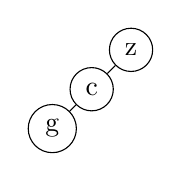
\begin{tikzpicture}[every node/.style={circle, draw, align=center}]
                    \node (z) at (0,0) {z};
                    \node (c) at (-.5,-.5) {c};
                    \node (g) at (-1,-1) {g};
                
                    \draw (z) -- (c);
                    \draw (c) -- (g);
                \end{tikzpicture} 
                \qquad u $\leftarrow$ rotate-right(z) \;
                \Return u \;
            }
            \Case{Double-right rotation}{
                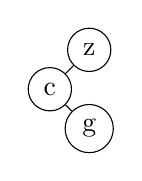
\begin{tikzpicture}[every node/.style={circle, draw, align=center}]
                    \node (z) at (0,0) {z};
                    \node (c) at (-.5,-.5) {c};
                    \node (g) at (0,-1) {g};
                
                    \draw (z) -- (c);
                    \draw (c) -- (g);
                \end{tikzpicture} 
                \qquad rotate-left(c); \qquad u $\leftarrow$ rotate-right(z) \;
                \Return u \;
            }
            \Case{Double-left rotation}{
                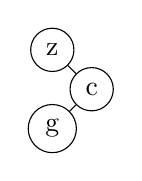
\begin{tikzpicture}[every node/.style={circle, draw, align=center}]
                    \node (z) at (0,0) {z};
                    \node (c) at (.5,-.5) {c};
                    \node (g) at (0,-1) {g};
                
                    \draw (z) -- (c);
                    \draw (c) -- (g);
                \end{tikzpicture} 
                \qquad rotate-right(c); \qquad u $\leftarrow$ rotate-left(z) \;
                \Return u \;
            }
            \Case{Left rotation}{
                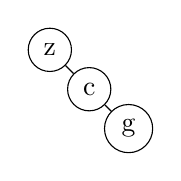
\begin{tikzpicture}[every node/.style={circle, draw, align=center}]
                    \node (z) at (0,0) {z};
                    \node (c) at (.5,-.5) {c};
                    \node (g) at (1,-1) {g};
                
                    \draw (z) -- (c);
                    \draw (c) -- (g);
                \end{tikzpicture} 
                \qquad u $\leftarrow$ rotate-left(z) \;
                \Return u \;
            }
        }
    }
\end{algorithm}

\subsection{Deletion in AVL Trees} 

\begin{algo}[].
    \begin{enumerate}
        \item Remove the key $k$ with \code{BST::delete}. 
        \item Find node where structural change happened. (This is not necessarily near the node that had $k$.) 
        \item Go back up to root, update heights, and rotate if needed. 
    \end{enumerate}
\end{algo}

\begin{codes}[].
    \begin{algorithm}[H]
        \caption{AVL Tree Deletion}
        \DontPrintSemicolon
        \KwIn{Key $k$ to delete}
        \KwOut{Updated AVL tree after deletion}
        
        $z \leftarrow \text{BST::delete}(k)$ \tcp*{leaf where $k$ was removed, assume $z$ is the parent of this node}
        \While{$z \neq \text{NULL}$}{
            \If{$\left| \text{z.left.height} - \text{z.right.height} \right| > 1$}{
                Let $c$ be the taller child of $z$ \;
                Let $g$ be the taller child of $c$ \tcp*{break ties to avoid double rotation}
                $z \leftarrow \text{restructure}(g, c, z)$ \;
                \textbf{break} \tcp*{can argue that we are done}
            }
            $\text{set-height-from-subtrees}(z)$ \;
            $z \leftarrow z.\text{parent}$ \;
        }
    \end{algorithm}
\end{codes}

\subsection{AVL Tree Summary}

\begin{enumerate}
    \item \textbf{search}: Just like in BSTs, costs $\Theta(height)$; 
    \item \textbf{insert}: \code{BST:insert}, then check \& update along path to new leaf. \begin{itemize}
        \item total cost: $\Theta(height)$; 
        \item restructure will be called at most once.
    \end{itemize}
    \item \textbf{delete}: \code{BST::delete}, then check \& update along path to deleted node \begin{itemize}
        \item total cost: $\Theta(height)$; 
        \item restructure may be called $\Theta(height)$ times. 
    \end{itemize}
\end{enumerate} 

\newpage

\section{Other Dictionary Implementations} 

\begin{thmm}[].
    We can show: If the KVPs were inserted in random order, then the expected height of the binary search tree would be $O(\log n)$. 
\end{thmm}

\subsection{Skip Lists} 

\begin{deff}[Skip List \index{Skip List}].
    A hierarchy L of ordered linked lists (levels) $L_0, L_1, \ldots, L_h$, 
    \begin{itemize}
        \item $L_0$ contains the KVPs of some $S$ in non-decreasing order; 
        \item For each of the subsequent levels, choose each item from previous level with probability $1/2$; 
        \item each $L_i$ also contains special keys (sentinels) $- \infty$ and $+ \infty$; 
        \item $L_h$ contains only sentinels, the left sentinel is the root.
    \end{itemize}
\end{deff}

\begin{discovery}[].
    Each list is a subsequence of previous one, i.e. 
    \[ L_0 \subseteq L_1 \subseteq \cdots \subseteq L_h \]
\end{discovery}

\begin{discovery}[].
    \begin{itemize}
        \item $i^{th}$ list is expected to have $n/2^i$ nodes; 
        \item Expect about $\log(n)$ lists in total. 
    \end{itemize}
\end{discovery}

\begin{examplee}[].
    \begin{center}
        \includegraphics[width=0.7\textwidth]{img/skip_list.png}
    \end{center}
\end{examplee}

\begin{deff}[Tower \index{Tower}].
    Each key $k$ belongs to a tower of nodes, and we define the \textbf{height of tower} for $k$ is the largest $i$ s.t. $k \in L_i$. 
\end{deff}

\begin{deff}[Height of Skip List \index{Height of Skip List}].
    Height of the skip list is the maximum height of any tower. 
    \begin{comm}[].
        Height is 3 in the above example. 
    \end{comm}
\end{deff}

\begin{codes}[].
    Each node $p$ has references to \code{after(p)} and \code{below(p)}. 
\end{codes}

\begin{examplee}[].
    \begin{center}
        \includegraphics[width=0.7\textwidth]{img/skip_list2.png}
    \end{center}
\end{examplee}

\subsubsection{Search in Skip Lists} 

\begin{algorithm}[H]
    \caption{getPredecessors}
    \SetAlgoLined
    \KwIn{Key $k$}
    \KwOut{Stack of nodes $P$ containing predecessors}
    $p \leftarrow \text{root}$\;
    $P \leftarrow \text{stack of nodes, initially containing } p$\;
    \While{$p.\text{below} \neq \text{NULL}$}{
        $p \leftarrow p.\text{below}$\;
        \While{$p.\text{after.key} < k$}{
            $p \leftarrow p.\text{after}$\;
        }
        $P.\text{push}(p)$\;
    }
    \Return{$P$}
\end{algorithm}

\begin{deff}[Predecessor \index{Predecessor}].
    For each level, predecessor of key $k$ is
    \begin{itemize}
        \item If key $k$ is present at the level: node before node with key $k$; 
        \item if key $k$ is not present at the level: node before node where $k$ would have been. 
    \end{itemize}
\end{deff}

\begin{algorithm}[H]
    \caption{skipList::search}
    \SetAlgoLined
    \KwIn{Key $k$}
    \KwOut{Node corresponding to key $k$ or location where $k$ would be}
    $P \leftarrow \text{getPredecessors}(k)$\;
    $q \leftarrow P.\text{top}()$\;
    \eIf{$q.\text{after.key} = k$}{
        \Return{$q.\text{after}$}
    }{
        \Return{``not found, but would be after $q$''}
    }
\end{algorithm}

\subsubsection{Insert in Skip List} 

\begin{codes}[].
    \begin{algorithm}[H]
        \SetAlgoLined
        \SetKwInOut{Input}{Input}
        \SetKwInOut{Output}{Output}
        \Input{Key $k$, Value $v$}
        \Output{Inserts the key-value pair $(k, v)$ into the skip list}
        \BlankLine
        $i \leftarrow 0$ \tcp*{\textcolor{orange}{initialize level counter}}
        \textbf{while} \textnormal{random}(2) = 1 \quad \textbf{do} $i \leftarrow i + 1$ \tcp*{\textcolor{orange}{random tower height} }
        $h \leftarrow 0$; $p \leftarrow \textnormal{root.below}$; \tcp*{\textcolor{orange}{start from the base level}}
        \textbf{for} ( $h \leftarrow 0$, $p \leftarrow root.below$; $p \neq NILL$; $p \leftarrow p.below$ ) \quad \textbf{do} $h++$ \;
        $P \leftarrow \textnormal{getPredecessors}(k)$\;
        $p \leftarrow P.\textnormal{pop}()$\;
        $zBelow \leftarrow$ new node with $(k, v)$ inserted after $p$ \tcp*{\textcolor{orange}{insert $(k, v)$ in $L_0$}}
        \While{$i > 0$}{
            $p \leftarrow P.\textnormal{pop}()$\;
            $z \leftarrow$ new node with $k$ added after $p$\;
            $z.\textnormal{below} \leftarrow zBelow$\;
            $zBelow \leftarrow z$\;
            $i \leftarrow i - 1$\;
        }
        \caption{Insertion in a Skip List}
    \end{algorithm}
\end{codes}

\subsubsection{Delete in Skip List} 

\begin{codes}[].
    \begin{algorithm}[H]
        \SetAlgoLined
        \SetKwInOut{Input}{Input}
        \SetKwInOut{Output}{Output}
        \Input{Key $k$ to be deleted}
        \Output{Deletes the key $k$ from the skip list}
        \BlankLine
        $P \leftarrow \textnormal{getPredecessors}(k)$ \tcp*{\textcolor{orange}{Find predecessors of $k$}}
        \While{$P$ is non-empty}{
            $p \leftarrow P.\textnormal{pop}()$ \tcp*{\textcolor{orange}{Get a predecessor of $k$ in some layer}}
            \textbf{if} $p.\textnormal{after}.key = k$ \quad \textbf{do} 
            $p.\textnormal{after} \leftarrow p.\textnormal{after}.\textnormal{after}$ \tcp*{\textcolor{orange}{Remove node}}
            \textbf{else} \textbf{break}
        }
        $p \leftarrow$ left sentinel of the root-list \tcp*{\textcolor{orange}{Move to root-list}} 
        \While{$p.\textnormal{below}.\textnormal{after}$ is the $\infty$ sentinel }{
            \tcp{\textcolor{orange}{The two top lists are both only sentinels, remove one}}
            $p.\textnormal{below} \leftarrow p.\textnormal{below}.\textnormal{below}$\;
            $p.\textnormal{after}.\textnormal{below} \leftarrow p.\textnormal{after}.\textnormal{below}.\textnormal{below}$\;
        }
        \caption{Deletion from a Skip List}
    \end{algorithm}
\end{codes}

\subsubsection{Skip List Analysis} 

Let $X_k$ be the height of tower for key $k$, we know $\displaystyle P(X_k \geq i) = \frac{1}{2^i}$. If $X_k \geq i$ then list $L_i$ includes key $k$.
Let $|L_i|$ be the number of keys in list $L_i$. Define $I_{i, k}$ as follows:
\[ I_{i, k} = \begin{cases} 
    0 & \text{if } X_k < i \\ 
    1 & \text{if } X_k \geq i 
\end{cases} \]
Then, the number of keys in list $L_i$ can be expressed as:
\[ |L_i| = \sum_{\text{key } k} I_{i, k} \]
The expected length of list $L_i$ is:
\[ E[|L_i|] = E\left[\sum_{\text{key } k} I_{i, k}\right] = \sum_{\text{key } k} E[I_{i, k}] = \sum_{\text{key } k} P(I_{i, k} = 1) = \sum_{\text{key } k} \frac{1}{2^i} = \frac{n}{2^i} \]

\begin{comm}[].
    Sentinels do not count towards the length; $L_0$ always contains all $n$ keys. 
\end{comm}

\begin{result}[].
    Thus, the expected length of list $S_i$ is $\frac{n}{2^i}$.
\end{result}

Also define 
\[ I_i = \begin{cases}
    0 & \text{if } |L_i| = 0 \\ 
    1 & \text{if } |L_i| \geq 1 
\end{cases} \]
Let $h = 1 + \sum_{i \geq 1} I_i$ (here $+1$ is for the sentinel-only level).

\begin{discovery}[].
    \begin{itemize}
        \item Since $I_i \leq 1$ we have that $E[I_i] \leq 1$.
        \item Since $I_i \leq |L_i|$ we have that $\displaystyle E[I_i] \leq E[|L_i|] = \frac{n}{2^i}$.
    \end{itemize}
\end{discovery}

\begin{comm}[].
    For ease of derivation, assume $n$ is a power of 2.
\end{comm}
\begin{align*}
    E[h] = E\left[ 1 + \sum_{i \geq 1} I_i \right] = 1 + \sum_{i \geq 1} E[I_i] 
    & = 1 + \sum_{i=1}^{\log n} E[I_i] + \sum_{i=1+\log n}^\infty E[I_i] \\
    & \leq 1 + \sum_{i=1}^{\log n} 1 + \sum_{i=1+\log n}^\infty \frac{n}{2^i} \\
    & = 1 + \log n + \frac{n}{2 \cdot 2^{\log n}} \sum_{i=0}^\infty \left(\frac{1}{2}\right)^i \\ 
    & = 1 + \log n + 1
\end{align*}

\begin{result}[].
    Expected skip list height $\leq 2 + \log n$. 
\end{result}

\paragraph{Skip List Analysis: Expected Space} We need space for nodes storing sentinels and nodes storing keys:

\begin{enumerate}
    \item \textit{Space for nodes storing sentinels}: 
    There are $2h + 2$ sentinels, where $h$ be the skip list height, recall that $E[h] \leq 2 + \log n$. Hence expected space for sentinels is at most:
    \[ E[2h + 2] = 2E[h] + 2 \leq 6 + 2\log n \]

    \item \textit{Space for nodes storing keys}: Let $|L_i|$ be the number of keys in list $L_i$, recall that $E[|L_i|] = \frac{n}{2^i}$. Hence expected space for keys is:
    \[ E\left[\sum_{i \geq 0} |L_i|\right] = \sum_{i \geq 0} E[|L_i|] = \sum_{i \geq 0} \frac{n}{2^i} = 2n \]
\end{enumerate}

\begin{result}[].
    Total expected space is $\Theta(n)$. 
\end{result}

\paragraph{Skip List Analysis: Expected Running Time} 

\begin{thmm}[].
    Total expected running time is $O(\log n)$. 
\end{thmm}

\begin{proof}
    \code{search}, \code{insert}, and \code{delete} are dominated by the runtime of \code{getPredecessors}. So we analyze the expected time of \code{getPredecessors}. We ‘drop-down’ $h$ times, where $h$ is skip list height, so the total expected time spent on ‘drop-down’ operations is $O(\log n)$. it now suffices to show that expected number of ‘scan-forward’ is also $O(\log n)$. 

    In general, in a random level $i$, the probability of scan-forward at least $l$ times is at most $(1/2)^l$. 
    \begin{comm}[].
        ‘at most’ because we could scan-down down. 
    \end{comm}
    Hence 
    \[ E[\text{\# scan-forward at level } i] = \sum_{l \geq 1} l \cdot P(\text{scans} = l) = \sum_{l \geq 1} P(\text{scans} \geq l) \leq \sum_{l \geq 1} \frac{1}{2^l} = 1 \]
    At level $i < h$: $E[\text{number of scan-forward}] \leq 1$. Also, expected number of scan-forward at level $i <$ number of keys at level $L_i$. Therefore \begin{align*}
        \sum_{i \geq 0} E[\text{\# of scan-forward at level } i] 
        & = \sum_{i=1}^{\log n} E[\text{\# of scan-for at level } i] + \sum_{i=1+\log n}^{\infty} E[\text{\# of scan-for at level } i] \\ 
        & \leq \sum_{i=1}^{\log n} 1 + \sum_{i=1+\log n}^{\infty} \frac{n}{2^i} \\
        & = \log n + 1
    \end{align*}
    Expected number of scan-forwards is $O(\log n)$.  
\end{proof}

\subsection{Biased Search Requests}

Unordered lists/arrays are among simplest data structures to implement but \code{search} is inefficient ($\Theta(n)$). 

\begin{Question}{}
    Can we make search in unordered lists/arrays more effective in practice?
\end{Question}

\begin{solution}
    No if items are accessed equally likely. Yes if the search requests are biased. 
\end{solution}

\subsubsection{optimal static ordering} 

\begin{Question}{}
    Scenario: We know access distribution, and want to find the best list order: \begin{center}
        \begin{tabular}{|l|c|c|c|c|c|}
            \hline
            \textit{Key}           
            & A  & B  & C  & D  & E  \\ \hline
            \textit{Frequency of Access} \qquad 
            & 2  & 8  & 1  & 10 & 5  \\ \hline
            \textit{Access Probability}   
            & \textcolor{red}{$2 / 26$} & \textcolor{green}{$8 / 26$} & \textcolor{blue}{$1 / 26$} & \textcolor{purple}{$10 / 26$} & \textcolor{orange}{$5 / 26$} \\ \hline
        \end{tabular}
    \end{center}
\end{Question}

\begin{deff}[ \index{}].
    Let the cost of search for key located at position \(i\) be \(i\).
    The expected cost of search, denoted as $T_{\text{exp}}(n)$, is given by: \begin{align*}
        T_{\text{exp}}(n) 
        & = \sum_{I \in I_n} T(I) \cdot \Pr(\text{randomly chosen instance } I) \\ 
        & = \sum_i i \cdot \Pr(\text{search for key at position } i) \\ 
        & = \sum_i i \cdot (\text{access probability for key at position } i)
    \end{align*}
\end{deff}

\begin{tcolorbox}[colback=yellow!10!white,colframe=orange]
    Ordering items by non-increasing access-probability minimizes expected access cost, i.e. best static ordering. 
\end{tcolorbox}

\subsubsection{dynamic ordering: MTF}

This time, we do not know the access probabilities ahead of time, so we modify the order dynamically, i.e. while we are accessing. 

\begin{comm}[].
    \hl{Rule of thumb: recently accessed item is likely to be accessed soon again} 
\end{comm}

\begin{deff}[MTF Heuristic \index{MTF Heuristic}].
    \textbf{Move-To-Front heuristic (MTF)}: after search, move the accessed  item to the front. 
\end{deff}

\begin{codes}[].
    Additionally, in list: always insert at the front. 
\end{codes}

\begin{thmm}[].
    Can show: MTF is ``2-competitive''. 
\end{thmm}

\newpage

\section{Dictionaries for special keys}

Realizations we have seen so far: \begin{itemize}
    \item Balanced Binary Search trees (AVL trees): $\Theta(\log n)$ \code{search}, \code{insert}, and \code{delete} (worst-case); 
    \item Skip lists: $\Theta(\log n)$ \code{search}, \code{insert}, and \code{delete} (expected). 
\end{itemize}
\hl{Various other realizations sometimes faster on insert, but search always takes $\Omega(\log n)$ time.} 

\begin{Question}{}
    Can one do better than $\Theta(\log n)$ time for search? 
\end{Question}

\begin{solution}
    It depends on what we allow: \begin{itemize}
        \item No: Comparison-based searching lower bound is $\Omega(\log n)$. 
        \item Yes: Non-comparison-based searching can achieve $o(\log n)$ (under restrictions!).
    \end{itemize}
\end{solution}

\subsection{Lower Bound for Comparison Based Algorithms} 

\begin{thmm}[].
    Any comparison-based algorithm requires in the worst case $\Omega(\log n)$ comparisons to search among $n$ distinct items.
\end{thmm}

\begin{proof}
    Via decision tree for items $x_0, \ldots, x_{n-1}$ and search for $k$. 
\end{proof}

\subsection{Interpolation Search}

Recall Binary Search, we always choose the middle point as out pivot point. But now, we have a more specific way of choosing such index: 

\begin{discovery}[].
    \[ \ell + \left\lceil \frac{ \overbrace{ k - A[\ell] }^{\text{distance from left key}} }{ \underbrace{ A[r] - A[\ell] }_{\text{distance between left and right keys}} } \times \underbrace{ (r - \ell - 1) }_{\text{\# unknown keys in range}} \right\rceil \]
\end{discovery}

\begin{codes}[].
    The following is the pseudocode for interpolating search algorithm. \\
    \begin{algorithm}[H]
        \DontPrintSemicolon % Removes the end of line semicolons
        \caption{Interpolation Search Algorithm}
    
        $\ell \gets 0$, \qquad $r \gets n - 1$\;
        \While{$\ell \leq r$}{
            \textbf{if} ($k < A[\ell]$ \textbf{or} $k > A[r]$), \textbf{then return} ``not found'' \;
            \textbf{if} $A[r] == k$, \textbf{then return} ``found at $A[r]$'' \;
            $m \gets \ell + \left\lceil \frac{k - A[\ell]}{A[r] - A[\ell]} \cdot (r - \ell - 1) \right\rceil$\;
            \textbf{if} ($A[m] == k$), \textbf{then return} ``found at $A[m]$'' \;
            \textbf{else if} ($A[m] < k$) \textbf{then} $\ell \gets m + 1$\;
            \textbf{else} $r \gets m - 1$\;
        }
    \end{algorithm}
\end{codes}

\begin{thmm}[].
    We can show that $T^{avg}(n) \leq T^{avg}(\sqrt{n}) + \Theta(1)$, which resolves to 
    \[ T^{avg}(n) \in O(\log \log n) \]
\end{thmm}

\begin{proof}
    This is difficult, specifically the recurrence relation part. 
\end{proof}

\subsection{Tries}  

Now we could have our keys as words instead of integers. 

\begin{deff}[Words (Strings) \index{Words (Strings)}].
    \textbf{Words} are sequences of characters over alphabet $\Sigma$. 
\end{deff}

\begin{codes}[].
    Conventioanlly, words have end-sentinel \$ (but it is sometimes not shown). 
\end{codes}

\begin{deff}[Size (of a word) \index{Size (of a word)}].
    The \textbf{size} of a word is the number of non-sentinel characters. 
    For instance, 
    \[ | helloworld\$ | = 10 \]
\end{deff}

\begin{comm}[].
    Words are sorted \texttt{lexicographically}. 
\end{comm}

\begin{deff}[Trie \index{Trie}].
    \begin{comm}[].
        Pronounced as ``try''. 
    \end{comm}
    \textbf{Trie} is also known as redix tree, it is a tree of bistrings based on bitwise comparisons whose edge are labelled with corresponding bit. 
\end{deff}

\begin{discovery}[].
    Due to end-sentinels, all key-value pairs are at leaves. 
\end{discovery}

\subsubsection{Trie: Search} 

\begin{algo}[].
    1. Follow links that corresponds to current bits in $w$. 2. Repeat until no such link or $w$ found at a leaf. \\ 
    \begin{algorithm}[H]
        \DontPrintSemicolon 
        \SetKwInOut{Output}{Output}
        \Output{Stack $P$ with all ancestors of where $w$ would be stored}
        \BlankLine
        
        $P \leftarrow$ empty stack; $z \leftarrow \text{root}$; $d \leftarrow 0$; $P.\text{push}(z)$\;
        \While{$d \leq |w|$}{
            \uIf{$z$ has a child-link labelled with $w[d]$}{
                $z \leftarrow \text{child at this link}$; \quad
                $d \leftarrow d + 1$; \quad 
                $P.\text{push}(z)$\;
            }
            \textbf{else} \textbf{break}
        }
        \Return{$P$}\;
        \caption{\code{Trie::get-path-to($w$)}}
    \end{algorithm}
    \begin{algorithm}[H]
        \DontPrintSemicolon 
        \BlankLine
        
        $P \leftarrow \text{get-path-to}(w)$; \quad $z \leftarrow P.\text{top}$\;
        \If{($z$ is not a leaf)}{
            \Return{``not found, would be in sub-trie of $z$''}\;
        }
        \Return{key-value pair at $z$}\;
        \caption{\code{Trie::search($w$)}}
    \end{algorithm}
\end{algo}

\subsubsection{Trie: Prefix-Search and Leaf Reference} 

We want another search-operation: 
\[ \code{prefix-search(w)} \] 
which find word $w'$ in trie for which $w$ is a prefix. 

\begin{algo}[].
    To find $w'$ quickly, we need leaf-references \begin{itemize}
        \item Every node $z$ stores reference $z.leaf$ to a leaf in subtree 
        \item \hl{Convention: store leaf with longest word}. 
    \end{itemize}
\end{algo}

\begin{codes}[].
    \begin{algorithm}[H]
        \DontPrintSemicolon 
        \BlankLine
        
        $P \leftarrow get\_path\_to(w)$ \;
        \If{(number of nodes on $P$ is $w.size$ or less)}{
            \Return{ ``no extension of $w$ found'' }
        } 
        \Return{P.top().leaf} 
        \caption{\code{Trie::prefix-search($w$)}}
    \end{algorithm}
\end{codes}

\subsubsection{Trie: Insert} 

\begin{algo}[].
    \begin{itemize}
        \item $P \leftarrow get\_path\_to(w)$ gives ancestors that exist already, 
        \item Expand the trie from $P.top()$ by adding necessary nodes that correspond to extra bits of $w$. 
        \item Update leaf-references (also at $P$ if $w$ is longer than previous leaves)
    \end{itemize}
\end{algo}

\subsubsection{Trie: Delete} 

\begin{algo}[].
    \begin{itemize}
        \item $P \leftarrow get\_path\_to(w)$ gives all ancestors. 
        \item Let $\ell$ be the leaf where $w$ is stored 
        \item Delete $\ell$ and nodes on $P$ until ancestor has two or more children. 
        \item Update leaf-references on rest of $P$. (If $z \in P$ referred to $\ell$, find new $z.leaf$ from other children.)
    \end{itemize}
\end{algo}

\subsubsection{Trie Summary} 

\begin{discovery}[].
    \code{search(w)}, \code{prefix-search(w)}, \code{insert(w)}, \code{delete(w)} all take time $\Theta (|w|)$. 
\end{discovery}

\begin{comm}[].
    Search-time is independent of number $n$ of words stored in the trie!
\end{comm}

\begin{result}[].
    The trie for a given set of words is unique (except for order of children and ties among leaf-references). 
\end{result}

\begin{discovery}[].
    Disadvantages: Tries can be wasteful with respect to space. Worst-case space is $\Theta (n \cdot (\text{maximum length of a word}))$. 
\end{discovery} 

\subsection{Variations of Tries: Pruned Tries} 

\begin{deff}[Pruned Trie \index{Pruned Trie}].
    Stop adding nodes to trie as soon as the key is unique. In other words, a node has a child only if it has at least two descendants.
\end{deff}

\begin{examplee}[].
    \begin{center}
        \includegraphics[width=0.75\textwidth]{img/pruned_trie.png}
    \end{center}
\end{examplee}

\begin{discovery}[].
    We have (implicitly) seen pruned tries before: For equal-length bitstrings: Pruned trie equals recursion tree of MSD radix-sort. 
\end{discovery}

\subsection{Variations of Tries: Compressed Tries} 

\begin{deff}[Compress Trie \index{Compress Trie}].
    Compress paths of nodes with only one child. Each node stores an index, corresponding to the level of the node in the uncompressed trie. (On level d, we searched for link with w[d].)
\end{deff}

\begin{comm}[].
    Compreesed Tries are also known as \textbf{Patricia-Tries}: \underline{P}ractical \underline{A}lgorithm to \underline{R}etrieve \underline{I}nformation \underline{C}oded in \underline{A}lphanumeric. 
\end{comm}

\begin{examplee}[].
    \begin{center}
        \includegraphics[width=0.6\textwidth]{img/compressed_trie.png}
    \end{center}
\end{examplee}

\begin{thmm}[].
    Compressed trie with $n$ keys has at most $n -1$ internal (non-leaf) nodes. 
\end{thmm}

\subsubsection{Compressed Trie: Search} 

\begin{comm}[].
    Stored indices say which bits to compare; 
    We must compare $w$ to word found at the leaf. 
\end{comm} 

\begin{codes}[].
    \begin{algorithm}[H]
        \DontPrintSemicolon 
        \BlankLine
        
        $P \leftarrow empty stack$; \quad $z \leftarrow root$; \quad $P.push(z)$ \; 
        \While {$z$ is not a leaf and ($d \leftarrow z.index \leq w.size$)}{
            \If {$z$ has a child-link labelled with $w[d]$} {
                $z \leftarrow \text{child at this link}$; \quad $P.push(z)$ 
            }
            \textbf{else break}; 
        }
        \Return{P}
        \caption{\code{CompressedTrie::get\_path\_to($w$)}}
    \end{algorithm}
    \begin{algorithm}[H]
        \DontPrintSemicolon 
        \BlankLine
        
        $P \leftarrow get\_path\_to(w)$, \quad $z \leftarrow P.top()$ \;
        \If{($z$ is not a leaf or word stored at $z$ is not $w$)}{
            \Return{ ``not found'' }
        } 
        \Return{key-value pair at $z$} 
        \caption{\code{CompressedTrie::search($w$)}}
    \end{algorithm}
\end{codes}

\subsubsection{Compressed Trie: Summary}

\begin{codes}[].
    \code{search} and \code{prefix-search} are easy. \code{insert(w)} and \code{delete(w)} are conceptually simple. 
\end{codes}

\begin{result}[].
    All operations take $O(|w|)$ time for word $w$. Use $O(n)$ space. 
\end{result}

\begin{comm}[].
    More complicated than standard tries, but space savings are worth it if words are unevenly distributed. 
\end{comm}

\subsection{Multiway Tries: Larger Alphabet} 

\begin{deff}[Multiway Trie \index{Multiway Trie}].
    \textbf{Multiway Trie} represents Strings over any fixed alphabet $\Sigma$. 
\end{deff}

\begin{discovery}[].
    Any node has at most $|\Sigma| + 1$ children, where $+1$ is the one child for the end-of-word character \$. 
\end{discovery}

\begin{examplee}[].
    A compressed trie holding strings $\{\text{bear}\$, \text{ben}\$, \text{be}\$, \text{soul}\$, \text{soup}\$\}$: \begin{center}
        \includegraphics[width=0.45\textwidth]{img/compressed_multiway.png}
    \end{center}
\end{examplee}

\begin{discovery}[].
    Run-time $O(|w| \cdot (\text{time to find the appropriate child}))$. 
\end{discovery}

\begin{Question}{}
    How should children be stored? 
\end{Question}

\begin{solution} 
    We have several options: 
    \begin{center}
        \includegraphics[width=0.9\textwidth]{img/store_children.png}
    \end{center} 
    However, \begin{result}[].
        Arrays are fast, lists are space efficient, AVL tree is best in theory, but not worth it in practice unless $|\Sigma|$ is huge. 
    \end{result}
\end{solution}

\begin{comm}[].
    In practice, use hashing (next section). 
\end{comm}

\newpage

\section{Midterm}

\begin{exer}[]. 
    \begin{cate}[Order Notation]. \end{cate}
    Prove from first principle that $n \in \omega( 2^{ \sqrt{\log n} } )$. 
\end{exer}

\begin{solution}
    Prove that 
    \[ 2^{\sqrt{ \log n }} \leq \sqrt{ n } \leq n \] 
    the rest follows easily. 
\end{solution}

\begin{exer}[]. 
    \begin{cate}[Order Notation]. \end{cate}
    Disprove the following statement: if $f(n) \in o(n \log n)$, then $f(n) \in O(n)$.
\end{exer}

\begin{solution}
    Take $f(n) = n \log \log n$. 
\end{solution}

\begin{exer}[]. \begin{cate}[Pseudocode Analysis]. \end{cate}
    Given a tight bound on the running time as a function on $n$ of the following pseudocode: 
    \begin{lstlisting}[language={}]
        i = 2
        x = 0
        while (i < n):
            for j = 1 to n:
                for k = 1 to j:
                    x = x + 1
            i = i * i
    \end{lstlisting}
\end{exer}
        
\begin{solution}
    We have $\lfloor \log \log n \rfloor$ iterations for the while loop, hence we have the tight bound: 
    \[ \sum_{y = 1}^{\log \log n} \sum_{j = 1}^n \sum_{k = 1}^j c \in \Theta (n^2 \log \log n) \] 
    as desired. 
\end{solution}

\begin{exer}[]. \begin{cate}[Expected Runtime]. \end{cate}
    Give a right big-$O$ bound for the expected runtime of the following algorithm: \begin{lstlisting}[language={}]
        ArrayAlg(A, n, k)
        // n = A.size()
        // A is a permutation of [0, ..., n-1]
        // k is in the set {0, ..., n-1}
        i = random(n)
        if A[i] == k then
            return i
        for j = 0 to n-1
            print("a")
        return ArrayAlg(A, n, k)
    \end{lstlisting}
\end{exer}

\begin{solution}
    Define $R = \langle i, R' \rangle$ and so we have 
    \[ T(A, R) = \begin{cases}
        c             & \text{ if } A[i] = k \\ 
        cn + T(A, R') & \text{ if } A[i] \neq k \\ 
    \end{cases} \]
    Hence solving for the expected runtime we get $T^{exp}(n) \in O(n^2)$. 
\end{solution}

\begin{exer}[]. \begin{cate}[Priority Queue]. \end{cate}
    Given a family $k$ sorted arrays $A_1, A_2, \ldots, A_k$, where the combination of the $k$ arrays has $n$ elements, provide an $O(n \log k)$ time algorithm that produces a single sorted array containing all $n$ elements. \textbf{Hint}: use a priority queue.
\end{exer}

\begin{solution}
    Create a min heap start with the first elements of all the $A_i$'s, keep deleting min and reinsert with the subsequent element in the corresponding $A_i$ to obtain the sorted array of length $n$. Each \code{deleteMin} and \code{insert} takes $\log k$ and there are $n$ of them so the total runtime is in $O(n \log k)$. 
\end{solution}

\begin{exer}[]. \begin{cate}[Epsilon]. \end{cate}
    Let $0 < \epsilon < 1$. Suppose that we have an array $A$ of $n$ items such that the first $n - n^\epsilon$ items are sorted. Describe an $O(n)$ time algorithm to sort $A$.
\end{exer}

\begin{solution}
    Merge sort the unsorted part, and then merge the originally sorted with the newly sorted. \\ 
    Merge sort the unsorted part takes $O(n^\varepsilon \log (n^\varepsilon))$, which can be shown to be in $O(n)$ using the fact that 
    \[ (\log n)^c \in o(n^d) \]
    for any $c$ and $d$ constants. Then it follows easily that merge takes linear time as well. 
    \begin{comm}[].
        The auxiliary space is also in $O(n)$. 
    \end{comm}
\end{solution}

\begin{exer}[]. \begin{cate}[Numbers in Range]. \end{cate}
    We have an array $A$ of $n$ non-negative integers such that each integer is less than $k$. Provide an $O(n + k)$ time preprocessing algorithm such that queries of the form "how many integers are there in $A$ that are in the range $[a, b]$?" can be answered in $O(1)$ time. Note that $a$ and $b$ are not fixed; they are parameters given to the query algorithm.
\end{exer} 

\begin{solution}
    First bucket sort to count the number of each integers, which takes $O(n+k)$, and then for each of the integer $\ell$, sum the number of integers in the range $[0, \ell]$, which takes $O(k)$, so that to find the number of intergers in $[a, b]$, we can just calculate $B[b] - B[a-1]$ in $O(1)$ times. 
\end{solution}

\begin{exer}[]. \begin{cate}[Binary Search and Interpolation Search]. \end{cate}
    T or F: Consider an algorithm that runs both Binary Search and Interpolation Search simultaneously until one of them stops. The worst-case runtime will be bounded by $O(\log n)$ and if the keys are uniformly distributed we would expect a runtime of $O(\log \log n)$.
\end{exer}

\begin{solution}
    True. 
\end{solution}

\begin{exer}[]. \begin{cate}[Heap]. \end{cate}
    Suppose heaps were implemented as trees (instead of arrays). Given two heaps $H_1$ and $H_2$ of the same height, a new heap can be created by building a new node with infinite priority and adding the root nodes of $H_1$ and $H_2$ as the left and right children, and then calling \texttt{deleteMax}.
\end{exer}

\begin{solution}
    False. 
\end{solution}

\newpage 

\section{Dictionaries via Hashing} 

Recall \textit{Direct Addressing}: Consider a special case where every key $k$ is integer with $0 \leq k < M$ for some $M \in \mathbb{N}$. The implementation for it is: 

\begin{algo}[].
    \begin{itemize}
        \item \code{store($k$,$v$)}: in array $A$ of size $M$ via $A[k] \leftarrow v$;  
        \item \code{search($k$)}: check if $A[k]$ is empty; 
        \item \code{insert($k$,$v$)}: $A[k] \leftarrow v$; 
        \item \code{delete($k$)}: $A[k] \leftarrow$ empty; 
    \end{itemize}
\end{algo}

\begin{discovery}[].
    Notice that all operations are $O(1)$, but total storage is $\Theta(M)$. 
\end{discovery}

\subsection{Hashing Introduction} 

\begin{deff}[Hashing (idea) \index{Hashing (idea)}].
    First map keys to small integer range and then use direct addressing. 
\end{deff}

\begin{comm}[].
    \textbf{Assumption}: keys come from some universe $U$. (Typically $U = \{0, 1, \ldots\}$, sometimes $U$ is finite.) 
\end{comm}

\begin{deff}[Hash Function \index{Hash Function}].
    We define \textbf{hash function} to be a function 
    \[ h : U \rightarrow \{0, 1, \ldots, M -1\} \] 
    and $h(k)$ is called \textbf{hash value} of $k$. \hl{Generally, hashing functions are not injective}. 

    \begin{examplee}[].
        For an instance: $h(k) = k \pmod{M}$. 
    \end{examplee}

    We store dictionary in array $T$ of size $M$ called \textbf{hash table}. 
\end{deff}

\begin{result}[].
    Hashing funcitions are fast ($O(1)$) to compute. 
\end{result}

\begin{discovery}[].
    However, as you might have noticed, collisions might happen. 
\end{discovery}

\begin{deff}[Collision \index{Collision}].
    \textbf{Collision} happens when we want to insert $(k, v)$, but $T[h(k)]$ is occupied. 
\end{deff}

\begin{algo}[].
    When collisions happen, there are two main strategies to deal with it: 
    \begin{itemize}
        \item \texttt{Chaining}: allow multiple items at each table location; 
        \item \texttt{Open addressing}: alternative slots in array: 
        \begin{itemize}
            \item probe sequence: many alternative locations \begin{itemize}
                \item linear probing 
                \item double hashing
            \end{itemize} 
            \item cuckoo hashing: just one alternative location
        \end{itemize}
    \end{itemize}
\end{algo}

\subsection{Hashing with Chaining} 

\begin{deff}[Bucket \index{Bucket}].
    Each slot is a \textbf{bucket} containing 0 or more KVPs. 
\end{deff}

\begin{deff}[Chaining \index{Chaining}].
    \textbf{Chaining} refers to the approach that makes each bucket an unsorted linked list. 
\end{deff}

\begin{codes}[Operations].
    \begin{itemize}
        \item \code{search($k$)}: look for key $k$ in the list at $T[h(k)]$; 
        \begin{comm}[].
            apply MTF heuristic. 
        \end{comm}
        \item \code{insert($k$, $v$)}: add $(k, v)$ to the front of list at $T[h(k)]$; 
        \item \code{delete($k$)}: search and delete from the list at $T[h(k)]$. 
    \end{itemize}
\end{codes}

\subsubsection{Hash with Chaining: Running Time} 

\begin{discovery}[].
    We have \begin{itemize}
        \item \code{insert}: $\Theta(1)$, essentially insertion of unordered linked list; 
        \item \code{search}, \code{delete}: $\Theta(1 + \text{length at } T[h(k)])$. \begin{comm}[].
            We don't say $\Theta(\text{length at } T[h(k)])$ because the length could be 0. 
        \end{comm}
    \end{itemize}
\end{discovery}

\begin{result}[].
    However, notice that the worst case could happen: $n$ keys are hashed at the same slot. 
\end{result}

\begin{comm}[].
    To get meaningful average-case bounds, we need some assumptions on hash function and key, but it's hard to make realistic assumptions. On the countrary, it's easier to switch to randomized hashing. 
\end{comm}

\paragraph{Hashing with Chaining: Randomization} 
\phantom{text} \\
\vspace{-0.25cm} 
\begin{Question}{}
    How can we randomize? 
\end{Question}

\begin{solution}
    Notice that we cannot insert at a random location, as key $k$ must hash to the hash value $h(k)$. Hence we assume hash-function is chosen randomly from a set of all hash functions. 
\end{solution}

\begin{thmm}[Uniform Hashing Assumption (UHA)].
    Any possible hash-function is equally likely to be chosen. \\
    (This is not realistic, but makes the analysis possible.) 
    \begin{comm}[].
        In practice: chose a random hash function from a certain family of hash functions. \begin{examplee}[].
            Pick prime number $p > M$ and random $a, b \in \{0, \ldots, p-1\}$ with $a \neq 0$, define  
            \[ h(k) = (ak + b \pmod{p}) \pmod{M} \]
        \end{examplee}
    \end{comm}
\end{thmm}

Notice that under UHA (any hash-function is chosen equally likely), we have 
\begin{enumerate}
    \item $\displaystyle P( h(k) = i ) = \frac{1}{M}$ for any key $k$ and slot $i$. \begin{proof}
        Let $k$, $i$ be some key and slot. Let $\mathcal{H}_j$ (for $j = 0, \ldots, M -1)$ be set of hash-functions $h$ s.t. $h(k) = j$. Hence for $j \neq i$, there exists an one-to-one map between $\mathcal{H}_j$ and $\mathcal{H}_i$. As a result, size of $\mathcal{H}_j$ is equal to $1 / M$ of all hash functions. 
    \end{proof}
    \item hash-values of any two keys are independent of each other. 
\end{enumerate}

\begin{result}[].
    (1) and (2) mean that the distribution of keys is not important, chance of two keys colliding is $1 / M$. 
\end{result}

\begin{deff}[Load Factor (Probe Sequence) \index{Load Factor (Probe Sequence)}].
    We define load factor, $\alpha$, to be $n / M$, where $n$ is the number of items and $M$ is the size of the hash table. 
\end{deff}

\begin{thmm}[].
    For any key $k$, the expected size of bucket $T[h(k)]$ is at most $1 + \alpha$. 
\end{thmm}

\begin{proof}
    Suppose $h(k) = i$, so we have two cases: \begin{enumerate}
        \item \textit{$k$ is not in the dictionary}: then each of the $n$ items in dictionary hashes to $i$ with probability of $1 / M$. Let $I_q^i = 1$ if key $q$ hashes to $i$ and $I_q^i = 0$ otherwise, so 
        \begin{align*}
            \mathbb{E}[ |T[i]| ] 
            = \mathbb{E} \left[ \sum_{\text{key } q} I_q^i \right] 
            = \sum_{\text{key } q} \mathbb{E} \left[ I_q^i \right] 
            = \frac{n}{M} \leq 1 + \alpha
        \end{align*}
        \item \textit{$k$ is in the dictionary}: $T[i]$ definitely has key $k$, and the remaining $n -1$ dictionary items hash to $i$ with probability $1 / M$. Hence 
        \begin{align*}
            \mathbb{E}[ |T[i]| ] = 1 + \frac{n - 1}{M} \leq 1 + \alpha
        \end{align*}
    \end{enumerate}
    thus we have completed our proof. 
\end{proof}

\begin{result}[].
    Expected runtime of \code{search} and \code{delete} is $\Theta(1 + \alpha)$, \code{insert} is $\Theta(1)$. Space is $\Theta(M + n)$. 
\end{result}

\begin{discovery}[].
    Therefore, if we could maintain $\alpha \in \Theta(1)$, we can have \code{search} and \code{delete} in constant time as well. 
\end{discovery}

\subsubsection{Load Factor and Rehashing}

\begin{algo}[].
    \begin{itemize}
        \item start with small $M$
        \item during \code{insert}/ \code{delete}, update $n$ 
        \item if load factor becomes too big, rehash \begin{itemize}
            \item chose new $M' \approx 2M$
            \item find a new random hash function $h'$ that maps $U$ into $\{0, 1, \ldots, M' -1\}$ 
            \item create new hash table $T'$ of size $M'$ 
            \item reinsert each KVP from $T$ into $T'$ 
            \item update $T \leftarrow T'$, $h \leftarrow h'$ 
        \end{itemize} 
        \item if load factor becomes too small, rehash with smaller $M'$. 
    \end{itemize}
\end{algo}

\begin{result}[].
    Rehashing costs $\Theta(M + n)$ but happens rarely, cost amortized over all operations. 
\end{result}

\subsection{Open Addressing} 

\subsubsection{Open Addressing}

Notice how chaining wastes space on links. 

\begin{Question}{}
    Can we resolve collisions in the array $H$?  
\end{Question}

\begin{solution}
    The idea is: each hash table entry holds only one item, but key $k$ can go in multiple locations. 
\end{solution}

\begin{deff}[Probe Sequence \index{Probe Sequence}].
    \code{search} and \code{insert} follow a \textbf{probe sequence} of possible locations for key $k$: 
    \[ h(k,0), h(k,1), h(k,2), \ldots \] 
    until an empty spot is found. 
\end{deff}

\begin{deff}[Linear Probing \index{Linear Probing}].
    \textbf{Linear probing} is the simplest method for probe sequence: If $h(k)$ is occupied, place item in the next available location. 
\end{deff}

\begin{comm}[].
    We assume circular array. i.e. modular arithmetic 
    \[ h(k, i) = h(k) + i \pmod{M} \] 
\end{comm}

\begin{discovery}[].
    Notice that if so, \code{delete} becomes problematic, because it would leave an empty spot which would make the next search not go far enough.
\end{discovery}

\begin{solution}
    To solve this, one approach is \textit{lazy deletion}: mark spot as deleted (rather than empty), and when perform searching, continue past deleted spots. Similarly, insert in empty or deleted spot. \\ 
    We also need to keep track of how many items are deleted and rehash if there are too many. 
\end{solution}

\subsubsection{Probe Sequence Operations} 

\begin{codes}[Insert]. 
    \begin{algorithm}[H]
        \textbf{probe-sequence::insert}($T, (k,v)$) 

        \For{$i = 0$ \textbf{to} $M-1$}{
            \If{$T[h(k,i)]$ is \textcolor{red}{empty} \textbf{or} \textcolor{red}{deleted}}{
                $T[h(k,i)] = (k, v)$ \;
                \Return \textbf{success} \;
            }
        }
        \Return \textbf{failure to insert}
    \end{algorithm}
\end{codes}

\begin{codes}[Delete].
    \begin{algorithm}[H]
        \textbf{probe-sequence::search}($T, k$) 

        \For{$i = 0$ \textbf{to} $M-1$}{
            \textbf{if} $T[h(k,i)]$ is \textcolor{red}{empty} \textbf{then} \Return item-not-found \;
            \textbf{if} $T[h(k,i)]$ has key $k$ \textbf{then}
            \Return $T[h(k,i)]$ \;
            \tcp{\textcolor{teal}{$T[h(k,i)]$ = deleted or not in the data structure therefore keep searching}}
        }
        \Return \textbf{item not found}
    \end{algorithm}
\end{codes}

\begin{result}[Drawbacks of linear probing].
    Entries tend to cluster into contiguous regions; Many probes for each \code{search}, \code{insert}, and \code{delete}. 
\end{result}

\subsubsection{Double Hashing} 

\begin{deff}[Double Hashing \index{Double Hashing}].
    \textbf{Double hashing}: open addressing with probe sequence: 
    \[ h(k, i) = h_0(k) + i \cdot h_1(k) \pmod{M} \qquad \text{for } i = 0, 1, \ldots \]
    Where \begin{itemize}
        \item $h_1$ is a secondary hash function (step size) s.t. $h_1(k) \neq 0$; 
        \item $h_1$ is relative prime with $M$ for all keys $k$ -- because otherwise probe-sequence does not explore the entire hash table. 
        \begin{comm}[].
            Easiest is to choose $M$ prime. 
        \end{comm}
    \end{itemize}
\end{deff}

\begin{thmm}[].
    Double hashing with a good secondary hash function does not cause the bad clustering produced by linear probing. 
\end{thmm}

\begin{discovery}[].
    We use multiplicative method for second hash function: \begin{itemize}
        \item let $0 < A < 1$; 
        \item $h(k) = M ( \underbrace{kA - \lfloor kA \rfloor}_{\in [0, 1)}$. 
    \end{itemize}
\end{discovery}

\begin{comm}[].
    Multiplying with $A$ scrambles the keys. We should use at least $\log|U| + \log|M|$ bits of $A$. 
\end{comm}

\begin{thmm}[].
    Taking $A = \varphi = \frac{\sqrt{5} - 1}{2}$ works well. For double hashing, to ensure $0 < h(k) < M$, use 
    \[ h_1(k) = \lfloor (M - 1) (kA - \lfloor kA \rfloor) \rfloor + 1 \]
\end{thmm}

\begin{examplee}[].
    \begin{minipage}{0.7\textwidth}
        Consider $M = 11, h_0(k) = k \mod 11, h_1(k) = \lfloor 10(\varphi k - \lfloor \varphi k \rfloor) \rfloor + 1$, and 
        \[ h(k,i) = (h_0(k) + i \cdot h_1(k)) \mod M \]
        for sequence $i = 0,1, \dots$. The table to the right demonstrate the cells we check when we try to perform 
        \[ \code{insert(194)} \]
        aside: $h_0(194) = 7$ and $h_1(194) = 9$, and \begin{align*}
            h(194, 0) & = 7 + 0 \cdot 9 \mod 11 = 7 \\ 
            h(194, 1) & = 7 + 1 \cdot 9 \mod 11 = 5 \\ 
            h(194, 2) & = 7 + 2 \cdot 9 \mod 11 = 3 
        \end{align*}
    \end{minipage} \begin{minipage}{0.25\textwidth}
        \begin{center}
            \begin{tabular}{!{\color{blue}\bfseries}c|c}
                \textbf{Index} & \textbf{Value} \\ \hline
                0  &  \\ \hline
                1  & 45 \\ \hline
                2  & 13 \\ \hline
                3  & \cellcolor{green!40} 194 \\ \hline
                4  & 92 \\ \hline
                5  & \cellcolor{red!60} 49 \\ \hline
                6  &  \\ \hline
                7  & \cellcolor{red!60} 7 \\ \hline
                8  & 41 \\ \hline
                9  &  \\ \hline
                10 & 43 \\ 
            \end{tabular}
        \end{center}
    \end{minipage}
\end{examplee}

\subsubsection{Cuckoo Hashing} 

The main idea of cuckoo hashing is that 
\begin{quote}
    An item with key $k$ can be only at $T_0[h_0(k)]$ or $T_1[h_1(k)]$. 
\end{quote}

\begin{center}
    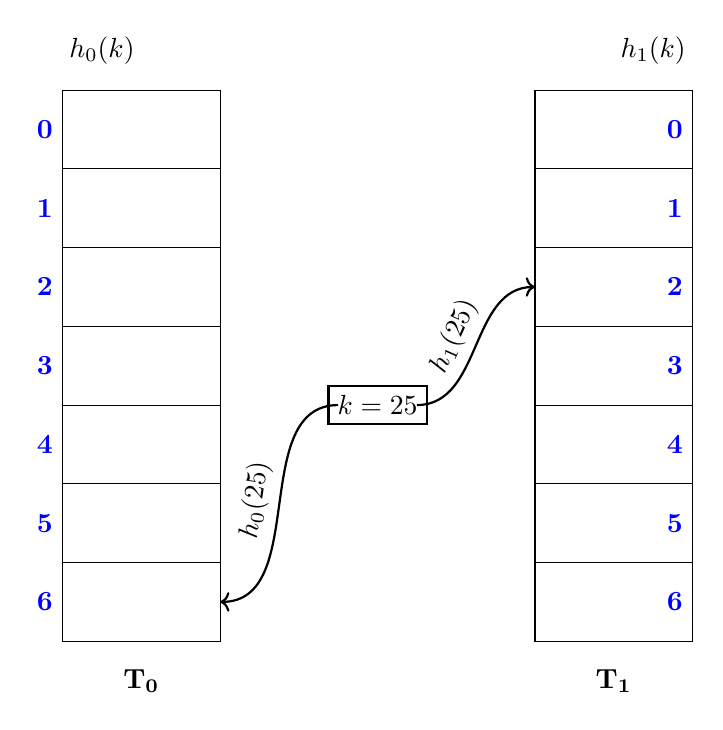
\begin{tikzpicture}

        % * Table for h_0(k)
        \node at (-3.5, 4.5) {\textbf{$h_0(k)$}};
        \draw (-4, -3) -- (-2, -3) -- (-2, 4) -- (-4, 4) -- cycle;
        \foreach \y in {-3,-2,-1,0,1,2,3}
            \draw (-4, \y) -- (-2, \y);
        \foreach \i in {0,1,2,3,4,5,6}
            \node[left, blue] at (-4, {3.5 - \i}) {\textbf{\i}};
    
        % * Table for h_1(k)
        \node at (3.5, 4.5) {\textbf{$h_1(k)$}};
        \draw (2, -3) -- (4, -3) -- (4, 4) -- (2, 4) -- cycle;
        \foreach \y in {-3,-2,-1,0,1,2,3}
            \draw (2, \y) -- (4, \y);
        \foreach \i in {0,1,2,3,4,5,6}
            \node[left, blue] at (4, {3.5 - \i}) {\textbf{\i}};
    
        % Box for k = 25
        \node[draw, thick] at (0, 0) {$k = 25$};
    
        % Arrows from k=25 to h0(k) and h1(k)
        \draw[->, thick] (0.5, 0) to[out=0, in=180] node[midway, above, sloped] {$h_1(25)$} (2, 1.5);
        \draw[->, thick] (-0.5, 0) to[out=180, in=0] node[midway, above, sloped] {$h_0(25)$} (-2, -2.5);
    
        \node at (-3, -3.5) {$\mathbf{T_0}$};
        \node at (3, -3.5) {$\mathbf{T_1}$};
    \end{tikzpicture}
\end{center}

\begin{discovery}[].
    \code{search} and \code{delete} take $O(1)$ time. 
\end{discovery}

\begin{algo}[].
    \code{insert} always initially puts key $k$ into $T_0[h_0(k)]$. 
    \begin{itemize}
        \item evict item that my have been there already 
        \item if so, evicted item $k'$ is inserted at $T_1[h_1(k')]$
        \item this may lead to a loop of evictions 
        \item we can show that if insertion is possible, \hl{then there are at most $2n$ evictions} 
        \item so we abort after too many attempts
    \end{itemize}
\end{algo}
    
\begin{codes}[].
    \begin{algorithm}[H]
        \caption{\textcolor{blue}{\textbf{cuckoo::insert}}$(k, v)$}
        $i \gets 0$\;
        \textbf{do} at most $2n$ times

        \Indp % Indent start
            \If{$T_i[h_i(k)]$ is empty} {
                $T_i[h_i(k)] \gets (k, v)$\;
                \Return \textbf{"success"}\;
            }
            \textcolor{teal}{// insert $T_i[h_i(k)]$ into the other table}\;
            \textcolor{blue}{\textbf{swap}}$((k, v), T_i[h_i(k)])$ \textcolor{teal}{// kick out current occupant}\;
            $i \gets 1 - i$ \textcolor{teal}{// alternate between 0 and 1}\;
        \Indm % Indent end
        
        \Return \textbf{failure} \textcolor{teal}{// re-hash}\;
    \end{algorithm}
    \begin{comm}[].
        Practical tip: we do not wait for $2n$ unsuccessful tries to declare failure. In practice, declare failure much earlier than $2n$. 
    \end{comm}
\end{codes}

\begin{deff}[Load Factor (cuckoo Hashing) \index{Load Factor (cuckoo Hashing)}].
    Load factor in cuckoo hashing is defined as 
    \[ \alpha = n \slash (\text{size of } T_0 + \text{size of } T_1) \]
\end{deff}

\begin{thmm}[].
    Can show that if the load factor is small enough, $\alpha < 1/2$, then insertion has $O(1)$ expected time. but this wastes space. 
\end{thmm}

\begin{thmm}[].
    Can show expected space is $O(n)$. 
\end{thmm}

\subsubsection{Running Time of Open Addressing Strategies} 

\begin{result}[].
    Under the restrictions of load factors and the Universal Hashing Assumption \begin{itemize}
        \item All strategies have $O(1)$ expected time for \code{search}, \code{insert}, \code{delete} 
        \item Cuckoo hashing has $O(1)$ worst case for \code{search}, \code{delete}  
        \item Probe sequence use $O(n)$ worst case space 
        \item Cuckoo hashing uses $O(n)$ expected space
    \end{itemize}
    For any hashing, the worst case runtime is $\Theta(n)$ for \code{insert}. 
\end{result}

\begin{comm}[].
    In practice, double hashing is the most popular, or cuckoo hashing if there are many more searches than insertions. 
\end{comm}

\subsection{Hash Function Strategies} 

Since satisfying the UHA is impossible, there are two ways to compromise: 
\begin{itemize}
    \item \textit{Deterministic}: hope for a good performance by choosing a hash function that is \begin{itemize}
        \item unrelated to any possible patterns in the data 
        \item Depends on all parts of the key
    \end{itemize}
    \item \textit{Randomized}: choose randomly among a limited set of functions, but aim for $P(\text{two keys collide}) = 1/M$. 
\end{itemize}

\subsubsection{Deterministic Hash Functions} 

\begin{algo}[].
    Randomized Hash Functiosn: Carter-Wegman’s Universal Hashing 
    \begin{itemize}
        \item Modular method; 
        \item Multiplicative method. 
    \end{itemize}
\end{algo}

\subsubsection{Randomized Hash Functiosn: Carter-Wegman’s Universal Hashing}

\begin{algo}[].
    \textbf{Requires:} all keys are in $\{0, \dots, p - 1\}$ for some (big) prime $p$. At initialization and whenever rehash
    \begin{itemize}
        \item choose number $M < p$, $M$ equal to some power of 2 is ok. 
        \item choose (and store) two \textcolor{red}{random} numbers $a, b \in \{0, \dots, p - 1\}$
        \begin{itemize}
            \item $b = \text{random}(p)$
            \item $a = 1 + \text{random}(p - 1)$, \textit{so that $a \neq 0$}
        \end{itemize}
        \item Use them as hash function
        \[ h(k) = ((ak + b) \mod p) \mod M \]
        \item can be computed quickly
    \end{itemize}
\end{algo}

\begin{thmm}[].
    We can prove that two keys collide with probability at most $\frac{1}{M}$
    \begin{comm}[].
        Enough to prove the expected runtime bounds for chaining, although uniform hashing assumption is not satisfied. 
    \end{comm}
\end{thmm}

\subsubsection{Multi-dimensional Data}

\begin{Question}{}
    What if the keys are multi-dimensional, such as strings? 
\end{Question}

\begin{solution}
    Standard approach is to \textcolor{red}{\textit{flatten}} string $w$ to integer $f(w) \in \mathbb{N}$, e.g.
    \begin{align*}
        \mathit{A \cdot P \cdot P \cdot L \cdot E} &\quad \rightarrow \quad (65, 80, 80, 76, 69) \quad \text{(ASCII)} \\
        &\quad \rightarrow \quad 65R^4 + 80R^3 + 80R^2 + 76R^1 + 69R^0 \\
        &\quad \text{(for some radix } R, \text{ e.g. } R = 255)
    \end{align*}
    We combine this with a modular hash function:
    \begin{align*}
        \boxed{ h(w) = f(w) \mod M }
    \end{align*}
\end{solution}

\begin{codes}[].
    To compute this in $O(|w|)$ time without overflow, use Horner’s rule and apply mod early. For example, $h(\mathit{APPLE})$ is
    \[ \left( \left( \left( \left( \left( \left( (65R + 80) \mod M \right) R + 80 \right) \mod M \right) R + 76 \right) \mod M \right) R + 69 \right) \mod M \]
\end{codes}

\subsection{Hashing vs. Balanced Search Trees}

\textbf{Advantages of Balanced Search Trees}
\begin{itemize}
    \item $O(\log n)$ worst-case operation cost
    \item does not require any assumptions, special functions, or known properties of input distribution
    \item predictable space usage (exactly $n$ nodes)
    \item never need to rebuild the entire structure
    \item supports ordered dictionary operations (rank, select, etc.)
\end{itemize}
\textbf{Advantages of Hash Tables}
\begin{itemize}
    \item $O(1)$ expected time operations (if hashes are well-spread and load factor is small)
    \item can choose space-time trade-off via load factor
    \item cuckoo hashing achieves $O(1)$ worst-case for search \& delete
\end{itemize}


\newpage

\section{Range-Searching in Dictionaries for Points} 

\subsection{Range Search}

\begin{deff}[Range Search \index{Range Search}].
    Operation \code{RangeSearch($x$, $x'$)} look for all items that fall within given range (interval) $Q = (x, x')$. 
    \begin{comm}[].
        $Q$ may have open or closed intervals. 
    \end{comm}
\end{deff}

As usual, $n$ is the number of input items, and let $s$ be the \textit{output-size}, i.e. the number of items in the range. We need $\Omega(s)$ time just to report the items in the range, where $s$ could be anything in $[0, n]$. Therefore, running time depends both on $s$ and $n$. It is easy to get $O(n)$ times. 

\begin{Question}{}
    Can we achieve $O(\log n + s)$? 
\end{Question}

\begin{solution}
    For unsorted list/array/hash table, we must check for each item explicitly if it is in the range, so range search requires $\omega(n)$ time. 

    For sorted array, we have: \begin{algo}[].
        \vspace{-.7cm}
        \item[\texttt{O(log n)}]: use binary search to find $i$ s.t. $x$ is at (or would be at) $A[i]$
        \item[\texttt{O(log n)}]: use binary search to find $i'$ s.t. $x'$ is at (or would be at) $A[i']$
        \item[\texttt{O(s)}]: report all items in $A[i + 1 \ldots i' - 1]$
        \item[\texttt{O(1)}]: report $A[i]$ and $A[i']$ if they are in the range
    \end{algo}
    hence range search can be done in $O(\log n + s)$ time. 

    For BST, range search can be done in $O(height + s)$ time, which will be proven later. 
\end{solution}

\subsection{Multi-Dimensional Data} 

\begin{comm}[].
    Range searches are of special interest for multidimensional data: flights that leave between 9am and noon, and cost between \$400 and \$600. 
\end{comm}

\subsubsection{Multi-Dimensional Range Search}

\begin{deff}[Multi-Dimensional Range Search \index{Multi-Dimensional Range Search}].
    (Orthogonal) $d$-dimensional range search is an operation such that given a query rectangle $Q$, it finds all points that lie within $Q$. 
\end{deff}

\subsubsection{$d$-Dimensional Dictionary via 1-Dimensional Dictionary} 

We have two options: 

\begin{algo}[].
    \begin{enumerate}
        \item Reduce to one-dimensional dictionary; 
        \item Use several dictionaries, one for each dimension. 
    \end{enumerate}
\end{algo}

\begin{codes}[Reduce to one-dimensional dictionary].
    We combine $d$-dimensional key into one dimensional key: i.e. 
    \[ (x, y) \mapsto x + y \cdot n^2 \]
    and hence two distinct $(x, y)$ map to a distinct one dimensional key. This way, we can search for a specific key, but no efficient range search. 
\end{codes}

\begin{codes}[ Use several dictionaries, one for each dimension].
    The problem with this is that it wastes space and leads to inefficient search. 
\end{codes}

\begin{examplee}[Worst case example].
    \begin{itemize}
        \item Insert all points into two dictionaries based on their x and y coordinates.
        \item Perform 1D range searches in both dictionaries, each returning half of the points.
        \item To find the intersecting points from both searches, insert the results from one dimension into an AVL tree and check for intersections with the other dimension.
        \item This method's complexity can approach $O(n \log n)$, worse than an exhaustive search ($O(s + \log n)$).
    \end{itemize}
\end{examplee}

\subsubsection{Multi-Dimensional Range Search (better idea)} 

\begin{discovery}[].
    We design new data structures specifically for points. 
\end{discovery}

\begin{comm}[].
    We assume that points are in general position: no two $x$-coordinates or $y$-coordinates are the same. i.e, no two points on a horizontal lines, no two points on a vertical line. 
\end{comm}

Here are the new data structure we design to help multidimensional search: 

\begin{result}[].
    \begin{enumerate}
        \item \texttt{Partition trees}: We will be studying two types of partition trees \begin{enumerate}
            \item quadtrees: does not use general points position assumption \item kd-trees: uses general points position assumption 
        \end{enumerate}
        
        \item \texttt{Multi-dimensional range trees}: a tree that generalizes BST to support multidimensional search whose both internal and leaf nodes store points just like similar to one dimensional BST. It uses general points position assumption
    \end{enumerate} 
\end{result}


\subsection{Quadtrees} 

Suppose we ave a set of points in the plane, we need to find a \textit{bounding box} $R = [0, 2^k) \times [0, 2^k)$ such that $R$ is the smallest $2^k \times 2^k$ square covers all the points. 

\begin{codes}[].
    keep subdividing regions (recursively) into smaller region until each region has at most one point. 
\end{codes}

\begin{examplee}[].
    \begin{center}
        \includegraphics[width=0.81\textwidth]{img/quadtree.png}
    \end{center}
\end{examplee}

\begin{comm}[].
    Convention: points on split lines belong to region on the right (or top).
\end{comm}

\subsubsection{\code{search}}

Analogous to trie or BST. 

\begin{codes}[].
    Three possibilities for where search ends \begin{enumerate}
        \item leaf storing point we search for (found) 
        \item leaf storing point different from search point (not found) 
        \item empty leaf (not found)
    \end{enumerate}
\end{codes}

\subsubsection{\code{insert}}

\begin{codes}[].
    \begin{enumerate}
        \item First perform search 
        \item Now we would have two cases: \begin{enumerate}
            \item search finds a leaf storing one point, then repeatedly split the leaf \textbf{while} there are two points in one region
            \item else if search finds an empty leaf, we then simply insert the point into leaf
        \end{enumerate}
        \item If we insert point outside the bounding box, no need to rebuild the part corresponding to the old tree, it becomes subtree in the new tree. 
    \end{enumerate}
\end{codes}

\subsubsection{\code{delete}}

\begin{codes}[].
    search will find a leaf containing the point, so we remove the point leaving the leaf empty, if parent now stores only one point in its region, we make parent node into a leaf storing its only child, and we check up the tree, repeating making any parent with only 1 point into a leaf. We do not make parent into a leaf as it stores multiple points. 
\end{codes}

\subsubsection{Quadtree Analysis} 

\begin{deff}[Spread Factor \index{Spread Factor}].
    We define \textbf{spread factor} $\rho(S)$ of points $S$ to be 
    \[ \rho(S) = \frac{L}{d_{min}} \]
    where $L$ is the side length of $R$ and $d_{min}$ is the minimum distance between two points in $S$. 
\end{deff}

\begin{thmm}[].
    In the worst case 
    \[ h \in \Omega( \log \rho(S)) \]
\end{thmm}

\begin{proof}
    While the smallest region diagonal is $\geq d_{min}$, there are two points in the same region, and if the height is $h$, we need to perform $h$ rounds of subdivisions. Notice that after this many subdivisions, the smallest region has side length of $L / 2^h$, and hence its diagonal is given by 
    \[ \sqrt{2} \cdot \frac{L}{2^h} \]
    recall that we want all the region to contain at most one points, hence we wish to have 
    \[ \sqrt{2} \cdot \frac{L}{2^h} < d_{min} \]
    which solves to be $h > \log ( \sqrt{2} \rho(S) )$. 
\end{proof}

\begin{thmm}[].
    In \textbf{any} case 
    \[ h \in O( \log \rho(S)) \]
\end{thmm}

\begin{proof}
    let be $v$ an internal node at depth $h-1$, so there are at least two points $p$ and $q$ in this region. Remember that $d_{min} \leq d(p, q)$, and the the corresponding region has side length $L / 2^{h-1}$. Recall taht the maximum distance between 2 points in such region is $\sqrt{2} \cdot L / 2^{h-1}$. Hence we have 
    \[ d_{min} \leq d(p, q) \leq \sqrt{2} \cdot \frac{L}{2^{h-1}} \]
    which gives us $h \leq 1 + \log( \sqrt{2} \rho(S) )$
\end{proof}

\begin{result}[].
    The complexity to build the initial tree is $\Theta(nh)$ worst case. 
\end{result}

\subsubsection{Quadtree Range Search}

\begin{codes}[].
    \begin{algorithm}[H]
        \SetAlgoLined
        \DontPrintSemicolon
        
        \caption{Quadtree Range Search Algorithm}
        \KwIn{$r \leftarrow \text{root}, Q \leftarrow \text{query rectangle}$}
        
        \SetKwFunction{FRangeSearch}{Qtree::RangeSearch}
        \SetKwProg{Fn}{Function}{:}{}
        \Fn{\FRangeSearch{$r$, $Q$}}{
            let $R$ be the region associated with $r$\;
            \uIf{$R \subseteq Q$}{
                report all points below $r$ \textbf{return}\;
            }
            \uElseIf{$R \cap Q = \emptyset$}{
                \textbf{return} \tcp*[r]{outside node, stop search}
            }
            \uIf{$r$ is a leaf}{
                $p \leftarrow$ point stored at $r$\;
                \textbf{if} $p$ is not NULL and in $Q$ \textbf{return} $p$ else \textbf{return}\;
            }
            \textbf{for} each child $v$ of $r$ \textbf{do} \FRangeSearch{$v$, $Q$}\;
        }
    \end{algorithm}
\end{codes}

\begin{discovery}[].
    Running time is number of visited nodes output size. We don't have a good bound on number of visited nodes. In the worst case, we may have to visit nearly all nodes in the worst case, hence $\Theta(nh)$ is the worst-case. 
    \begin{comm}[].
        In practice it is usually much faster. 
    \end{comm}
\end{discovery}

\subsubsection{Quadtree in Other Dimensions}

\begin{center}
    \begin{tabular}{|c|c|c|c|c|c|c|c|}
        \hline
        \rowcolor[HTML]{FFFFFF} 
        \cellcolor[HTML]{FFFFFF}points & \cellcolor[HTML]{A8CC70}0 & \cellcolor[HTML]{A8CC70}9 & \cellcolor[HTML]{A8CC70}12 & \cellcolor[HTML]{A8CC70}14 & \cellcolor[HTML]{ADD8E6}24 & \cellcolor[HTML]{ADD8E6}26 & \cellcolor[HTML]{ADD8E6}28 \\ \hline
        \rowcolor[HTML]{FFFFFF} 
        \cellcolor[HTML]{FFFFFF}base 2 & \cellcolor[HTML]{A8CC70}00000 & \cellcolor[HTML]{A8CC70}01001 & \cellcolor[HTML]{A8CC70}01100 & \cellcolor[HTML]{A8CC70}01110 & \cellcolor[HTML]{ADD8E6}11000 & \cellcolor[HTML]{ADD8E6}11010 & \cellcolor[HTML]{ADD8E6}11100 \\ \hline
    \end{tabular}
    \includegraphics[width=0.8\textwidth]{img/quadtree(otherdim).png}
\end{center}

\subsection{kd-Trees} 

Since quad trees can be extremely unbalanced, so we wish to introduce something new: kd-tree. 

\begin{deff}[kd-Tree \index{kd-Tree}].
    For kd-Trees, we contruct by splitting into regions with equal number of points, note that we can split either vertically or horizontally. 
    \begin{comm}[].
        Alternating vertical and horizontal splits gives range search efficiency. 
    \end{comm}
\end{deff}

\subsubsection{kd-tree Construction Running Time and Space} 

The expected time for partitioning $S$ is $\Theta(n)$ with \code{QuickSelect}. Both subtrees have $\approx n/2$ points. Hence we have the following sloppy recurrence: 

\begin{thmm}[].
    We have 
    \[ T^{exp}(n) = 2 T^{exp} \left( \frac{n}{2} \right) + O(n) \]
    which resolves to be $\Theta(n \log n)$ expected time. 
\end{thmm}

\begin{comm}[].
    We can improve the above to $\Theta(n \log n)$ worst-case runtime by pre-sorting coordinates. 
\end{comm}

\begin{thmm}[].
    In terms of the height, we have the following recurrence relation: 
    \[ h(0) = 1 \qquad \text{ and } \qquad h(n) \leq h \left( \left\lceil \frac{n}{2} \right\rceil \right) + 1 \]
    which resolves to $O(\log n)$, specifically, $\lceil \log n \rceil$. 
\end{thmm}

\begin{comm}[].
    The above bound is tight. 
\end{comm}

\begin{thmm}[].
    In terms of the space, all interior nodes have exactly 2 children, therefore there are $n-1$ interior nodes, and hence the total number of nodes is $2n - 1$. Hence space is $\Theta(n)$. 
\end{thmm}

\subsubsection{kd-tree Dictionary Operations} 

\begin{codes}[].
    \begin{enumerate}
        \item[\code{search}] as in binary search tree using indicated  coordinate 
        \item[\code{insert}] first search, insert as new leaf 
        \item[\code{delete}] first search, remove leaf and  any parent with one child
    \end{enumerate}
\end{codes}

\begin{Question}{}
    Notice that there are several problems with kd-Tree operations: 
    \begin{itemize}
        \item after insert or delete, split might no longer be at exact median 
        \item height is no longer guaranteed to be 
        \item kd-tree do not handle insertion/delection well
    \end{itemize}
\end{Question}

\begin{solution}
    Remidy: allow a certain imbalance; re-building the entire tree when it becomes too unbalanced; However, \code{rangeSearch} will be slower. 
\end{solution}

\subsubsection{kd-Tree Range Search}

\begin{codes}[].
    \begin{algorithm}[H]
        \caption{\textit{kdTree::RangeSearch}($r \leftarrow root, Q$)}
        \KwIn{$r$ : root of kd-tree, $Q$ : query rectangle}
        $R \gets$ region associated with node $r$ \;
        \If{ \textcolor{teal}{$R \subseteq Q$} }{
            report all points below $r$ \;
            \textbf{return} \;
        }
        \textbf{if} \textcolor{red}{$R \cap Q = \emptyset$} \textbf{return}\;
        \If{ \textcolor{blue}{$r$ is a leaf }}{
            $p \gets$ point stored at $r$ \;
            \textbf{if} $p \in Q$ \Return $p$ \;
            \textbf{else} \Return
        }
        \ForEach{ \textcolor{blue}{child $v$ of $r$} }{
            \textit{kdTree::RangeSearch}($v, Q$) \;
        }
    \end{algorithm}
\end{codes}

\subsubsection{kd-tree: Range Search Running Time} 

We visit \textcolor{blue}{blue}, \textcolor{red}{red}, and \textcolor{teal}{green} nodes, where there is constant work at each node. Hence runtime is proportional to the number of blue, red, green nodes. 

\paragraph{\textcolor{teal}{Green Nodes:}}

Recall that $s$ is the number of nodes in the output of range search, so there are at most $s$ leaves over all green subtrees, and, therefore, at most $2s$ nodes over all green subtrees. Hence 
\begin{thmm}[].
    Number of \textcolor{teal}{green} nodes is $O(s)$. 
\end{thmm}

\begin{discovery}[].
    Notice that \textcolor{red}{red nodes} $\leq 2 \cdot$ \textcolor{blue}{blue nodes} since each red node has a blue parent. Hence it is enough to count the number of blue nodes.  
\end{discovery}

\paragraph{\textcolor{blue}{Blue Nodes:}} Let $B(n)$ to be the number of blue nodes. 

\begin{thmm}[].
    We can show that 
    \[ B(n) \leq 2 B \left( \frac{n}{4} \right) + O(1) \]
    which can be resolved to $B(n) \in O(\sqrt{n})$. 
\end{thmm}

\begin{proof}
    We have 

    \begin{minipage}{0.5\textwidth}
        \begin{align*}
            B(n) \leq 
            & \text{\# regions intersecting } \textcolor{blue}{\textbf{|}}\\ 
            & \text{\# regions intersecting } \textcolor{teal}{\textbf{|}}\\ 
            & \text{\# regions intersecting } \textcolor{magenta}{\textbf{|}} \\ 
            & \text{\# regions intersecting } \textcolor{orange}{\textbf{|}} \\ 
        \end{align*}
        We consider \# regions intersecting \textcolor{blue}{\textbf{|}}, and so the other cases can be handled similarly. 
    \end{minipage} \begin{minipage}{0.4\textwidth}
        \begin{center}
            \includegraphics[width=0.8\textwidth]{img/kdTreeProof.png}
        \end{center}
    \end{minipage}

    Define $B^x(n)$ to be 
    \[ B^x(n) := \text{\# of regions intersecting } \textcolor{blue}{\textbf{|}} \]
    if tree root is splitted by $x$ coordinate. Hence we have 
    \[ B^x(n) = 1 + B^y \left( \frac{n}{4} \right) \]
    where $\displaystyle B^y \left( \frac{n}{2} \right) = 1 + 2 \cdot B^x \left( \frac{n}{4} \right)$. Combining them we get our desired result. 
\end{proof}

\begin{result}[].
    Therefore, the running time for range search is 
    \[ O(s + \sqrt{n}) \]
\end{result}

\subsubsection{kd-Tree | Higher Dimension} 

Consider a kd-Tree for $d$-dimensional space, we have \begin{center}
    \begin{tabular}{rcl}
        \texttt{storage} & : & $O(n)$; \\ 
        \texttt{height} & : & $O(\log n)$; \\ 
        \texttt{Construction Time} & : & $O(n \log n)$; \\ 
        \texttt{Range query time} & : & $\displaystyle O \left( s + n^{1 - 1/d} \right), \quad \text{where we assume $d$ is a constant}$.  
    \end{tabular}    
\end{center}

\subsection{Range Trees}

\begin{Question}{}
    Our question is: can we use ideas from BST/AVL trees for multi dimensional dictionaries? 
\end{Question}

\subsubsection{BST Range Search} 

\begin{examplee}[].
    First let us consider range search in BST: 
    \[ \code{ BST::RangeSearch(T, 28, 43) } \] 
    where $T$ is: \begin{center}
        \includegraphics[width=0.8\textwidth]{img/bstRangeSearch.png}
    \end{center}
    Notice that we have the following three types of nodes: \begin{itemize}
        \item \textcolor{blue}{Boundary nodes}: nodes on $P_1$ and $P_2$. We need to check if boundary nodes are in the search range.  
        \item \textcolor{red}{Outside nodes}: nodes that are left of $P_1$ or right of $P_2$, in this case, nodes are not in search range so range search never examines them. 
        \item \textcolor{teal}{Inside nodes}: nodes that are right of $P_1$ and left of $P_2$, so we keep a list of topmost inside nodes, and all descendants of topmost inside node are in the range, so we just report them. 
    \end{itemize}
\end{examplee}

\subsubsection{How to Find Top Inside Node} 

\begin{thmm}[].
    A node $v$ is a \textcolor{teal}{top inside node} if: \begin{itemize}
        \item $v$ is not in $P_1$ or $P_2$; 
        \item parent of $v$ is in $P_1$ or $P_2$ (but not both) 
        \begin{itemize}
            \item If parent is in $P_1$, then $v$ should be the right child of it, otherwise left child. 
        \end{itemize} 
    \end{itemize}
\end{thmm}

\begin{comm}[].
    Top inside nodes are important for efficient 2D range search, they are also important if need to just count the number of points in the search range. 
\end{comm}

\subsubsection{BST Range Search Analysis} 

\begin{comm}[].
    We assumed that we have balanced BST. 
\end{comm}

Running time consists of
\begin{enumerate}
    \item search for path \textbf{\textcolor{blue}{$P_1$}} is $O(\log n)$
    \item search for path \textbf{\textcolor{blue}{$P_2$}} is $O(\log n)$
    \item check if boundary nodes in the range
    \begin{itemize}
        \item $O(1)$ at each \textbf{\textcolor{blue}{boundary node}}, there are $O(\log n)$ of them, $O(\log n)$ total time
    \end{itemize}
    \item spend $O(1)$ at each topmost inside node
    \begin{itemize}
        \item since each topmost inside node is a child of boundary node, there are at most $O(\log n)$ topmost inside nodes, so total time $O(\log n)$
    \end{itemize}
    \item report descendants in subtrees of all topmost inside nodes
    \begin{itemize}
        \item topmost nodes are disjoint, so \#descendants for inside topmost nodes is at most $s$, output size
    \end{itemize}
\end{enumerate}

\begin{result}[].
    Hence total time is $O(s + \log n)$. 
\end{result}

\subsubsection{2D Range Tree}

\begin{deff}[2D Range Tree \index{2D Range Tree}].
    Suppose we have points: $S = \{(x_0, y_0), (x_1, y_1), \dots, (x_{n-1}, y_{n-1})\}$. \textbf{Range tree} is a \textcolor{red}{tree of trees} (a \textit{multi-level} data structure) \begin{itemize}
        \item \textcolor{red}{\textbf{Primary structure}}
        \begin{itemize}
            \item balanced BST $T$ storing $S$ and uses \textcolor{red}{$x$-coordinates} as keys
            \item assume $T$ is balanced, so height is $O(\log n)$
        \end{itemize}
        \item Each node $v$ of $T$ stores an \textcolor{red}{associated tree} $T(v)$, which is a balanced BST
        \begin{itemize}
            \item let $S(v)$ be all descendants of $v$ in $T$, including $v$
            \item $T(v)$ stores $S(v)$ in BST, using \textcolor{red}{$y$-coordinates} as key
            \begin{itemize}
                \item note that $v$ is not necessarily the root of $T(v)$
            \end{itemize}
        \end{itemize}
    \end{itemize}
\end{deff}

\begin{algo}[Range search in 2D Range Tree Overview].
    Suppose we want to perform \code{RangeTree::RangeSearch(T, \textcolor{teal}{5}, \textcolor{teal}{14}, \textcolor{blue}{5}, \textcolor{blue}{9})}, we wish to perform the following: \begin{enumerate}
        \item Perform \textit{modified} \textbf{BST-RangeSearch}$(T, \textcolor{teal}{5}, \textcolor{teal}{14})$
        \begin{itemize}
            \item find boundary and topmost inside nodes, but \textbf{\textcolor{red}{do not}} go through the inside subtrees
            \item modified version takes $ O(\log n) $ time
            \begin{itemize}
                \item does not visit all the nodes in valid range for \textit{BST-RangeSearch}$(T, \textcolor{teal}{5}, \textcolor{teal}{14})$
            \end{itemize}
        \end{itemize}
        
        \item Check if boundary nodes have valid $ x $-coordinate \textbf{and} valid $ y $-coordinate
        
        \item For every topmost inside node $ v $, search in associated tree \textit{BST::RangeSearch}$\big( T(v), \textcolor{blue}{5}, \textcolor{blue}{9} \big)$
    
    \end{enumerate}
\end{algo}

\subsubsection{Range Tree Space and Time Analysis}

\begin{center}
    \includegraphics[width=0.70\textwidth]{img/RangeTreeSpace.png}
\end{center}
\begin{center}
    \includegraphics[width=0.70\textwidth]{img/RangeTreeTime.png}
\end{center}

\begin{result}[].
    Range trees can be generalized to d -dimensional space: \begin{center}
        \begin{tabular}{rcl}
            \texttt{storage} & : & $O(n ( \log n )^{d-1})$; \\ 
            \texttt{Construction Time} & : & $O(n ( \log n )^d)$; \\ 
            \texttt{Range query time} & : & $\displaystyle O \left( s + ( \log n )^d \right)$ 
        \end{tabular}    
    \end{center} 
\end{result}


\subsection{Conclusion}

\paragraph{Quadtrees}
\begin{itemize}
    \item simple, easy to implement insert/delete (i.e. dynamic set of points)
    \item work well only if points evenly distributed
    \item wastes space, especially for higher than two dimensions
\end{itemize}

\paragraph{kd-trees}
\begin{itemize}
    \item linear space
    \item range search is $O(s + \sqrt{n})$
    \item inserts/deletes destroy balance and range search time
    \begin{itemize}
        \item fix with occasional rebuilt
    \end{itemize}
\end{itemize}

\paragraph{Range trees}
\begin{itemize}
    \item fastest range search $O(\log^2 n + s)$
    \item wastes some space
    \item insert and delete destroy balance, but can fix this with occasional rebuilt
\end{itemize}



\newpage

\section{String Matching} 

\begin{deff}[String Matching \index{String Matching}].
    The problem is about searching for a string (pattern) in a large body of text. Here are some of the notations: \begin{enumerate}
        \item $T[0, \ldots, n - 1]$: text (or haystack) being searched; 
        \item $P[0, \ldots, m - 1]$: pattern (or needle) being searched for. 
    \end{enumerate}
    \begin{comm}[].
        Convention: return the first occurrence of $P$ in $T$. 
    \end{comm}
\end{deff}

\[ \textbf{\textcolor{black}{anti}}\textbf{\textcolor{blue}{dis}}\textbf{\textcolor{red}{establish}}\textbf{\textcolor{black}{mentarian}}\textbf{\textcolor{teal}{ism}} \]

\begin{itemize}
    \item \begin{deff}[Substring \index{Substring}].
        \textbf{\textcolor{red}{Substring}} $T[i \dots j]$ \quad $0 \leq i \leq j + 1 \leq n$ is a string $T[i], T[i+1], \dots, T[j]$
        \begin{itemize}
            \item length is $j - i + 1$
            \item empty string included: $T[i \dots i - 1]$
        \end{itemize}
    \end{deff} 
    
    \item \begin{deff}[Prefix \index{Prefix}].
        \textbf{\textcolor{blue}{Prefix}} of $T$ is a substring $T[0 \dots i - 1]$ of $T$ for some $0 \leq i \leq n$
        \begin{itemize}
            \item empty prefix included: $T[0 \dots -1]$
        \end{itemize}
    \end{deff} 
    
    \item \begin{deff}[Suffix \index{Suffix}].
        \textbf{\textcolor{teal}{Suffix}} of $T$ is a substring $T[i \dots n-1]$ of $T$ for some $0 \leq i \leq n$
        \begin{itemize}
            \item empty suffix included: $T[n \dots n-1]$
        \end{itemize}
    \end{deff} 

    \item \begin{deff}[Empty String \index{Empty String}].
        The \textbf{empty substring} is usually denoted by $\Lambda$
    \end{deff}
\end{itemize}

\subsection{Introduction}

\begin{algo}[].
    Pattern matching algorithms consist of \textit{guesses} and \textit{checks}.  
\end{algo}

\begin{deff}[Guess \index{Guess}].
    A \textbf{guess} is a position $i$ such that $P$ might start at $T[i]$. 
\end{deff}

\begin{deff}[Check \index{Check}].
    A \textbf{check} of a guess is a single position $j$ with $0 \leq j < m$ where we compare $T[i + j]$ to $P[j]$. \begin{comm}[].
        Note that \begin{itemize}
            \item must perform $m$ checks of a single correct guess; 
            \item may make fewer checks of an incorrect guess. 
        \end{itemize}
    \end{comm}
\end{deff}

\subsection{Brute Force Algorithm} 

\begin{codes}[].
    \begin{lstlisting}[style=cppstyle]
        Bruteforce::PatternMatching(T [0..n - 1], P[0..m - 1])
        T : String of length n (text), P : String of length m (pattern)
        
        for i <- 0 to n - m do
            if strcmp(T, P, i, m) = 0
                return "found at guess i"
        return FAIL
    \end{lstlisting}
    where \code{strcmp} takes $\Theta(m)$ time. 
    \begin{lstlisting}[style=cppstyle]
        strcmp(T, P, i <- 0, m <- P.size())
        // compare m chars of T and P, starting at T[i]
        
        for j <- 0 to m - 1 do
            if T[i + j] is before P[j] in (*@$\Sigma$@*) then return -1
            if T[i + j] is after P[j] in (*@$\Sigma$@*) then return 1
        return 0
    \end{lstlisting}
\end{codes}

\begin{examplee}[Worst Possible Imput].
    Worst possible input is 
    \[ P = \underbrace{a \ldots a}_{m - 1 \text{ terms}} b, \qquad T = \underbrace{aaa \ldots aaa}_{n \text{ terms}} \] 
    Since we perform $(n - m + 1)m$ checks, the time is $\Theta( (n - m)m )$.
\end{examplee}

\begin{Question}{}
    How can we improve? 
\end{Question}

\begin{solution}
    Improvement via Preprocesing. There are two preprocessing options for pattern matching \begin{enumerate}
        \item Do preprocessing on pattern $P$, eliminate guesses based on preprocessing: \begin{itemize}
            \item Karp-Rabin \item KMP \item Boyer-Moore 
        \end{itemize}
        \item Do preprocessing on text $T$, create a data structure to find matches easily: \begin{itemize}
            \item Suffix-tree \item Suffix-arrays
        \end{itemize}
    \end{enumerate}
\end{solution}

\subsection{Karp-Rabin Algorithm} 

The idea is 
\[ \text{ use hash values (called \textbf{fingerprints}) to eliminate guesses } \]
where hash function $h : \{ \text{string of length $m$} \} \rightarrow \{0, \ldots, M - 1\}$. 

\begin{comm}[].
    if $h(P) \neq h(guess)$ then guess cannot work; if $h(P) = h(guess)$ verify with strcmp if pattern matches text. 
\end{comm}

\begin{examplee}[].
    Example: $\Sigma = \{0 - 9\}$, $P = 9 2 6 5 3$, $T = 3 1 4 1 5 9 2 6 5 3 5$: Precompute: 
    \[ h(P) = h(9 2 6 5 3) = 18 \]
    and we have the following table showing the process: 
    \begin{center}
        \begin{tabular}{l|c|c|c|c|c|c|c|c|c|c|c|c|l}
            \hline
            & 3 & 1 & 4 & 1 & 5 & 9 & 2 & 6 & 5 & 3 & 5 & \\ \hline
            \code{no strcmp} & \multicolumn{5}{|c|}{fingerprint 84} & & & & & & & 
            h(31415) = 84 \\ \hline
            \code{no strcmp} & & \multicolumn{5}{|c|}{fingerprint 94} & & & & & & 
            h(14159) = 94 \\ \hline
            \code{no strcmp} & & & \multicolumn{5}{|c|}{fingerprint 76} & & & & & 
            h(41592) = 76 \\ \hline
            \code{do strcmp}, false & & & & \multicolumn{5}{|c|}{fingerprint 18} & & & & 
            h(15926) = 18 \\ \hline
            \code{no strcmp} & & & & & \multicolumn{5}{|c|}{fingerprint 95} & & & 
            h(59265) = 95 \\ \hline
            \code{do strcmp}, true & & & & & & \multicolumn{5}{|c|}{fingerprint 18} & & 
            h(92653) = 18 \\ \hline
        \end{tabular}
    \end{center}
\end{examplee}

\begin{discovery}[].
    For each guess, we need $\Theta(m)$ time to compute hash value. Note that this method is thus worse than brute force, as the total time now is 
    \[ \Theta( m n ) \]
    How can we improve this? 
\end{discovery}

\begin{solution}
    \hl{compute next hash from previous one in $O(1)$ time.}
\end{solution}

\begin{examplee}[].
    Consider 
    \[ T = \textcolor{red}{ 4 \; 1 \; 5 \; 9 \; 2 } \; 6 \; 5 \; 3 \; 5 \]
    The initialization of the algorithm is: \begin{enumerate}
        \item compute first fingerprint: $h(41592) = 41592 \mod 97 = 76$ 
        \item also pre-compute $T^{m - 1} \mod M$ (here is $10000 \mod 97 = 9)$. 
    \end{enumerate}
    Down below is an example showing how we can get $h(15926)$ from $h(41592)$ in $O(1)$ time. 
    \[
        \textcolor{red}{4}1592 \quad
        \stackrel{ -\textcolor{red}{4} \cdot 10000 }{ \mathrel{\tikz[baseline=-0.5ex]\draw[->, blue, thick] (0,0) -- (1,0); } } 
        \quad 1592 \quad 
        \stackrel{ \times 10 }{ \mathrel{\tikz[baseline=-0.5ex]\draw[->, blue, thick] (0,0) -- (1,0); } } 
        \quad 15920 \quad 
        \stackrel{ + 6 }{ \mathrel{\tikz[baseline=-0.5ex]\draw[->, blue, thick] (0,0) -- (1,0); } } 
        \quad 1592\textcolor{teal}{6}
    \]
    Algebraically, 
    \[ ( 41592 - ( 4 \cdot 10000 ) ) \cdot 10 + 6 = 15926 \]
    Hence \vspace{-0.75cm} \begin{align*}
        \left( \textcolor{red}{41592} - (4 \cdot 10000) \right) \cdot 10 + 6 &= \textcolor{teal}{15926} \\[5pt]
        \left( \left( \textcolor{red}{41592} - (4 \cdot 10000) \right) \cdot 10 + 6 \right) \mod 97 &= \textcolor{teal}{15926} \mod 97 \\[5pt]
        \left( \left( \left( \textcolor{red}{41592} \mod 97 \right) - (4 \cdot \left( \textcolor{blue}{10000} \mod 97 \right)) \right) \cdot 10 + 6 \right) \mod 97 &= \textcolor{teal}{15926} \mod 97 \\[5pt]
        \left( \left( \textcolor{red}{76} - (4 \cdot 9) \right) \cdot 10 + 6 \right) \mod 97 &= \textcolor{teal}{15926} \mod 97
    \end{align*}
\end{examplee}

\begin{codes}[].
    \begin{lstlisting}[style=cppstyle]
        (*@\textit{\textcolor{blue}{Karp-Rabin-RollingHash::PatternMatching}}@*)($T, P$)  
            $M \gets$ suitable prime number  
            $h_P \gets h(P[0 \dots m - 1])$  
            $h_T \gets h(T [0 \dots m - 1])$  
            $s \gets R^{m-1} \mod M$  
        
            for $i \gets 0$ to $n - m$  
                if $h_T = h_P$  
                    if strcmp($T, P, i, m$) = 0  
                        return "found at guess $i$"  
                if $i < n - m$ // compute fingerprint for next guess 
                    $h_T \gets ((h_T - T[i] \cdot s) \cdot R + T[i + m]) \mod M$  
        return FAIL 
    \end{lstlisting}        
    \begin{comm}[].
        Choose ``table size'' $M$ at random to be prime in $\{ 2, \ldots, m n^2 \}$. 
    \end{comm}
\end{codes}

\begin{result}[].
    We can show that expected running time is $O(m + n)$. Although $\Theta(mn)$ is the worst-case, but this is extremely unlikely. 
\end{result}

\subsection{Knuth-Morris-Pratt algorithm} 

\begin{algo}[].
    We first preprocess the pattern: initialize a \textbf{failure  array} $F$ with the same length as $P$, and we 
    \[ \texttt{ Store the length of the longest valid suffix of $P[1, \ldots, j]$ in $F[j]$ } \]

    \begin{examplee}[].
        Suppose we have $P = ababaca$, \begin{itemize}
            \item $j = 0$, $P[1\dots0] = \text{``''}$, $P = abacaba$, longest valid suffix is $\text{``''}$
            \begin{comm}[].
                $F[0] = 0$ for any pattern. 
            \end{comm}
            \item $j = 1$, $P[1\dots1] = b$, $P = abacaba$, longest valid suffix is $\text{``''}$
            \item $j = 2$, $P[1\dots2] = b\textcolor{red}{a}$, $P = \textcolor{red}{a}bacaba$, longest valid suffix is $\textcolor{red}{a}$
            \item $j = 3$, $P[1\dots3] = b\textcolor{red}{ab}$, $P = \textcolor{red}{ab}acaba$, longest valid suffix is $\textcolor{red}{ab}$
            \item $j = 4$, $P[1\dots4] = b\textcolor{red}{aba}$, $P = \textcolor{red}{aba}caba$, longest valid suffix is $\textcolor{red}{aba}$
            \item $j = 5$, $P[1\dots5] = babac$, $P = abacaba$, longest valid suffix is $\text{``''}$
            \item $j = 6$, $P[1\dots6] = babaca$, $P = \textcolor{red}{a}babaca$, longest valid suffix is $\textcolor{red}{a}$
        \end{itemize}
        and hence the \textbf{failuer array} $F$ is: 
        \[
            F \quad \begin{array}{|c|c|c|c|c|c|c|}
                \hline
                0 & 1 & 2 & 3 & 4 & 5 & 6 \\ \hline
                0 & 0 & 1 & 2 & 3 & 0 & 1 \\ \hline
                \end{array}
        \]
    \end{examplee}
    \begin{discovery}[].
        Failure array is precomputed before matching starts. A straightforward computation is $O(m^3)$ time, but we can show that there is a way of computing it in $O(m)$ time later. 
    \end{discovery}
\end{algo}

\hl{Now we introduce to you the actual algorithm:} 

\begin{algo}[].
    \begin{comm}[].
        KMP starts similar to brute force pattern matching: \begin{itemize}
            \item it maintains variables $i$ and $j$ such that $j$ is the position in the pattern and $i$ is the position in the text where we do the check. Check is performed by determining if 
            \[ T[i] = P[j] \] 
            hence \textbf{current guess is $i - j$}. 
        \end{itemize} 
    \end{comm}
    \begin{enumerate}
        \item Begin matching with $i = 0$, $j = 0$; 
        \item If $T[i] \neq P[j]$ and $j = 0$, we shift pattern by 1, which same action as in brute-force: 
        \[ i = i + 1 \qquad \text{and} \qquad j \text{ is unchanged} \] 
        \textbf{current guess is $(i + 1) - j$}. 
        \item If $T[i] = P[j]$ and $j = 0$, we shift pattern by 1, which same action as in brute-force: 
        \[ i = i + 1 \qquad \text{and} \qquad j = j + 1 \] 
        \textbf{current guess is also unchanged: $(i + 1) - (j + 1)$}. 
        \item When failure is at pattern position $j > 0$, do something smarter than brute force: 
        \[ i \text{ stays the same} \qquad \text{and} \qquad j = F[j-1] \]
    \end{enumerate}
    \begin{discovery}[].
        The idea is that since some subpattern has already been read, so we start from the next position in the subpattern so that we can skip the part that has been read to save time. 
    \end{discovery}
\end{algo}

\newpage

\begin{codes}[].
    \begin{lstlisting}[style=cppstyle]
    KMP::pattern-matching(T, P)
    F (*@$\leftarrow$@*) compute-failure-array(P)
    i (*@$\leftarrow$@*) 0 // current character of T
    j (*@$\leftarrow$@*) 0 // current character of P
    while i < n do
        if P[j] = T[i]
            if j = m - 1
                return "found at guess $i - m + 1$"
                // guess is equal to $i - j$
            else // rule 1
                i (*@$\leftarrow$@*) i + 1
                j (*@$\leftarrow$@*) j + 1
        else // $P[j] \ne T[i]$
            if j > 0
                j (*@$\leftarrow$@*) F[j - 1] // rule 2
            else
                i (*@$\leftarrow$@*) i + 1 // rule 3
    return FAIL
    \end{lstlisting}
\end{codes}

\begin{examplee}[].
    Here is an exmaple: \begin{center}
        \includegraphics[width=0.8\textwidth]{img/kmpeg.png}
    \end{center}
\end{examplee}

\begin{result}[].
    KMP Running Time is $O(n)$. 
\end{result}

\subsubsection{Fast Computation of Failure Array $F$}

\begin{codes}[].
    \begin{lstlisting}[style=cppstyle]
    // compute-failure-array(P)
    // P: string of length m (pattern)
    
    F[0] <- 0
    j <- 1    // matching P[1 ... j]
    l <- 0
    
    while j < m do
        if P[j] = P[l] then   // rule 1
            l <- l + 1
            F[j] <- l
            j <- j + 1
        else if l > 0 then    // rule 2
            l <- F[l - 1]
        else                  // rule 3
            F[j] <- 0   // l = 0
            j <- j + 1
    \end{lstlisting}
\end{codes}

\subsection{Boyer-Moore Algorithm}

\begin{comm}[].
    Fastest pattern matching in practice on English Text. 
\end{comm}

\begin{algo}[].
    Important components: \code{Reverse-order searching}, which compare $P$ with a guess moving backwards. When a mismatch occurs choose the better option among the two below: \begin{itemize}
        \item Bad character heuristic -- eliminate shifts based on mismatched character of $T$. 
        \item Good suffix heuristic -- eliminate shifts based on the matched part (i.e.) suffix of $P$. 
    \end{itemize} 
\end{algo}

\subsubsection{Reverse Searching}

\begin{examplee}[Reverse Searching].
    Consider 
    \[ T = whereiswaldo, \qquad \text{ and } \qquad P = aldo \]
    \begin{center}
        \begin{tabular}{|c|c|c|c|c|c|c|c|c|c|c|c|}
            \hline
            w & h & e & r & e & i & s & w & a & l & d & o \\ \hline
            \multicolumn{4}{|c|}{\qquad \qquad \quad \textcolor{red}{r}} & & & & & & & & \\ \hline
            & & & & \multicolumn{4}{|c|}{\qquad \qquad \quad \textcolor{red}{w}} & & & & \\ \hline
            & & & & & & & & \textcolor{teal}{a} & \textcolor{teal}{l} & \textcolor{teal}{d} & \textcolor{teal}{o} \\ \hline
        \end{tabular}
    \end{center}
    \textbf{\textcolor{blue}{r}} does not occur in \textit{P} = aldo, so we move pattern past \textbf{\textcolor{blue}{r}}. \textbf{\textcolor{blue}{w}} does not occur in \textit{P} = aldo, so again we move pattern past \textbf{\textcolor{blue}{w}}. 
    \begin{discovery}[].
        \textit{Bad character heuristic} can rule out many guesses with reverse searching. 
    \end{discovery}
\end{examplee}

\begin{Question}{}
    What if Mismatched Text Character Occurs in $P$?
\end{Question}

\begin{solution}
    Find last occurrence of the mismatched character in $P$ and move the pattern to the right until the character's last occurrence in $P$ aligns with that in text. This is because if we moved until the first of that character in $P$ aligns with that in text, we could miss an earlier guess which is also possible: \begin{examplee}[].
        \[ T = acranapple, \qquad \text{ and } \qquad P = aaron \]
    \begin{center}
        \begin{tabular}{|c|c|c|c|c|c|c|c|c|c|l|}
            \hline
            a & c & r & a & n & a & p & p & l & e & \\ \hline
            \multicolumn{5}{|c|}{\qquad \qquad \quad \textcolor{red}{o} \;\; n} & & & & & & \\ \hline
            & & \multicolumn{5}{|c|}{a \quad \textcolor{blue}{a} \;\; r \;\; o \quad n} & & & & missed valid guess \\ \hline
            & & & \multicolumn{5}{|c|}{\textcolor{blue}{a} \quad a \;\; r \;\; o \quad n} & & & also a valid guess \\ \hline
        \end{tabular}
    \end{center}
    \end{examplee}
    After aligning, we keep matching the pattern in reverse.
\end{solution}

This means that we need to precompute our \textit{last occurrence array}: 

\begin{deff}[Last Occurrence Array \index{Last Occurrence Array}].
    Compute the \textbf{last occurrence array} $L(c)$ of any character in the alphabet: \begin{enumerate}
        \item $L(c)$ if character $c$ does not occur in $P$, otherwise; 
        \item $L(c)$ is the largest index $j$ such that $P[j] = c$. 
    \end{enumerate}
\end{deff}

\begin{result}[].
    Total time for computing the Last Occurrence Array is $O(m + |\Sigma|)$.
\end{result}

\subsubsection{Boyer-Moore Indexing} 

\begin{comm}[].
    Same as KMP.
\end{comm}

\begin{algo}[].
    \begin{enumerate}
        \item maintain variables $i$ and $j$ 
        \item $j$ is the position in the pattern 
        \item $i$ is the position in the text where we do the next check 
        \item check is performed by determining if $T[i] = P[j]$ 
        \item current guess is $i - j$ 
    \end{enumerate}

    \vspace{0.3cm}
    When mismatch occurs at text position $i$, pattern position $j$, update 
    \begin{itemize}
        \item $j = m - 1$; 
        \item $i = i + m - 1 - L(c)$
    \end{itemize}
    (this is not completed yet... see more in the discovery below).  
    \vspace{-0.3cm}
    \begin{comm}[].
        Notice that formula also works if $L(c) = -1$, which is when the mismatched character does not appear in the pattern. 
    \end{comm}
\end{algo}

\begin{discovery}[].
    Notice that the old guess was $i - j$ and the new guess is $i - L(c)$, so we are actuaclly going backward if $L(c) > j$. Therefore, if we have $L(c) > j$, we perform the brute force rule: i.e., update \begin{align*}
        j & = m - 1 \\ 
        i & = i - j + m 
    \end{align*}
\end{discovery}

\begin{thmm}[].
    Unified formula for Bad Character Heuristic: 
    \[ i = i + m - 1 - \min \{ L(c), j - 1 \} \]
\end{thmm}

\newpage

\begin{codes}[].
    \begin{lstlisting}[style=cppstyle]
    BoyerMoore(T, P)
    L (*@$\leftarrow$@*) last occurrence array computed from P
    j (*@$\leftarrow$@*) m - 1
    i (*@$\leftarrow$@*) m - 1

    while i < n and j (*@$\geq$@*) 0 do // current guess begins at index i-j
        if T[i] = P[j] then
            i (*@$\leftarrow$@*) i - 1
            j (*@$\leftarrow$@*) j - 1
        else
            i (*@$\leftarrow$@*) i + m - 1 - min{L(c), j - 1}
            j (*@$\leftarrow$@*) m - 1

    if j = -1 return "found at guess i + 1" 
    else return (*@\textcolor{red}{FAIL}@*)
    \end{lstlisting}
\end{codes}

\begin{comm}[].
    We will not study the precise way to do Good Suffix Heuristic. 
\end{comm}

\subsection{Suffix Trees}

\begin{Question}{}
    What if we search for many patterns $P$ within the same fixed text $T$?
\end{Question}

\begin{solution}
    Preprocess the text $T$ rather than pattern $P$. 
\end{solution}

\begin{discovery}[].
    $P$ is a substring of $T$ if and only if $P$ is a prefix of some suffix of $T$. 
\end{discovery}

The naive idea is: store all suffixes of $T$ in a trie. If $|T| = n$, then $n + 1$ suffixes together have $0 + 1 + 2 + \cdots + n \in \Theta(n^2)$ characters, which wastes space. 

\begin{deff}[Suffix Tree \index{Suffix Tree}].
    Suffix tree saves space in multiple ways \begin{enumerate}
        \item store suffixes implicitly via indices into $T$ 
        \item use compressed trie 
    \end{enumerate} 
    This is only $O(n)$ space since we store $n + 1$ suffixes (words). 
\end{deff}

\begin{examplee}[].
    \begin{center}
        \includegraphics[width=0.8\textwidth]{img/suffixtree.png}
    \end{center}
\end{examplee}

\subsubsection{Suffix Tree Summary} 

\begin{itemize}
    \item \textbf{Building}
    \begin{itemize}
        \item text $T$ has $n$ characters and $n + 1$ suffixes
        \item can build suffix tree by inserting each suffix of $T$ into compressed trie
        \begin{itemize}
            \item $\Theta(|\Sigma| n^2)$ time
        \end{itemize}
        \item there is a way to build a suffix tree of $T$ in $\Theta(|\Sigma| n)$ time
        \begin{itemize}
            \item beyond the course scope
        \end{itemize}
    \end{itemize}

    \item \textbf{Pattern Matching}
    \begin{itemize}
        \item \textcolor{teal}{\textit{prefix-search}} for $P$ in compressed trie
        \item run-time is
        \begin{itemize}
            \item $O(|\Sigma| m)$, assuming a node stores children in a linked list
            \item $O(m)$, assuming a node stores children in an array
        \end{itemize}
    \end{itemize}

    \item \textbf{Summary}
    \begin{itemize}
        \item theoretically good, but construction is slow or complicated and lots of space-overhead
        \item rarely used in practice
    \end{itemize}
\end{itemize}

\subsection{Suffix Arrays}

The idea is \begin{itemize}
    \item store suffixes implicitly, by storing start indices;  
    \item store sorting permutation of the suffixes of $T$. 
\end{itemize}

\begin{examplee}[].
    We have \begin{center}
        T = \quad \begin{tabular}{|c|c|c|c|c|c|c|c|c|c|}
            \multicolumn{10}{c}{1 \quad 2 \quad 3 \quad 4 \quad 5 \; 6 \quad 7 \quad 8 \quad 9 \quad 10} \\ \hline
            b & a & n & a & n & a & b & a & n & \$ \\ \hline
        \end{tabular} \\ 
        \hspace{-1.5cm}
        Suffix Array = \quad \begin{tabular}{|c|c|c|c|c|c|c|c|c|c|}
            \hline 9 & 5 & 7 & 3 & 1 & 6 & 0 & 8 & 4 & 2 \\ \hline
            \multicolumn{10}{c}{0 \quad 1 \quad 2 \quad 3 \quad 4 \; 5 \quad 6 \quad 7 \quad 8 \quad 9} 
        \end{tabular}        
    \end{center}
    \begin{center}
        \begin{tabular}{c|l}
            \hline
            \textbf{i} & \textbf{suffix $T[i \dots n]$} \\ \hline
            0 & bananaban\$ \\
            1 & ananaban\$ \\
            2 & nanaban\$ \\
            3 & anaban\$ \\
            4 & naban\$ \\
            5 & aban\$ \\
            6 & ban\$ \\
            7 & an\$ \\
            8 & n\$ \\
            9 & \$ \\ \hline
        \end{tabular}
        \hspace{1cm} % Add space between tables
        $\longrightarrow_{\text{sort lexicographically}}$ 
        \hspace{1cm}
        \begin{tabular}{c|c|l}
            \hline
            \textbf{j} & \textbf{$A^s[j]$} & \textbf{} \\ \hline
            0 & 9 & \$ \\
            1 & 5 & aban\$ \\
            2 & 7 & an\$ \\
            3 & 3 & anaban\$ \\
            4 & 1 & ananaban\$ \\
            5 & 6 & ban\$ \\
            6 & 0 & bananaban\$ \\
            7 & 8 & n\$ \\
            8 & 4 & naban\$ \\
            9 & 2 & nanaban\$ \\ \hline
        \end{tabular}
    \end{center}
\end{examplee}

\subsubsection{Suffix Array Construction}

\begin{thmm}[].
    We do not need $n$ rounds. We can prove that $\Theta(\log n)$ rounds is enough, which produces $\Theta(n \log n)$ run time. $\Theta((n + \Sigma) \log n)$ if accounting for alphabet size. 
\end{thmm}

\begin{comm}[].
    Construction-algorithm: MSD-radix sort plus some bookkeeping, which needs only one extra array and is easy to implement (details are covered in an algorithms course). 
\end{comm}

\newpage
\subsubsection{Suffix Arrays - Algorithm Pseudocode}

\begin{codes}[].
    \begin{lstlisting}[style=cppstyle]
    // SuffixArray-Search(T, P, (*@$A^s$@*))
    // (*@$A^s$@*): suffix array of T, P: pattern
    l (*@$\leftarrow$@*) 0, r (*@$\leftarrow$@*) last index of (*@$A^s$@*)
    while l <= r do
        v (*@$\leftarrow$@*) floor((l + r) / 2)
        i (*@$\leftarrow$@*) (*@$A^s$@*)[v]
    
        // assume strcmp handles out of bounds suitably
        s (*@$\leftarrow$@*) strcmp(T, P, i, m)
    
        if (s < 0) do l (*@$\leftarrow$@*) v + 1
        else if (s > 0) do r (*@$\leftarrow$@*) v - 1
        else return "found at guess i"
    return FAIL
    \end{lstlisting}
\end{codes}

\subsection{Conclusion} 

\begin{center}
    \includegraphics[width=0.85\textwidth]{img/strmatchconc.png}
\end{center}

\begin{comm}[].
    Algorithms stop once they found one occurrence. However, most of them can be adapted to find all occurrences within the same  worst-case run-time. 
\end{comm}

\newpage

\section{Compression} 

\subsection{Background} 

\begin{Question}{}
    How to store and transmit data efficiently? 
\end{Question}

\begin{deff}[Source Text \index{Source Text}].
    \textbf{Source text} is the original data, string $S$ of characters from  source alphabet $\Sigma_S$. 
\end{deff}

\begin{deff}[Coded Text \index{Coded Text}].
    \textbf{Coded text} is the encoded data, string $C$ of characters from coded alphabet $\Sigma_C$. 
\end{deff}

\begin{comm}[].
    We consider \textit{lossless compression}.  
\end{comm}

\begin{Question}{}
    Main objective: for data compression, we want to minimize the size of the coded text. 
\end{Question}

\begin{deff}[Compression Ratio \index{Compression Ratio}].
    Compression Ratio is defined as: 
    \[ \frac{ |C| \cdot \log |\Sigma_C| }{ |S| \cdot \log |\Sigma_S| } \]
\end{deff}

\begin{discovery}[].
    We also measure  efficiency of encoding/decoding algorithms, as for any usual algorithm, we always need time $\Omega(|S| + |C|)$, and sometimes we need even more time. 
\end{discovery}

Other possible goals include \footnote{These are not studied in this course}, \begin{itemize}
    \item reliability (e.g. error-correcting codes)
    \item security (e.g. encryption)
\end{itemize} 

\begin{discovery}[].
    No lossless encoding scheme can have compression ratio $< 1$ for all input strings. 
\end{discovery}

\subsubsection{Detour: Streams}

Usually texts are huge and do not fit into computer memory, so we usually store $S$ and $C$ as streams. 

\begin{codes}[].
    Input stream: (\code{std::cin}) \begin{itemize}
        \item read one character at a time
        \item \code{pop()}, \code{top()}, \code{isEmpty()} 
        \item sometimes need \code{reset()} to start processing from the start
    \end{itemize} 
    Output stream: (\code{std::cout}) \begin{itemize}
        \item write one character at a time 
        \item \code{append()}, \code{isEmpty()} 
    \end{itemize}
\end{codes}

\begin{comm}[].
    Advantage of stream include: \begin{itemize}
        \item can start processing text while it is still being loaded 
        \item avoids needing to hold the entire text in memory at once
    \end{itemize}
\end{comm}

\subsection{Single-Character Encodings} 

\begin{deff}[Character Encoding \index{Character Encoding}].
    A \textbf{character encoding} $E$ (or single-character encoding) maps each character in the source alphabet to a string in code alphabet: 
    \begin{align*}
        E : \Sigma_S & \rightarrow \Sigma_C^* \\ 
        c & \mapsto E(c)
    \end{align*}
\end{deff}

\begin{deff}[Fixed-Length Code \index{Fixed-Length Code}].
    \textbf{Fixed-length code}: all codewords have the same length. 
\end{deff}

\begin{deff}[Variable-Length Code \index{Variable-Length Code}].
    \textbf{Variable-length code}: codewords may have different lengths. 
\end{deff}

\subsubsection{Fixed Length Character Encoding}

\begin{examplee}[].
    ASCII (American Standard Code for Information  Interchange), 1963, where each codeword $E(c)$ has length 7 bits. 
\end{examplee}

\begin{examplee}[].
    Other (earlier) fixed-length codes: Baudot code, Murray code. 
\end{examplee}

\begin{discovery}[].
    Fixed-length codes do not compress. 
\end{discovery}

\begin{proof}
    let $E(c) = b$ and assume binary code alphabet, then 
    \[ \frac{ |C| \cdot \log |\Sigma_C| }{ |S| \cdot |\Sigma_S| } = \frac{b \cdot |S|}{|S| \cdot \log 2^b} = 1 \]
\end{proof}

\subsubsection{Variable-Length Encoding}

\begin{comm}[].
    Some alphabet letters occur more often than others. Hence the idea is to use shorter codes for more frequent characters. 
\end{comm}

\begin{examplee}[].
    Morse code and UTF-8 encoding of Unicode. 
\end{examplee}

\subsubsection{Variable-Length | Encoding}

\begin{codes}[Encoding].
    Assume we have some character encoding $E : \Sigma_S \rightarrow \Sigma_C^*$, so $E$ is a dictionary with keys in $\Sigma_S$: 
    \begin{lstlisting}[style=cppstyle, mathescape=true]
    $\textcolor{blue}{singleChar::Encoding}(E,S,C)$
    $\textcolor{teal}{E:\text{ encoding dictionary},\, S:\text{ input stream with characters in }\Sigma_S}$
    $\textcolor{teal}{C:\text{ output stream}}$
    while $S$ is non-empty
        $w \leftarrow E.\textcolor{blue}{search}(S.pop())$
        append each bit of $w$ to $C$
    \end{lstlisting}
\end{codes}

\subsubsection{Variable-Length | Decoding}

\begin{comm}[].
    The code must be uniquely decodable. 
\end{comm}

\begin{examplee}[].
    Morse code uses ``end of character'' pause to avoid ambiguity, this is equivalent to adding `\$' at the end of each word. 
    \begin{result}[].
        Encoding is prefix-free if `\$' added, meaning no codeword is a prefix of another codeword. 
    \end{result}
    \begin{comm}[].
        However, adding `\$', would mean coded alphabet is not binary, which is not desirable. \hl{So we will require encoding to be prefix free.}
    \end{comm}
\end{examplee}

\begin{thmm}[].
    From now on only consider prefix-free codes $E$, and we store codes in a trie with characters of $\Sigma_S$ at the leaves. 
\end{thmm}

\begin{codes}[].
    \begin{lstlisting}[style=cppstyle, mathescape=true]
    $\textcolor{blue}{prefixFree::decoding}(T,\,C,\,S)$
    $\textcolor{teal}{T:\text{ trie of a prefix-free code},\,C:\text{ input-stream with characters in }\Sigma_C}$
    $\textcolor{teal}{S:\text{ output-stream}}$
    
    while $C$ is non-empty $\textcolor{teal}{\text{// iterate over all codewords}}$
        $z \leftarrow T.root$
        while $z$ is not a leaf $\textcolor{teal}{\text{// read next codeword}}$
            if $C$ is empty or $z$ has no child labelled $C.\textcolor{blue}{top}()$
                return "invalid encoding"
            $z \leftarrow$ child of $z$ that is labelled with $C.\textcolor{blue}{pop}()$
        $S.\textcolor{blue}{append}$(character stored at $z$)
    \end{lstlisting}
    Run-time: $O(|C|)$. It also detects if the encoding is invalid. 
\end{codes}

\begin{discovery}[].
    It is easy to see how to encode from a table, which we simply map each character with its coded message, but table wastes space, and codewords can be quite long. So the better idea is: 
    \[ \texttt{store codewords via links to the trie leaves} \]
\end{discovery}

\begin{codes}[Modified Version].
    \begin{lstlisting}[style=cppstyle, mathescape=true]
    $\textcolor{blue}{\textit{prefixFree::encoding}}(T,\,S,\,C)$
    $\textcolor{teal}{T:\text{ prefix-free code trie}, S:\text{ input-stream with characters in }\Sigma_S}$
    
    $E \leftarrow$ array of nodes in $T$ indexed by $\Sigma_S$
    \textbf{for} all leaves $l$ in $T$
        $E[\text{character at }l] \leftarrow l$
    
    \textbf{while} $S$ is non-empty
        $w \leftarrow$ empty bitstring; $v \leftarrow E[S.pop()]$
        \textbf{while} $v$ is not the root
            $w.\textit{prepend}$(character from $v$ to its parent)
            $v \leftarrow$ parent($v$)
        $\textcolor{teal}{//\text{ now }w\text{ is the encoding of }S}$
        append each bit $w$ of to $C$
    \end{lstlisting}
    Run-time: $O(|T| + |C|)$ as first for loop is $O(|T|)$ and the while loop is $O(|C|)$. We have to visit all trie nodes, and insert leaves into $E$. We also assume $T$ has no node with only one leaf, so it is essentially $O(||Sigma_S| + |C|)$ because we can show 
    \[ |\Sigma_S| \cdot 2 - 1 \geq \#\texttt{internal nodes} + \#\texttt{leaves} = |T| \]
\end{codes}

\subsection{Huffman Codes | Build the best trie} 

\begin{Question}{}
    How to determine the best trie for a given source text $S$? i.e., how do we get the shortest $|C|$?  
\end{Question}

\begin{solution}
    Infrequent characters should be far down in the trie. 
\end{solution}

\subsubsection{Huffman Tree Construction} 

\begin{algo}[].
    \begin{enumerate}
        \item determine frequency of each character $c \in \Sigma$ in $S$, and for each $c \in \Sigma$, create trie of height 0 holding only $c$; 
        \item assign weight to each trie based on the frequency;  
        \item find and merge two tries with the minimum weight; 
        \begin{itemize}
            \item new interior node added
            \item the new weight is the sum of merged tries weights
        \end{itemize}
        \item repeat Steps 4 until there is only 1 trie left. 
    \end{enumerate}
\end{algo}

\begin{comm}[].
    Use \texttt{min-heap} for efficient implementation: step 3 is two \code{delete-min} one \code{insert}. 
\end{comm}

\begin{discovery}[].
    This is a greedy algorithm as always pair up least frequent characters. 
\end{discovery}

\begin{codes}[].
    \begin{lstlisting}[style=cppstyle, mathescape=true]
    \textit{Huffman::encoding}$(S, C)$
    $\textcolor{teal}{S:\text{ input-stream (length }n\text{) with characters in }\Sigma_S, C:\text{ output-stream, initially empty}}$
    $f \leftarrow$ array indexed by $\Sigma_S$, initialized to 0
    
    while $S$ is non-empty do increase $f[S.\textit{pop}()]$ by 1 $\qquad \textcolor{teal}{\text{ get frequencies}}$
    
    $Q \leftarrow$ min-oriented priority queue to store tries
    
    for all $c \in \Sigma_S$ with $f[c] > 0$
        $Q.\textit{insert}$(single-node trie for $c, f[c]$)
    
    while $Q.\textit{size}() > 1$
        $(T_1, f_1) \leftarrow Q.\textit{deleteMin}()$
        $(T_2, f_2) \leftarrow Q.\textit{deleteMin}()$
        $Q.\textit{insert}$(trie with $T_1, T_2$ as subtries, $f_1 + f_2$)
    
    $T \leftarrow Q.\textit{deleteMin}()$ $\textcolor{teal}{//\text{ trie for decoding}}$
    reset input-stream $S$ $\textcolor{teal}{//\text{ read all of }S,\text{ need to read again for encoding}}$
    
    $\textit{prefixFree::encoding}(T, S, C)$ $\textcolor{teal}{//\text{ perform actual encoding}}$
    \end{lstlisting}
    Total time is $O(|\Sigma_S| \log |\Sigma_S| + |C|)$. First while loop is $O(n)$, for loop is $O(|\Sigma_S| \log |\Sigma_S|)$, second while loop is $O(|\Sigma_S| \log |\Sigma_S|)$, and actual encoding is $O(|\Sigma_S| + |C|)$.  
\end{codes}

\begin{thmm}[].
    The constructed trie is optimal in the sense that the coded text $C$ is shortest among all prefix-free character encodings with $\Sigma_C = \{0, 1\}$. 
\end{thmm} 

\begin{proof}
    See course notes. 
\end{proof}

\begin{result}[].
    Decoding run-time: $O(|C|)$.  
\end{result}

\subsection{Lempel-Ziv-Welch} 

\begin{comm}[].
    Huffman takes advantage of frequent or repeated single characters. 
\end{comm}

\begin{discovery}[].
    Certain substrings are much more frequent than others. 
\end{discovery}

\begin{thmm}[].
    Ingredient 1 for Lempel-Ziv-Welch compression: encode characters and frequent substrings. Algorithm discovers and encodes frequent substring as we process text, so there is no need to know frequent substrings beforehand. 
\end{thmm}

\begin{deff}[Single Character Encoding \index{Single Character Encoding}].
    \textbf{Single character encoding}: each source-text character  receives one codeword. 
\end{deff}

\begin{examplee}[].
    \[ S = \underbrace{ b }_{01} \underbrace{ a }_{1} \underbrace{ n }_{11} \underbrace{ a }_{1} \underbrace{ n }_{11} \underbrace{ a }_{1} \]
\end{examplee}

\begin{deff}[Multi-Character Encoding \index{Multi-Character Encoding}].
    \textbf{Multi-character encoding}: multiple source-text characters  can receive one codeword
\end{deff}

\begin{examplee}[].
    \[ S = \underbrace{ b }_{01} \underbrace{ ana }_{11} \underbrace{ na }_{101} \]
\end{examplee}

\begin{algo}[].
    Lempel-Ziv-Welch is a multi-character encoding. 
\end{algo}

\subsubsection{Encoding}

\begin{thmm}[].
    Ingredient 2 for LZW: adaptive dictionary, which means that dictionary constructed during encoding/ decoding. 
\end{thmm}

\begin{comm}[].
    Dictionary is constructed during encoding/ decoding. Start with some initial fixed dictionary $D_0$ (usually ASCII). At iteration $i \geq 0$, $D_i$ is used to determine the $i^{th}$ output, and after $i^{th}$ output (iteration $i$), we update $D_i$ to $D_{i+1}$ 
    \[ D_{i + 1} \;\;\leftarrow\;\; D_i.\texttt{insert}(\textit{new character combination}) \]
    The decoder knows (i.e. be able to reconstruct from the coded text) how encoder changed the dictionary. 
\end{comm}

\begin{examplee}[LZW Encoding: Main Idea].
    At iteration $i$ of encoding, our current $D_i = \{a:65, \; b: 66, \; c:67 ab:128, \; bb:129\}$. 
    \[ S = \begin{tabular}{ccccccc}
        a & b & \textcolor{red}{bb} & aad
    \end{tabular} \qquad C = 65 \; 66 \; \textcolor{red}{129} \]
    What we have done is finding longest substring that starts at current pointer and is in the dictionary. Then we perform 
    \[ D_{i+1} = D_i.\texttt{insert}(`bba', nextAvailableCodenumber = 130) \]
    Hence after iteration $i$, 
    \[ D_{i+1} = \{a:65, \; b:66, \; c:67, \; ab:128, \; bb: 129, \; bba:130 \} \]
\end{examplee}

\begin{algo}[].
    We also need to store (string, codenumber) pairs in a trie, with string being the key. 
    \begin{comm}[].
        Trie stores codenumbers at all nodes (external and internal) except the root, we do not store the string key explicitly, store only the codenumber. 
    \end{comm}
\end{algo}

\begin{thmm}[].
    We also use fixed length (12 bits) per codenumber, so in total of $2^{12} = 4096$ codesnumbers available during encoding. 
\end{thmm}

\begin{codes}[].
    \begin{lstlisting}[style=cppstyle]
    LZW::encoding(S, C)
    // S : input stream of characters,  C : output stream
    
    initialize dictionary D with ASCII in a trie
    idx (*@$\leftarrow$@*) 128
    
    while S is not empty do
        v (*@$\leftarrow$@*) root of trie D
        // following while loop is trie search
        while S is non-empty and v has a child c labelled S.top() 
            v (*@$\leftarrow$@*) c 
            S.pop() 
        C.append(codenumber stored at v)
        // new dictionary entry
        if S is non-empty 
            create child of v labelled S.top() with code idx
            idx++ 
    \end{lstlisting}
    Running time is $O(|S|)$, assuming can look up child labeled with $c$ in $O(1)$ time. 
\end{codes}

\subsubsection{Decoding}

\begin{codes}[].
    \begin{lstlisting}[style=cppstyle]
    LZW::decoding(C, S)
    // C : input-stream of integers
    // S : output-stream
    
    D (*@$\leftarrow$@*) dictionary that maps {0,...,127} to ASCII
    idx (*@$\leftarrow$@*) 128  // next available code
    
    code (*@$\leftarrow$@*) C.pop()
    s (*@$\leftarrow$@*) D.search(code)
    S.append(s)
    
    while there are more codes in C do
        s_prev (*@$\leftarrow$@*) s
        code (*@$\leftarrow$@*) C.pop()
    
        if code < idx then
            s (*@$\leftarrow$@*) D.search(code)  // code in D, look up string s
        elif code == idx then   // code not in D yet, reconstruct string
            s (*@$\leftarrow$@*) s_prev + s_prev[0]
        else
            Fail  // invalid encoding
    
        append each character of s to S
        D.insert(idx, s_prev + s[0])
        idx++
    \end{lstlisting}
    Running time is $O(|S|)$. 
\end{codes}

\begin{comm}[].
    In practice, compression rate is around 45\% on English text. 
\end{comm}

\subsection{Combining Compression Schemes: bzip2}

\begin{thmm}[].
    This method combines multiple compression schemes and text transforms.
\end{thmm}

\begin{examplee}[].
    \begin{center}
        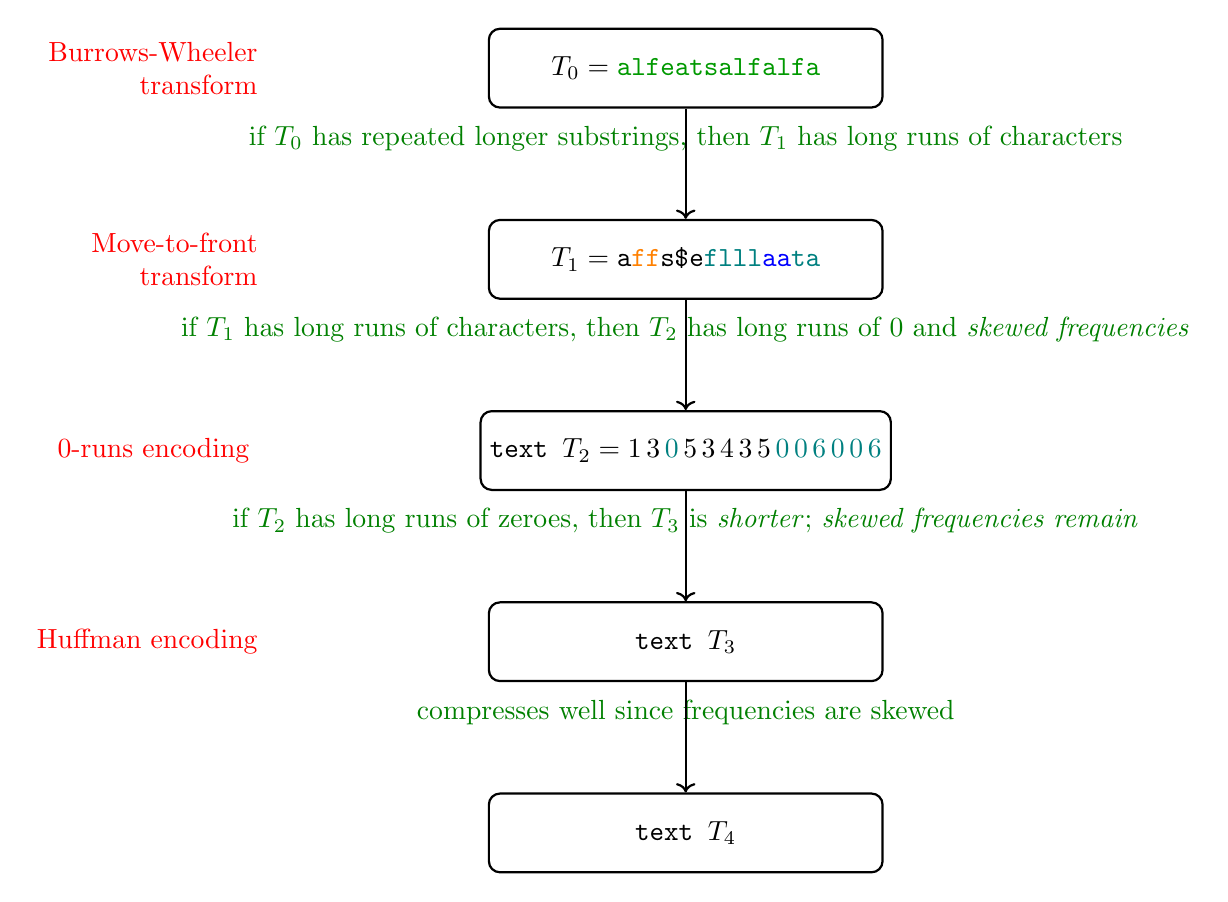
\begin{tikzpicture}[node distance=1.6cm, font=\normalsize]
            % Nodes
            \node (T0) [draw, thick, rounded corners, minimum width=5cm, minimum height=1cm] {$T_0 = \textcolor{green!60!black}{\texttt{alfeatsalfalfa}}$};
            
            \node (label1) [left=2.8cm of T0, align=right, text=red] {Burrows-Wheeler\\ transform};
            \node (note1) [below=0.1cm of T0, align=center, text=green!50!black] {if $T_0$ has repeated longer substrings,\ then $T_1$ has long runs of characters};
            
            \node (T1) [below=1.4cm of T0, draw, thick, rounded corners, minimum width=5cm, minimum height=1cm] 
            {$T_1 = \texttt{a\textcolor{orange}{ff}s\$e\textcolor{teal}{flll\textcolor{blue}{aa}ta}}$};
            
            \node (label2) [left=2.8cm of T1, align=right, text=red] {Move-to-front\\ transform};
            \node (note2) [below=0.1cm of T1, align=center, text=green!50!black] {if $T_1$ has long runs of characters,\ then $T_2$ has long runs of 0 and \textit{skewed frequencies}};
            
            \node (T2) [below=1.4cm of T1, draw, thick, rounded corners, minimum width=5cm, minimum height=1cm] 
            {\texttt{text }$T_2 = 1\,3\,\textcolor{teal}{0}\,5\,3\,4\,3\,5\,\textcolor{teal}{0\,0\,6\,0\,0\,6}$};
            
            \node (label3) [left=2.8cm of T2, align=right, text=red] {0-runs encoding};
            \node (note3) [below=0.1cm of T2, align=center, text=green!50!black] {if $T_2$ has long runs of zeroes,\ then $T_3$ is \textit{shorter}; \textit{skewed frequencies remain}};
            
            \node (T3) [below=1.4cm of T2, draw, thick, rounded corners, minimum width=5cm, minimum height=1cm] 
            {\texttt{text }$T_3$};
            
            \node (label4) [left=2.8cm of T3, align=right, text=red] {Huffman encoding};
            \node (note4) [below=0.1cm of T3, align=center, text=green!50!black] {compresses well since frequencies are skewed};
            
            \node (T4) [below=1.4cm of T3, draw, thick, rounded corners, minimum width=5cm, minimum height=1cm] 
            {\texttt{text }$T_4$};
        
            % Arrows
            \draw[->, thick] (T0) -- (T1);
            \draw[->, thick] (T1) -- (T2);
            \draw[->, thick] (T2) -- (T3);
            \draw[->, thick] (T3) -- (T4);
        \end{tikzpicture}
    \end{center}
\end{examplee}

\begin{deff}[Text Transform \index{Text Transform}].
    \textbf{Text transform} refers to changing input text into a different text. \begin{comm}[].
        Ouput is not shorter, but likely to compresses better. 
    \end{comm}
\end{deff}

\subsubsection{Move-to-Front transform} 

\begin{algo}[].
    Source alphabet is $\Sigma_S$ with size $|\Sigma_S = m|$, we first put alphabet in array $L$, initially in sorted order, but allow $L$ to get unsorted in the process: \hl{After each encoding, update $L$ with Move-To-Front heuristic}. 
\end{algo}

\begin{discovery}[].
    Dictionary $D$ is changed dynamically just like LZW, but unlike LZW, no new items added to dictionary and codeword for one or more letters can change at each iteration. 
\end{discovery}

\subsubsection{Move-to-Front Transform: Properties} 

\begin{enumerate}
    \item If a character in $S$ repeats $k$ times, then $C$ has a run of $k - 1$ zeros; 
    \item $C$ contains a lot  of small numbers and a few big ones (skewed frequencies);  
    \item $C$ has the same length as $S$, but better properties for encoding.
\end{enumerate}

\subsubsection{0-runs Encoding} 

Input consists of `characters' in $\{ 0, \ldots, 127 \}$ with long runs of zeros. We replace $k$ consecutive zeros by $(k)_2$ (takes approximately $\log k $bits) bits using two new characters $A$, $B$. 

\begin{examplee}[].
    $65, 0, 0, 0, 0, 67, 0, 0, 72$ becomes $65, A B, 67, B 72$. 
\end{examplee}

\subsection{Burrows-Wheeler Transform} 

\begin{deff}[Burrows-Wheeler Transform \index{Burrows-Wheeler Transform}].
    \textbf{Burrows-Wheeler Transform} is a transformation algorithm, it is not a compression algorithm. It transforms source text to coded text with same letters butin different order. 
\end{deff}

\begin{thmm}[].
    It is required that the source text $S$ ends with end-of-word character \$, \$ occurs nowhere else in $S$ and us counted towards length of $S$. 
\end{thmm}

\begin{comm}[].
    Burrows-Wheeler Transform is based on cyclic shifts for a string. 
\end{comm}

\begin{deff}[Cyclic Shift \index{Cyclic Shift}].
    A \textbf{cyclic shift} of string $X$ of length $n$ is the concatenation of $X[i+1, \ldots, n-1]$ and $X[0, \ldots, i]$, for $0 \leq i < n$. 
\end{deff}

\subsubsection{BWT Algorithm andExample} 

\begin{minipage}{0.5\textwidth}
    Consider 
    \[ S = \texttt{ alfeatsalfalfa\$ } \] 
    \begin{enumerate}
        \item We first write all consecutive cyclic shifts, forming an array of shifts (see the middle column). 
        \item We then sort (lexographically) cyclic shifts (see the rightmost column), note that we have strict sorting order due to \texttt{\$}. 
    \end{enumerate}
    \begin{result}[].
        Last column can be decoded. 
    \end{result}
    Hence in our example, 
    \[ C = \texttt{ affs\$eflllaaata } \]
\end{minipage} \begin{minipage}{0.25\textwidth}
    \begin{verbatim}
    alfeatsalfalfa$
    lfeatsalfalfa$a
    featsalfalfa$al
    eatsalfalfa$alf
    atsalfalfa$alfe
    tsalfalfa$alfea
    salfalfa$alfeat
    alfalfa$alfeats
    lfalfa$alfeatsa
    falfa$alfeatsal
    alfa$alfeatsalf
    lfa$alfeatsalfa
    fa$alfeatsalfal
    a$alfeatsalfalf
    $alfeatsalfalfa
    \end{verbatim}
\end{minipage} \begin{minipage}{0.3\textwidth}
    \begin{verbatim}
    $alfeatsalfalfa a
    a$alfeatsalfalf f
    alfa$alfeatsalf f
    alfalfa$alfeats s
    alfeatsalfalfa$ $
    atsalfalfa$alfe e
    eatsalfalfa$alf f
    fa$alfeatsalfal l
    falfa$alfeatsal l
    featsalfalfa$al l
    lfa$alfeatsalfa a
    lfalfa$alfeatsa a
    lfeatsalfalfa$a a
    salfalfa$alfeat t
    tsalfalfa$alfea a
    \end{verbatim}
\end{minipage}

\subsubsection{BWT Fast Encoding: Efficient Sorting}

\begin{thmm}[].
    We can read BWT encoding from suffix array in $O(n)$ time: 
    \[ C[i] = S[ A^s[i] - 1 ] \]
\end{thmm}

\begin{proof}
    $A^s[i]$ gives the starting index of the $i^{th}$ lex smallest suffix, hence taking the one before it yields us the character at the end of the row. 
\end{proof}

\subsubsection{BWT Decoding} 

\begin{discovery}[].
    In unsorted shifts array, first column is $S$, so decoding is equivalent to determining the first letter of each row in unsorted shifts array. 
\end{discovery}

\paragraph{Observation 1:} First column has exactly the same characters as the last column, and they must be sorted. Therefore, after sorting the the characters and align them with $C$, the character matches with \$ is the start of row 0. 

\paragraph{Observation 2:} if row $i$ starts with character $c$, then row $i+1$ has to end with character $c$. Moreover, if row $i$ is the $k^{th}$ among the rows start with character $c$, then row $i+1$ is the $k^{th}$ among the rows end with character $c$. 

\begin{codes}[].
    \begin{lstlisting}[style=cppstyle, mathescape=false]
    BWT::decoding(C, S)
    // C: string of characters over alphabet (*@$\Sigma_C$@*), one of which is $
    // S: output stream
    initialize array A            // leftmost column
    for all indices i of C
        A[i] (*@$\leftarrow$@*) (C[i], i)          // store character and index
    stably sort A by character (the first aspect)
    for all indices j of C        // find $
        if C[j] = $ break
    do
        S.append(character stored in A[j])
        j (*@$\leftarrow$@*) index stored in A[j]
    while appended character is not $
    \end{lstlisting}
\end{codes}

\subsubsection{BWT Summary}

\begin{discovery}[].
    BWT needs all of the text (no streaming possible). 
\end{discovery} 

\begin{result}[BWT Summary].
    \begin{enumerate}
        \item Encoding cost $O(n \log n)$ with special sorting algorithm -- read encoding from the suffix array; 
        \item Decoding cost $O(n + |\Sigma_S|)$, which is faster than encoding. 
    \end{enumerate}
    \begin{comm}[].
        Encoding and decoding both use $O(n)$ space. 
    \end{comm}
\end{result}

\subsubsection{bzip2 Summary} 

\begin{result}[].
    \begin{enumerate}
        \item encoding cost: $O (n [\log n + |\Sigma|])$ with a big multiplicative constant; 
        \item decoding cost: $O (n |\Sigma|)$ with a big multiplicative constant. 
    \end{enumerate}
\end{result}

\newpage

\subsection{Compression Summary} 

\begin{center}
    \begin{tabular}{l l l}
    \toprule
        Huffman & Lempel-Ziv-Welch & bzip2 (uses Burrows-Wheeler) \\
    \midrule
        variable-length & fixed-width & multi-step \\
        single-character & multi-character & multi-step \\
        2-pass, must send dictionary & 1-pass & not streamable \\
        optimal 01-prefix-code & good on English text & better on English text \\
        requires uneven frequencies & requires repeated substrings & requires repeated substrings \\
        rarely used directly & frequently used & used but slow \\
        part of pkzip, JPEG, MP3 & GIF, some variants of PDF, compress & bzip2 and variants \\
    \bottomrule
    \end{tabular}
\end{center}

\newpage

\section{External Memory} 

Our current architecture is: \begin{multicols}{2}
    \begin{enumerate}
        \item registers: super fast, very small  
        \item cache L1, L2: very fast, less small  
        \item main memory: fast, large  
        \item disk or cloud: slow,  very large
    \end{enumerate}
\end{multicols} 

\begin{Question}{}
    How to adapt algorithms to take memory hierarchy into consideration? 
    \begin{comm}[].
        desirable to minimize transfer between slow/ fast memory. 
    \end{comm}
\end{Question}

\subsection{Stream based algorithms} 

We studied algorithms that handle input/ output with streams, recall: 
\begin{enumerate}
    \item take item off top of the input; 
    \item process item output; 
    \item put the result of processing at the tail of output. 
\end{enumerate}

\begin{discovery}[].
    Data in external memory has to be  placed in internal memory before it can be processed. 
\end{discovery}

\begin{solution}
    perform the same algorithm as before, but in ``block-wise'' manner: 
    \begin{itemize}
        \item have one block for input, one block for output in internal memory 
        \item transfer a block (size $B$) to internal memory, process it as before, store result in output block 
        \item when output stream is of size $B$ (full block), transfer it to external memory 
        \item when current block is in internal memory is fully processed, transfer next unprocessed block from external memory
    \end{itemize}
\end{solution}

\begin{result}[].
    Methods below use stream input/output model, therefore need $\Theta \left( \dfrac{n}{B} \right)$ transfers, if output size is $O(n)$. 
    \begin{enumerate}
        \item Pattern matching: Karp-Rabin, Knuth-Morris-Pratt, Boyer-Moore
        \begin{comm}[].
            assuming pattern $P$ fits into internal memory 
        \end{comm}
        \item Text compression: Huffman, run-length encoding, Lempel-Ziv-Welch
        \item Sorting: merge-sort can be implemented with $O \left( \dfrac{n}{B} \log n \right)$ block transfers 
        \item Bzip2 cannot be streamed as we described
        \begin{comm}[].
            can compress in `blocks', though not as good as the whole text compression, but better than nothing. 
        \end{comm}
    \end{enumerate}
\end{result}

\subsection{External dictionaries}

AVL tree based dictionary implementations have poor \textit{memory locality}, meaning `nearby' tree nodes are unlikely to be in the same block.

\begin{discovery}[].
    In an AVL tree $\Theta(\log n)$ blocks are loaded in the worst case. 
\end{discovery}

\begin{proof}
    Each AVL tree node could be stored in a different disk block, so you might have to load up to $O(\log n)$ different blocks just to follow one path.
\end{proof}

\begin{thmm}[].
    Idea: allow trees that have many children per node. 
\end{thmm}

\begin{examplee}[].
    suppose store $n = 2^{50}$ items total, and $B = 2^{15}$ children per node, tree height is 
    \[ \log_B n = \frac{\log_2 n}{\log_2 B} = \frac{50}{15} \]
    which means that it is 15 times less block transfers. 
\end{examplee}

\subsection{2-4 Trees} 

\begin{deff}[2-4 Tree \index{2-4 Tree}].
    \begin{enumerate}
        \item \texttt{Structural properties}: Every node is either 
        \begin{itemize}
            \item 1-node: one KVP and two subtrees (possibly empty), or 
            \item 2-node: two KVPs and three subtrees (possibly empty), or 
            \item 3-node: three KVPs and four subtrees (possibly empty)
            \begin{comm}[].
                Allowing 3 types of nodes simplifies insertion/ deletion. 
            \end{comm}
            \item All empty subtrees are at the same level. (necessary for ensuring height is logarithmic in the number of KVP stored).  
        \end{itemize}
        \item \texttt{Order Property}: keys at anynode are between the keys in the subtrees. 
    \end{enumerate}
\end{deff}

\begin{thmm}[].
    The height of a 2-4 tree is $O(\log n)$. 
\end{thmm}

\begin{proof}
    Proof is given in the section (a,b)-tree, since 2-4 tree is a special case of (a,b)-tree. 
\end{proof}

\begin{comm}[].
    \hl{Empty subtrees are not part of height computation} (Often times, we do not even show empty subtrees). 
\end{comm}

\subsubsection{2-4 Tree, Search}

\begin{codes}[].
    \code{search($k$)} compares key $k$ to $k_1$, $k_2$, $k_3$, and either finds $k$ among $k_1$, $k_2$, $k_3$ or figures out which subtree to recurse into. If key is not in tree, search returns parent of empty tree where search stops. 
\end{codes}

\begin{codes}[].
    \begin{lstlisting}[style=cppstyle]
        24Tree::search($k$, $v \leftarrow$ root, $p \leftarrow$ empty subtree)
        $k$: key to search, $v$: node where we search; $p$: parent of $v$
        
        if $v$ represents empty subtree
            return "not found, would be in $p$"
        let $\langle T_0, k_1, \ldots, k_d, T_d \rangle$ be key-subtrees list at $v$
        if $k \geq k_1$
            $i \leftarrow$ maximal index such that $k_i \leq k$
            if $k_i = k$
                return "at $i$th key in $v$"
            else `24Tree::search`($k$, $T_i$, $v$)
        else `24Tree::search`($k$, $T_0$, $v$)
    \end{lstlisting}
\end{codes}

\subsubsection{2-4 Tree, Insert}

\begin{codes}[].
    \begin{lstlisting}[style=cppstyle]
    24Tree::insert($k$)
        $v \leftarrow$ 24Tree::search($k$) // leaf where $k$ should be
        add $k$ and an empty subtree in key-subtree-list of $v$

        while $v$ has 4 keys (overflow $\rightarrow$ node split!)
            let $\langle T_0, k_1, \ldots, k_4, T_4 \rangle$ be key-subtrees list at $v$
            if $v$ has no parent
                create an empty parent of $v$
            $p \leftarrow$ parent of $v$
            $v' \leftarrow$ new node with keys $k_1, k_2$ and subtrees $T_0, T_1, T_2$
            $v'' \leftarrow$ new node with key $k_4$ and subtrees $T_3, T_4$
            replace $\langle v \rangle$ by $\langle v', k_3, v'' \rangle$ in key-subtree-list of $p$
            $v \leftarrow p$ @// continue checking for overflow upwards@
    \end{lstlisting}
\end{codes}

\begin{examplee}[].
    Here is an example of node splitting: \begin{center}
        \includegraphics[width=0.8\textwidth]{img/nodesplitting.png}
    \end{center}
\end{examplee}

\begin{deff}[Immediate Sibling \index{Immediate Sibling}].
    A node can have an immediate left sibling, immediate right sibling, or both. 
    \begin{comm}[].
        Any node except the root must have an immediate sibling. 
    \end{comm}
\end{deff}

\begin{deff}[In Order Successor \index{In Order Successor}].
    \textbf{Inorder successor} of key $k$ is the smallest key in the subtree immediately to the right of $k$. 
\end{deff}

\begin{discovery}[].
    Inorder successor is guaranteed to be at a leaf node. 
\end{discovery}

\begin{proof}
    Otherwise would have something smaller in the leftmost subtree. 
\end{proof}

\subsubsection{2-4 Tree, Delete} 

\begin{result}[].
    \begin{enumerate}
        \item If key not at a leaf node, swap with inorder successor (guaranteed at leaf node) 
        \item Delete key and one empty subtree from the leaf node involved in swap 
        \item If underflow \begin{itemize}
            \item If there is an immediate sibling with more than one key, transfer \begin{itemize}
                \item no further underflows caused, do not forget to transfer a subtree as well 
                \item convention: if two siblings have more than one key, transfer with the right sibling
            \end{itemize}
            \item If all immediate siblings have only one key, merge 
            \begin{itemize}
                \item there must be at least one sibling, unless root, if root, delete 
                \item convention: if two immediate siblings with one key, merge with the right one 
                \item merge may cause underflow at the parent node, continue to the parent and fix it, if necessary
            \end{itemize}
        \end{itemize}
    \end{enumerate}
\end{result}

\begin{codes}[].
    \begin{lstlisting}[style=cppstyle]
    24Tree::delete($k$)
        $v \leftarrow$ 24Tree::search($k$) // node containing $k$
        if $v$ is not a leaf
            swap $k$ with its inorder successor $k'$
            swap $v$ with leaf that contained $k'$
        delete $k$ and one empty subtree in key-subtree-list of $v$
        while $v$ has 0 keys // underflow
            if $v$ is the root, delete $v$ and break
            if $v$ has immediate sibling $u$ with 2 or more KVPs // transfer, then done!
                transfer the key of $u$ that is nearest to $v$ to $p$
                transfer the key of $p$ between $u$ and $v$ to $v$
                transfer the subtree of $u$ that is nearest to $v$ to $v$
                break
            else // merge and repeat
                $u \leftarrow$ immediate sibling of $v$
                transfer the key of $p$ between $u$ and $v$ to $u$
                transfer the subtree of $v$ to $u$
                delete node $v$
                $v \leftarrow p$
    \end{lstlisting}
\end{codes}

\subsection{Red Black Tree} 

\begin{discovery}[].
    Problem with 2-4 trees: 
    \begin{Question}{}
        How should we store keys and subtrees? 
    \end{Question}
    \begin{comm}[].
        array of length 7 wastes space; linked list overhead for list-nodes, also wastes space. Theoretical bound not affected, but matters in practice. 
    \end{comm}
\end{discovery}

\begin{solution}
    Design a class of binary search trees that mirrors 2-4 tree. 
\end{solution}

\subsubsection{2-4 Tree to Red Black Tree} 

There are three types of nodes in 2-4 tree: 
\[ \texttt{1-node}, \quad \texttt{2-node}, \quad \text{and } \texttt{3-node} \]

\begin{algo}[].
    $d$-node becomes a black node with $d-1$ red children (assembled in a way so that they form a BST of height at most 1). 
\end{algo}

\begin{deff}[Overhead \index{Overhead}].
    Red/ black `colour' is stored with just 1 extra bit per node. 
\end{deff}

\begin{result}[].
    \begin{itemize}
        \item Any red node has a black parent; 
        \item Any empty subtree of $T$ has the same black-depth.
        \begin{deff}[Black-depth \index{Black-depth}].
            \textbf{Black-depth} refers to the number of black nodes on the path from root to $T$. 
        \end{deff}
    \end{itemize}
\end{result}

\begin{examplee}[].
    Here is an example converting 2-4 tree to red black tree: 
    \begin{center}
        \includegraphics[width=0.7\textwidth]{img/24toredblack.png}
    \end{center}
\end{examplee}

\subsubsection{Red Black Tree to 2-4 Tree} 

\begin{thmm}[]. 
    Any red-black tree can be converted to a 2-4 tree. 
\end{thmm}

\begin{proof}
    black node with $0 \leq d \leq 2$ red children becomes a $(d + 1)$-node, and this covers all nodes, as no red node has a red child. Empty subtrees on the same level due to the same blackdepth. 
\end{proof}

\begin{examplee}[].
    Here is an example converting red black tree to a 2-4 tree: 
    \begin{center}
        \includegraphics[width=0.7\textwidth]{img/redblackto24.png}
    \end{center}
\end{examplee}

\subsubsection{Red Black Trees Summary} 

\begin{result}[].
    \begin{itemize}
        \item Red-black trees have height $O(\log n)$, each level of 2-4 tree creates at most 2 levels in red-black tree. 
        \item Insert/delete can be done in $O(\log n)$ time \begin{itemize}
            \item convert relevant part to 2-4 tree 
            \item do insert/delete as in 2-4 tree 
            \item convert relevant parts back to red-black tree
        \end{itemize}
        \item Insert/delete can be done in $O(\log n)$ without conversion. 
    \end{itemize} 
\end{result}

\begin{comm}[].
    Red/ black trees are very popular balanced search trees (\code{std::map}).
\end{comm}

\newpage

\subsection{(a,b)-tree} 

\begin{deff}[(a,b)-tree \index{(a,b)-tree}].
    $(a,b)$-tree satisfies \begin{enumerate}
        \item each node has at least $a$ subtrees, unless it is the root (root must have at least 2 subtrees); 
        \item each node has at most $b$ subtrees; 
        \item if node has $d$ subtrees, then it stores $d-1$ key-value pairs (KVPs); 
        \item all empty subtrees are at the same level; 
        \item keys in the node are between keys in the corresponding  subtrees; 
        \item requirement: $b \geq 3$ and $2 \leq a \leq \lceil b/2 \rceil$. 
        \begin{comm}[].
            Lower bound on $a$ is needed to bound height, upper bound on $a$ is needed during operations. 
        \end{comm}
    \end{enumerate}
\end{deff}

\begin{Question}{}
    Why special condition for the root? 
\end{Question}

\begin{solution}
    Otherwise we could not build the tree if for example, we force the root to have at least three children but we only have one KVP. 
\end{solution}

\begin{thmm}[].
    Height of (a,b)-tree with $n$ KVPs is $O(\log_a n)$. 
\end{thmm}

\begin{proof}
    Consider (a,b)-tree with the smallest number of KVP and of height $h$ (red node (the root)  has 1 KVP, blue nodes have $(a-1)$ KVP). 
    \begin{center}
        \includegraphics[width=0.8\textwidth]{img/abtreeheight.png}
    \end{center}
    Hence we have 
    \[ \# \text{ of KVPs} = 1 + \sum_{i=0}^{h-1} 2a^i(a - 1)
    = 1 + 2(a - 1) \sum_{i=0}^{h-1} a^i 
    = 2a^h - 1 \]
    Let $n$ the number of KVP in any (a,b)-tree of height $h$, then 
    \[ n \geq 2 a^h - 1 \qquad \rightarrow \qquad \log_a \frac{n + 1}{2} \geq h \]
    which implies that the height of a tree with $n$ KVPs is $O(\log_a n) = O(\log n / \log a)$.
\end{proof}

\begin{thmm}[].
    number of of KVP $=$ number of empty subtrees $- 1$ in any (a,b)-tree. 
\end{thmm}

\begin{proof}
    Put one stone on each empty subtree and pass the stones up the tree. Each node keeps 1 stone per KVP, and passes the rest to its parent. Since for each node, \#KVP $=$ \# children $- 1$, each node will pass only 1 stone to its parent.  This process stops at the root, and the root will pass 1 stone outside the tree. At the end, each KVP has 1 stone, and 1 stone is outside the tree. 
\end{proof}

\subsection{B-tree} 

\begin{comm}[].
    B-tree is a type of (a,b)-tree tailored to the external memory model. Each block in external memory stores one tree node. 
\end{comm}

\begin{deff}[B-tree \index{B-tree}].
    \textbf{B-tree} is (a,b)-tree such that $a = \lceil a / 2 \rceil$. 
\end{deff}

\begin{comm}[].
    For external memory, choose $b$ s.t. the largest possible node (i.e. $b$ subtrees) fits into a block. 
\end{comm}

\newpage

\section{Post-Midterm/ Final} 

\begin{exer}[]. 
    \begin{cate}[Hashing (with Linear Probing)]. \end{cate}
    Suppose we have a hash table of size 7 and we use Linear Probing with the following hash function: 
    \[ h(k, i) = ((k \bmod 6) + i) \bmod 6 \]
    Assuming each hash value is equally likely for a given key, what is the probability that slots 2, 3, and 4 are occupied after we insert 3 elements into the hash table?
\end{exer}

\begin{solution}
    Poossible orders of hashing that result in slots 2, 3, and 4 being occupied are: \begin{center}
        \begin{tabular}{|c c c|} \hline
            \texttt{2 3 4} & \texttt{2 2 4} & \texttt{3 3 2} \\ 
            \texttt{2 4 4} & \texttt{2 2 3} & \texttt{3 2 2} \\ 
            \texttt{3 2 4} & \texttt{2 2 2} & \texttt{3 2 3} \\ 
            \texttt{3 4 2} & \texttt{2 3 3} & \texttt{4 2 2} \\ 
            \texttt{4 3 2} & \texttt{2 3 2} & \\ 
            \texttt{4 2 3} & \texttt{2 4 2} & \\ \hline
        \end{tabular}
    \end{center} 
    In total 16 possibilities, thus the probability is $\dfrac{16}{6^3}$. 
\end{solution}

\begin{exer}[].
    \begin{cate}[Cuckoo Hashing]. \end{cate}
    T/ F: In cuckoo hashing, search and delete have guaranteed $O(1)$ run-time.
\end{exer}

\begin{solution}
    True. 
\end{solution}

\begin{exer}[]. 
    \begin{cate}[Hashing, Hashing Function Property]. \end{cate}
    What is the desired property of a randomly chosen hash function $h : U \rightarrow \{ 0, 1, \ldots, S-1 \}$? \begin{enumerate}
        \item It is a one-to-one function. 
        \item $S \geq U$ 
        \item $\Pr(h(u) = i) = \frac{1}{S} \quad \text{for all keys } u \text{ and slots } i$
        \item $\text{For } u, v \in U, \; h(u) \ne h(v)$
    \end{enumerate}
\end{exer}

\begin{solution}
    3 is the right answer. 
\end{solution}

\begin{exer}[].
    The height $h$ of a 2-dimensional $kd$-tree is never larger than the height of a 2-dimensional quadtree where both trees store the same $n$ 2-dimensional points in general position (i.e.\ distinct $x$ and $y$ coordinates) and $h > 0$.
\end{exer}





















\printindex

\end{document}